\documentclass[a4paper, 12pt, openright, oneside, german, french, english, brazil]{abntex2}
\usepackage[brazil]{babel}
\usepackage{graphicx}
\usepackage[utf8]{inputenc}
\usepackage{wrapfig}
\usepackage{lscape}
\usepackage{rotating}
\usepackage{epstopdf}
\usepackage[alf]{abntex2cite}
\usepackage[a4paper, left=3cm, right=2cm, top=3cm, bottom=2cm]{geometry}
\usepackage{indentfirst}
\usepackage{longtable}
\usepackage{amsmath}
\usepackage{verbatim}
\usepackage{algorithm}
\floatname{algorithm}{Código}
\renewcommand{\listalgorithmname}{Lista de Códigos}
\usepackage{algpseudocode} %para escrever pseudo-algoritmos
%\algrenewcommand\algorithmicwhile{\textbf{Enquanto}}
%\algrenewcommand\algorithmicfor{\textbf{Para}}
%\algrenewcommand\algorithmicif{\textbf{Se}}
%\algrenewcommand\algorithmicthen{\textbf{então}}
%\algrenewcommand\algorithmicelse{\textbf{Do contrário}}
%\algrenewcommand\algorithmicdo{\textbf{faça}}
%\algrenewcommand\algorithmicfunction{\textbf{Função}}
%\algrenewcommand\algorithmicend{\textbf{termina}}
\usepackage{listings} %para escrever códigos
\pagestyle{plain}

\titulo{\textbf{A Construção Social de Prestígio e Valor no Mercado da Música de Concerto}}
\autor{Neylson J. B. F. Crepalde}
\data{Fevereiro, 2019}
\instituicao{UNIVERSIDADE FEDERAL DE MINAS GERAIS
	\par
	Faculdade de Filososia e Ciências Humanas}
\local{Belo Horizonte}
\orientador{Dr. Silvio Salej Higgins}
\preambulo{Tese apresentada ao programa de pós-graduação em sociologia como requisito parcial à obtenção do título de Doutor em Sociologia. Linha de Pesquisa: Sociologia Econômica e das Organizações}
\tipotrabalho{Tese (doutorado)}


\begin{document}
	\pretextual
	%\imprimircapa
	\imprimirfolhaderosto
	
	%	\begin{dedicatoria}
	%		\vspace*{\fill}
	%		Dedico este trabalho a \ldots
	%		\vspace*{\fill}
	%	\end{dedicatoria}
	
	%\begin{agradecimentos}
	%	Gostaria de agradecer \ldots
	%\end{agradecimentos}
	
	%\begin{epigrafe}
	%	\vspace*{\fill}
	%	\begin{flushright}
	%		\textit{Não é da benevolência do violinista, do maestro e do diretor artístico que esperamos a nossa \textbf{música}, mas da consideração que ele tem pelos prórprios interesses.\\
	%			(parafraseando Adam Smith)}
	%	\end{flushright}
	%\end{epigrafe}
	
	%% --- resumo em português ---
	%\begin{resumo}
	%	Resumo em português\\
	%	\vspace{\onelineskip}
	%	\noindent
	%	\textbf{Palavras-chave}: latex. abntex. editoração de texto.
	%\end{resumo}
	%% --- resumo em inglês ---
	%\begin{resumo}[Abstract]
	%	\begin{otherlanguage*}{english}
	%		The abstract in english.\\
	%		\vspace{\onelineskip}
	%		\noindent
	%		\textbf{Keywords}: latex. abntex. publication of texts.
	%	\end{otherlanguage*}
	%\end{resumo}
	%% --- resumo em francês ---
	%\begin{resumo}[Résumé]
	%	\begin{otherlanguage*}{french}
	%		Il s’agit d’un résumé en français.\\
	%		\vspace{\onelineskip}
	%		\noindent
	%		\textbf{Mots-clés}: latex. abntex. publication de textes.
	%	\end{otherlanguage*}
	%\end{resumo}
	
%	\listofalgorithms
	\listoffigures
	\listoftables	
	\newpage
	\tableofcontents
	\textual
	
	\chapter*[Introdução]{Introdução}
	\addcontentsline{toc}{chapter}{INTRODUÇÃO}
	
	Para que o produto final por excelência de uma orquestra, a saber os concertos, venha a existir e chegue ao seu destino, o público, uma série de atores se envolvem em diversos processos de cooperação e mobilizam uma série de recursos construindo um sistema de produção em rede, ou o que Howard Becker chamaria de um ``mundo da arte'' (\textit{Art World}). Para \citeonline[p. 1, tradução do autor]{becker2008art}, ``a existência de mundos da arte, bem como o modo como sua existência afeta tanto a produção quanto o consumo de obras de arte, sugere uma abordagem sociológica para as artes'' \footnote{The existence of art worlds, as well as the way their existence affects both the production and consumption of art works, suggests a sociological approach to the arts.}.
	
	\begin{citacao}
		Os mundos da arte consistem de todas as pessoas cujas atividades são necessárias para a produção de obras características que aquele mundo, e talvez outros ainda, definem como arte. Membros dos mundos da arte coordenam as atividades pelas quais a obra é produzida referindo-se a um corpo de entendimentos convencionais incorporados na prática comum e nos artefatos comumente usados. As mesmas pessoas frequentemente cooperam repetidamente, até mesmo rotineiramente, de formas similares para produzir obras similares, portanto podemos pensar em um mundo da arte como uma rede de conexões de cooperação entre os participantes estabelecida.\footnote{Art worlds consist of all the people whose activities are necessary to the production of the characteristic works which that world, and perhaps others as well, define as art. Members of art worlds coordinate the activities by which work is produced by referring to a body of conventional understandings embodied in common practice and in frequently used artifacts. The same people often cooperate repeatedly, in similar ways to produce similar works, so that we can think of an art world as an established network of cooperative links among participants.} \cite[p. 34-5]{becker2008art}
	\end{citacao}
	
	Para que os concertos aconteçam, a orquestra (formada pelos instrumentistas, pelo maestro, pela administração e ainda pela instituição mantenedora) toca uma obra escrita por um compositor em uma notação convencionada. Os instrumentistas tocam em instrumentos construídos por um luthier de uma maneira também convencionada. Para que o concerto aconteça, é preciso que exista uma demanda por ele. Por isso, além da orquestra, participam do evento o público consumidor do espetáculo, os meios de divulgação pelos quais esse público toma conhecimento do concerto, o Estado como regulador e financiador, as empresas privadas que também financiam a orquestra, além de diversos outros atores com papeis menores, embora igualmente importantes (iluminadores, técnicos de som, funcionários da bilheteria, copistas, arquivistas, montadores, etc.).
	
	O mesmo fenômeno é abordado por \citeonline{lazega2009theorie} mas de uma perspectiva distinta: no mundo concorrencial, os atores se veem constantemente em situações em que buscam a estabilidade do mercado tornando-o viável. Isso não acontece simplesmente de acordo com a lei da oferta e da demanda mas a partir do posicionamento dos produtores numa escala de qualidade que diferencia seus produtos. Para que isso seja possível, a concorrência total é inviável já que existe uma parcela de interdependência entre produtores. Para o autor, ``a construção coletiva da qualidade implica que a viabilidade do mercade vem do coletivo, e que é a estrutura do conjunto do mercado viável que cria a divisão de lucros\footnote{La construction collective de la qualité implique ainsi que la viabilité du marché vient du collectif, et que c'est la structure d'ensemble du marché viable qui crée le partage des rentes.}'' \cite[p. 563, tradução do autor]{lazega2009theorie}. 
	
	Desse modo, para que esse mercado viável seja possível, é necessário que que as empresas se engajem constantemente numa combinação estável de concorrência e de cooperação. A emergência de uma estrutura a partir das próprias relações assimétricas entre eles pode criar vantagens para alguns. Para \citeonline{lazega2009theorie}, ``as relações de poder e os controles que eles exercem sobre as negociações são, portanto, cruciais nesse modelo. Sobre esse tipo de mercado, por definição, a troca não é jamais bilaterial, sempre multilateral e estratégica\footnote{Les relations de pouvoir et les contraintes qu'elles font peser sur les négociations sont donc cruciales dans ce modèle. Sur ce type de marché, par définition, l'échange n'est jamais bilatéral, toujours multilatéral et stratégique.}'' \cite[p. 563, tradução do autor]{lazega2009theorie}. Esse fenômeno é conhecido na literatura como \textit{coopetition}. A partir das perspectivas apresentadas, entramos na problemática que conduz nossa investigação.
	
	
	
	\subsection*{Problemas de Pesquisa}
	%\addcontentsline{toc}{section}{Problema de Pesquisa e Objetivos}
	
	Este trabalho visa debruçar-se sobre o mercado da música de concerto na região Sudeste do Brasil. A investigação é norteada por duas principais perguntas: 1) Entendendo que o mercado das orquestras não opera como um mercado comum, como se dá seu funcionamento; quem são os atores envolvidos e quais são as ações que cada um desenvolve no sistema? 2)Quais são as condições e fatores sociais de produção de padrões de qualidade da música de concerto, ou seja, como é produzido e mantido o \textit{standard} de qualidade com o qual todos estão comprometidos?
	
	Para desenvolvermos nosso estudo faz-se necessário transcender os limites com os quais a teoria econômica se deparou ao abordar produtos culturais. Ora, em todo o seu decurso, a teoria econômica tem ancorado seus principais achados em dois pressupostos. O primeiro remonta à ideia do \textit{homo economicus}, ou seja, o ator racional que toma decisões visando potencializar ganhos e diminuir perdas. Para isso, ele tem acesso à completude das informações de que precisa e é capaz de processá-las inteiramente. Esse pressuposto dá à economia a capacidade de elaborar modelos elegantes para explicar escolhas e preferências mas não consegue incorporar uma parte central da vida social, a saber, a cultura. A área da sociologia econômica desenvolveu-se, sobretudo, se debruçando sobre as lacunas deixadas por esse pressuposto buscando dar conta de como normas sociais, valores, sistemas de status e prestígio influenciam a ação econômica. Dito de outra forma, uma perspectiva sociológica possibilita enxergar fatores relacionais que ajudam a responder a perguntas clássicas da economia além de tornar o estudo mais próximo da realidade mesmo não tendo modelos tão elegantes e nem lógica tão consistente \cite{hirsch1987dirty}. A sociologia econômica está preocupada com elementos contextuais das trocas econômicas, ou seja, analisar como as interações entre os atores fazem emergir um mercado e como essas interações regulam e controlam os mercados.
	
	
	
	
	
	O segundo pressuposto consiste da caracterização geral dos produtos mercantis. Nessa caracterização, as mercadorias são entendidas por meio de quatro critérios objetivos, a saber, suas propriedades físicas (as quais, nesse caso, estão diretamente relacionadas com a qualidade do produto em questão), a data e o local em que estão disponíveis e aquilo que condiciona sua entrega num universo certo, i.e., sem incertezas. A qualidade de um bem, nessa perspectiva, pode ser decomposta em uma série de elementos objetivos, i.e., claramente mensuráveis e hierarquizáveis. Além disso, na teoria econômica clássica todo bem é considerado um ``bem privado'' e, portanto, ``exclusivo e rival'' no consumo. Para citar um exemplo, ``um café, um sanduíche, uma camisa, um par de sapatos, uma cadeira, etc., são bens exclusivos porque é possível impedir-me de obtê-los (\ldots); por outro lado, cada um desses bens é de consumo exclusivo porque no momento em que o aproveito, nenhuma outra pessoa pode usufruí-lo'' \cite[p. 29]{tolila2007cultura}. Ora, os produtos culturais, de um modo geral, são não exclusivos; pode-se, por exemplo, admirar um belo edifício histórico na rua sem ter que pagar por isso. Tampouco são rivais no consumo; o prazer de assistir um concerto não é diminuído pela presença de outras pessoas no público.
	
	O setor cultural define-se, ainda, pela sua lógica de oferta voltada à produção, ao contrário dos mercados de bens comuns voltados ao consumo. Para \citeonline[p. 32]{tolila2007cultura}, ``essa lógica da oferta caracteriza bem, entre outras, a ação das políticas públicas em termos de investimento, de ajuda e de sustentação das atividades culturais, do patrimônio ao espetáculo ao vivo, e em termos de incentivos às práticas culturais''. De fato, os Estados e coletividades públicas tem demonstrado interesse crescente no setor cultural, o que pode ser verificado através das políticas públicas, das administrações especializadas, da alocação de recursos dirigidos especificamente ao setor e do surgimento de toda uma rede de instituições e profissionais atuantes no setor cultural, grande parte deles financiados por dinheiro público \cite{tolila2007cultura}.
	
	O valor simbólico dos bens culturais constitui, para nós, um elemento central na compreensão de nosso objeto de estudo, muito embora, contrariando novamente a teoria econômica clássica, não seja objetivo em sua natureza mas relacional e individual, i.e., só existe à medida que é reconhecido pelo indivíduo no momento de seu consumo. Para que o valor simbólico de um determinado bem seja reconhecido, é necessário que haja estruturas cognitivas apropriadas para a compreensão e fruição do bem, ou seja, esquemas mentais adquiridos por meio da educação artística prévia \cite{bourdieu2003amor}.
	
	As performances musicais possuem ainda uma particularidade quanto à natureza de sua existência na qual reside grande parte das dificuldades metodológicas que as cercam. \citeonline{tolila2007cultura} explica:
	
	\begin{citacao}
		O que é a música? A partitura escrita? Não. Os músicos que formam a orquestra? Não. O regente? Também não. Na verdade, é quase impossível definir a música como uma ``coisa'' (uma mesa, uma cadeira, uma casa, etc.) pois ela só existe de fato no momento em que é ouvida, isto é, em uma relação com o ouvinte\footnote{Para o autor, ``na verdade, no mundo social, o modo real de existência da maioria dos fenômenos é o da relação entre seres humanos'' \cite[p. 110]{tolila2007cultura}. Curiosamente, nessa premissa se baseia todo o paradigma neoestrutural na sociologia conhecido também como ``perspectiva relacional'' ou ``teoria das redes sociais''.}. \cite[p. 109]{tolila2007cultura}
	\end{citacao}
	
	Desse modo, a música (bem como a dança e o teatro, por exemplo) assume um modo especial de existência que envolve a participação de todos os elementos ou atores supracitados, a saber, partitura, músicos, regente, etc., na construção de sua materialidade que só existe (e portanto só é possível de ser consumida) no momento da escuta.
	
	\citeonline{karpik2009elements} trata o mesmo objeto sob a ótica da ``economia de singularidades''. Para esse autor, bens e serviços singulares ``são desconhecidos pela teoria econômica neoclássica. Eles não existem''\footnote{(\dots) ils sont donc méconnus par la théorie économique néo-classique. Ils n'existent pas.} \cite[p. 163]{karpik2009elements}. As singularidades são sinalizadas pela presença do \textit{bom} em sua caracterização como diferencial numa comparação entre qualidades, i.e., o bom vinho, a boa música, a boa orquestra, etc. 
	
	\begin{citacao}
		As singularidades são bens e serviços \textit{estruturados, incertos e incomensuráveis}. Essas três características \textit{combinadas} caracterizam todas as singularidades como sendo únicas, múltiplas e seu suporte material prescinde da produção industrial, uma vez que seja mantido o seu poder simbólico e, por conseguinte, sua capacidade de acolher um número indeterminado de interpretações particulares\footnote{Les singularités sont des biens et services \textit{structurés, incertains et incommensurables.} Ces trois traits \textit{combinés} caractérisent toutes les singularités que'elles soient uniques, multiples ou que leurs supports matériels relèvent de la production industrielle, dès lors qu'est maintenu leur pouvoir symbolique et, par voie de conséquence, leur capacité à accueillir un nombre indéterminé d'interprétations particulières.}. \cite[p. 164]{karpik2009elements}
	\end{citacao}
	
	
	
	
	
	% Segundo \citeonline[p. 54]{benhamou2007economia} ``a concorrência assume a forma paradoxal de uma competição entre instituições que oferecem bens únicos e efêmeros'' onde o comportamento dos atores econômicos tende a monopólios discriminatórios. Para essa autora, o setor é caracterizado por uma fragilidade constante devido a elevações periódicas de custos e à quase-ausência de reservas de produtividade. De fato, como veremos, o paradigma vigente, no que tange a teoria econômica das performances ao vivo, aponta para um inevitável estado deficitário.
	
	
	
%	\subsection*{Justificativa}
	
	
%	Para além de seu ineditismo e originalidade, a presente proposta se justifica por duas principais razões. A primeira reside no aprendizado e desenvolvimento de habilidades e competências num dos mais atualizados paradigmas de pesquisa nas ciências humanas, a saber, a análise de redes sociais, com um de seus principais expoentes no mundo, o prof. Emmanuel Lazega. No Brasil, o número de pesquisadores trabalhando sob a ótica deste paradigma tem crescido exponencialmente. A oportunidade de ter acesso aos últimos avanços na área junto ao pesquisador que hoje ocupa a linha de frente nessa área será de grande benefício à ciência brasileira. (REVISAR)
	
%	A segunda razão reside nas possibilidades de avanços tanto na socioeconomia brasileira quanto no entendimento do funcionamento das orquestras brasileiras e de seu mercado. \ldots
	
	
	
	
	
	%\section*{Objetivos}
	
	
	\subsection*{Objetivo geral}
	
	
	\begin{itemize}
		\item Entender o funcionamento dos mercados de produção da música de concerto, sua construção, emergência, características topológicas e padrões de emergência.
	\end{itemize}
	
	\subsection*{Objetivos específicos}
	
	\begin{itemize}
		\item Mapear e analisar o mercado de produção da música de concerto nas cidades selecionadas para o estudo, a saber, Belo Horizonte, São Paulo, Hastings (Inglaterra) e Paris (França).
		\item Explicar, através de modelagem estatística de redes, a emergência da estrutura do mercado;
		\item Analisar a construção de status e prestígio entre as orquestras das capitais supracitadas;
	\end{itemize}
	
	\subsection*{Metodologia}
	
	Visando a melhor compreensão do objeto de estudo aqui proposto, a investigação será desenvolvida sob o paradigma neoestrutural ou relacional. Neste paradigma, os indivíduos não são tomados como unidade de análise conforme os estudos clássicos em sociologia, mas a unidade de análise mínima torna-se a díade.
	
	Segundo \citeonline{denooy2011exploratory}, indivíduos podem construir laços diretamente entre si por onde fluem recursos, informação, status, etc. Por outro lado, a participação deles em eventos ou sua membresia em instituições ou organizações dá origem a um laço indireto entre indivíduos e entre instituições.
	
	\begin{citacao}
		Na ciência política, economia e sociologia, muita atenção tem sido dada à composição de conselhos em grandes corporações. (\dots) Se uma pessoa é membro de um conselho de diretores em duas companhias, ele ou ela (\dots) é um diretor múltiplo que cria um diretorado conectivo ou uma conexão entre firmas. A rede de diretorados conectivos nos diz algo sobre a organização de um setor de negócios. É assumido que diretorados conectivos são canais de comunicação entre firmas\footnote{In political science, economy, and sociology, much attention has been paid to the composition of the boards of large corporations. (\dots) If a person is a member of the board of directors in two companies, he or she (\dots) is a multiple director who creates an interlocking directorate or interlock between firms. The network of interlocking directorates tells us something about the organization of a business sector. It is assumed that interlocking directorates are channels of communication between firms.}. \cite[p. 117]{denooy2011exploratory}
	\end{citacao}
	
	A perspectiva relacional parece ser a mais adequada nos dias atuais para entender fenômenos de mercado. Ela permite visualizar e modelizar estruturas sociais, o que antes não era possível. Desse modo, reconstruiremos a estrutura em rede do mercado da música de concerto nas cidades selecionadas, a saber, São Paulo, Belo Horizonte, Hastings (Inglaterra) e Paris (França). A \textbf{Análise de Redes Sociais} possui um ferramental analítico próprio que permite investigar posicionamento, prestígio, papeis sociais e até mesmo, de acordo com \citeonline{lazega2009theorie}, identificar a emergência de nichos de mercado através da modelagem de blocos (\textit{blockmodeling}).
	
%	A construção social do status das orquestras bem como os padrões de qualidade percebidos serão investigados através de modelos de difusão social em rede (\textit{network diffusion models}). Esses modelos investigam, através de simulações computacionais, o fluxo e difusão de informação e a emergência de padrões de qualidade com os quais os atores assumem compromisso \cite{valente2005network}.
	
	
	
	
	
	
	
	
	O trabalho está dividido da seguinte forma: no primeiro capítulo, faremos uma breve contextualização da formação do campo de investigação da sociologia econômica apresentando seus principais problemas e métodos e concluindo com a apresentação da literatura que proporciona a base teórica da investigação. No segundo capítulo, apresentaremos uma descrição profunda e detalhada da articulação do mercado de música erudita na região sudeste do Brasil. Apresentaremos cada ator, seu papel na rede, seus principais laços e suas linhas de atuação.
	
	No terceiro capítulo, analisaremos com maior profundidade a rede de produção da música de concerto bem como o material etnográfico coletado durante o processo de pesquisa. No quarto capítulo, nos deteremos sobre os processos que envolvem a construção social da qualidade percebida nas orquestras ao que se segue nossas considerações finais.
	
	%\chapter{Revisão Bibliográfica}
	
	%Com o objetivo de identificar o ``estado da arte"  no campo de pesquisas que envolvem o mercado da música e a economia da música, pesquisamos os \textit{abstracts} de trabalhos publicados na área entre 1983 e 2014 ($n=44$). Para isso, usamos as \textit{keywords} listadas na Figura 1 nos indexadores \textit{Sociological Abstracts} e \textit{Econlit}. A grande maioria dos trabalhos encontrados são artigos (86.36\%, cf. Tabela 1 e Figura 2), quatro são teses de doutorado e dois são livros que foram publicados também a partir de trabalhos de doutorado. Os tipos de estudo mais encontrados na área foram estudos de caso (\textit{Case Studies}), estudos históricos e trabalhos de cunho quantitativo (cf. Tabela 2). Aqui é importante salientar que a codificação dos tipos de estudo foi feita a partir dos resumos consultados tendo como critério a sua citação expressa.
	
	%Dois estudos experimentais chamaram nossa atenção pela originalidade do desenho metodológico. Eles foram publicados pouco antes de 2010 e são, portanto, ainda bem recentes e não estão inseridos, como as outras metodologias, numa tradição de pesquisa em sociologia. 
	
	%Os métodos (cf. Tabela 3) mais citados nos resumos foram a \textit{Social Network Analysis} (doravante SNA), o \textit{Web-based Experiment} e pesquisas utilizando grandes bancos de dados (\textit{Big Data}) e entrevistas. Após cruzar as frequências dos métodos utilizados com o ano de publicação (Figura 2), investigamos se, de fato há associação entre essas variáveis na amostra calculando o $V$ de Cramér, uma medida para associação de variáveis categóricas. O $V$ de Cramér é definido por $$ V = \sqrt{\frac{\chi^2}{n\cdot(k-1)}} $$ onde $k$ é o menor valor entre o número de linhas e o número de colunas da tabela gerada \cite{barbetta2012estatistica}.
	
	%O valor calculado para estas variáveis foi $V=0.9280$ indicando uma associação muito forte. As variáveis ``Métodos" e "Tipo de estudo" apresentaram associação perfeita e, por isso julgamos também relevante investigar a associação entre os tipos de estudo e o ano de publicação na amostra (Figura 3). O valor calculado para estas variáveis foi $V=0.6889$ indicando uma associação relativamente forte, embora mais fraca do que a anterior. Podemos perceber que os métodos utilizados tem uma mudança mais significativa no tempo do que as metodologias propriamente.
	
	%É notável a grande variedade de métodos utilizados nessa área de pesquisa. Esse fato aliado ao pequeno número de artigos publicados no espaço de trinta e um anos denota pouca atenção destinada ao campo do mercado da música de concerto o que, \textit{per se}, já justifica nosso esforço.
	
	
	% latex table generated in R 3.1.3 by xtable 1.7-4 package
	% Wed Jul 08 11:53:02 2015
	
	%\begin{table}[ht]
	%	\ibgetab{
	%	\centering
	%	\caption{Tipos de Publicação}
	%}
	%	{\begin{tabular}{lr}
	%		\hline
	%		\hline
	%		Artigo &  38 \\ 
	%		PhD Dissertation &   4 \\ 
	%		Livro &   2 \\ 
	%		\hline
	%		
	%		\end{tabular}
	%	}
	%	{\fonte{dados trabalhados pelo autor.}}
	%\end{table}
	
	
	% latex table generated in R 3.1.3 by xtable 1.7-4 package
	% Wed Jul 08 11:56:08 2015
	%		\begin{table}[ht]
	%			\ibgetab{
	%			\centering
	%			\caption{Tipo de Estudo}
	%		}
	%			{\begin{tabular}{lr}
	%				\hline
	%				\hline
	%				Case Study &   6 \\ 
	%				Experimental Study &   2 \\ 
	%				Estudo exploratório &   1 \\ 
	%				Estudo histórico &   6 \\ 
	%				Qualitativo &   1 \\ 
	%				Quantitativo &   5 \\ 
	%				Sociologia Econômica &   1 \\ 
	%				Institutionalist Economic Sociology &   1 \\ 
	%				\hline
	%				\end{tabular}
	%			}
	%			{\fonte{dados trabalhados pelo autor.}}
	%				\end{table}
	
	
	% latex table generated in R 3.1.3 by xtable 1.7-4 package
	% Wed Jul 08 11:57:57 2015
	%				\begin{table}[ht]
	%					\ibgetab{
	%					\centering
	%					\caption{Métodos usados}
	%				}
	%					{\begin{tabular}{lr}
	%						\hline
	%						\hline
	%						Multivariate Regression Analysis &   1 \\ 
	%						Big Data &   1 \\ 
	%						Big Data + Word Count &   1 \\ 
	%						Comparative Analysis &   1 \\ 
	%						Comparative Historical Analysis &   1 \\ 
	%						Discourse Analysis &   1 \\ 
	%						Método Econômico &   1 \\ 
	%						Field Theory / Organizational Theory &   1 \\ 
	%						Pesquisa Documental &   1 \\ 
	%						Racionalização &   1 \\ 
	%						Social Network Analysis &   3 \\ 
	%						Survey &   1 \\ 
	%						Web-based Experiment &   2 \\ 
	%						Interviews + Documentation Analysis + Statistics &   1 \\ 
	%						Interviews + Music Journals + Promotional Literature &   1 \\ 
	%						\hline
	%					\end{tabular}
	%				}
	%				{\fonte{dados trabalhados pelo autor.}}
	%				\end{table}
	
	
	%				\begin{figure}
	%					\centering
	%					\caption{Chaves de busca usadas}
	%					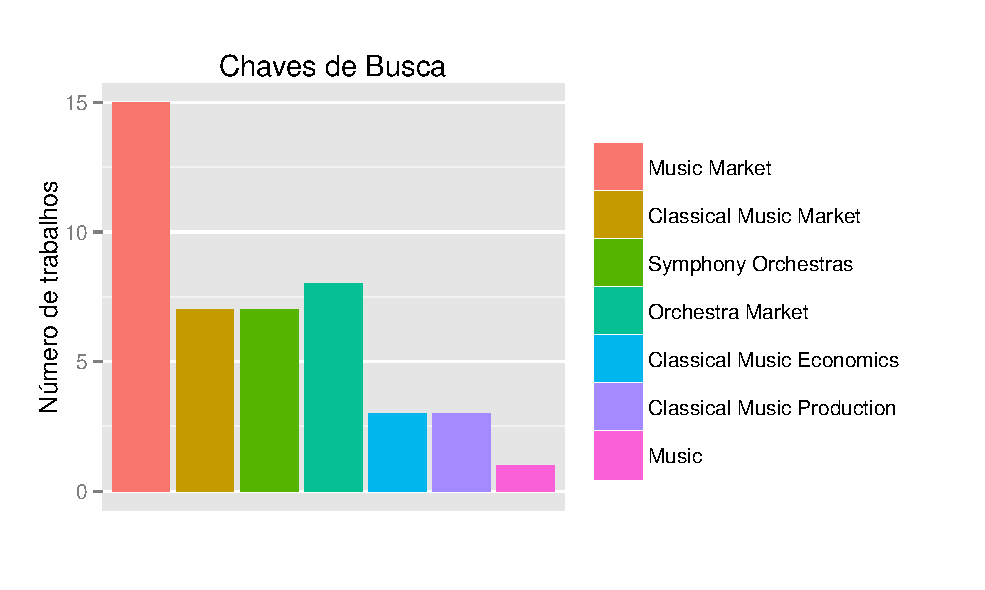
\includegraphics[scale=0.7]{chave.eps}
	%					\legend{Fonte: Dados trabalhados pelo autor}
	%				\end{figure}
	
	%				\begin{figure}
	%					\caption{Tipos de publicação e métodos utilizados por ano}
	%					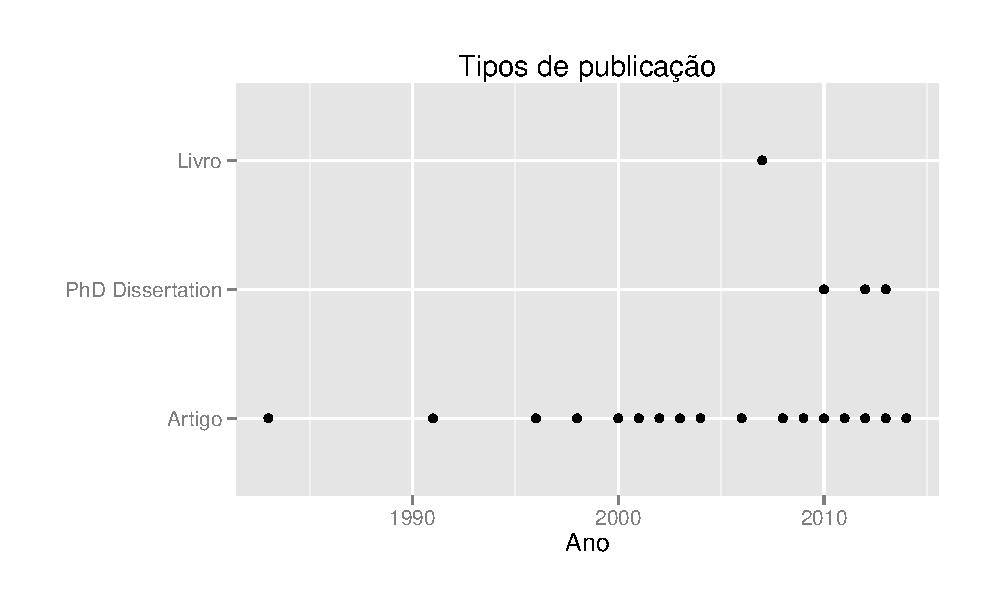
\includegraphics[scale=0.5]{tipopubano.eps}
	%					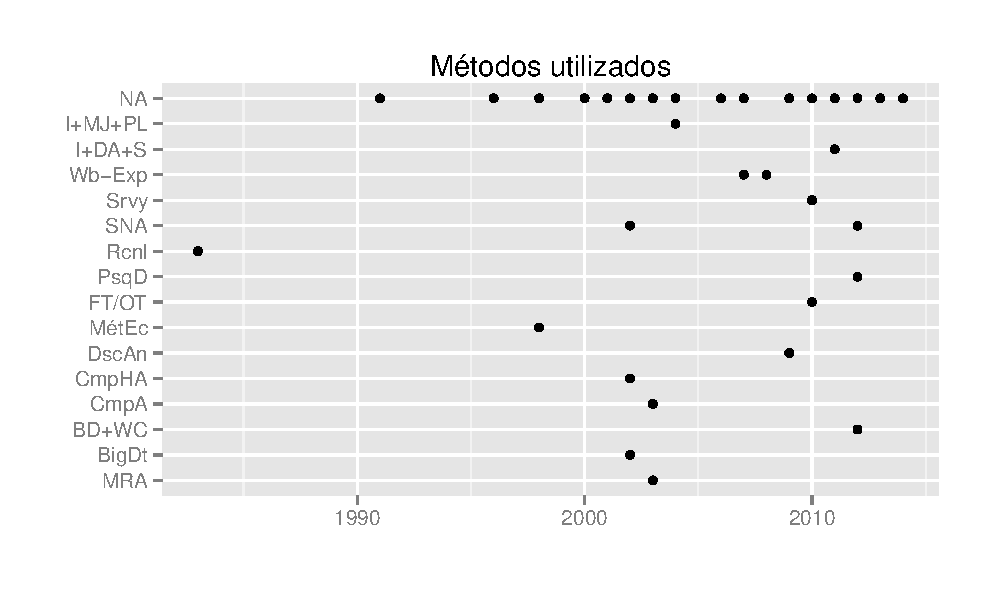
\includegraphics[scale=0.5]{metodoanoab.eps}
	%					\legend{Fonte: Dados trabalhados pelo autor}
	%				\end{figure}
	
	%\begin{figure}
	%	\caption{Métodos utilizados por ano}
	%	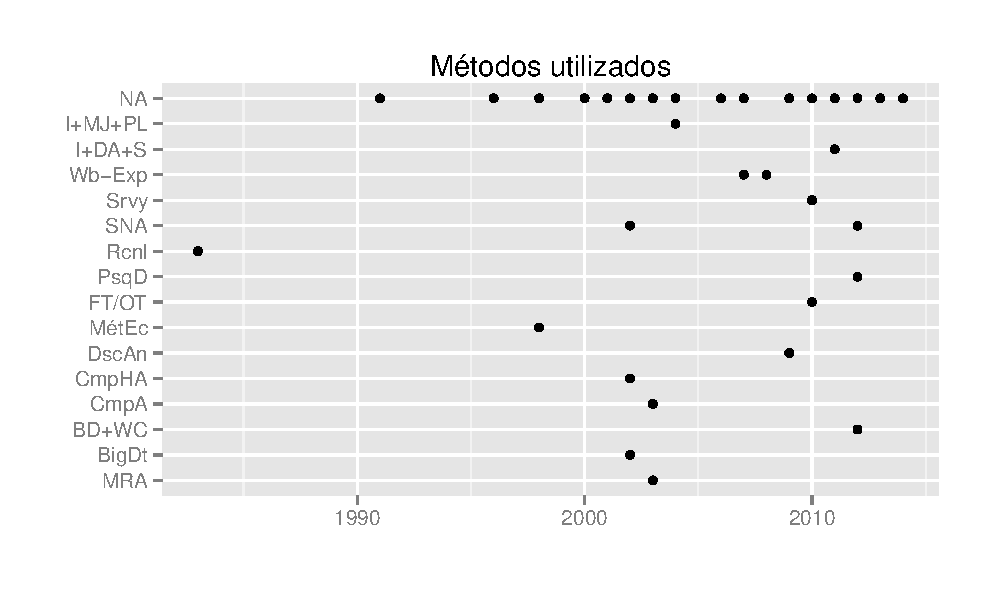
\includegraphics[scale=1]{metodoanoab.eps}
	%	\legend{Fonte: Dados trabalhados pelo autor}
	%\end{figure}
	
	%				\begin{figure}
	%					\centering
	%					\caption{Densidade de publicações por ano}
	%					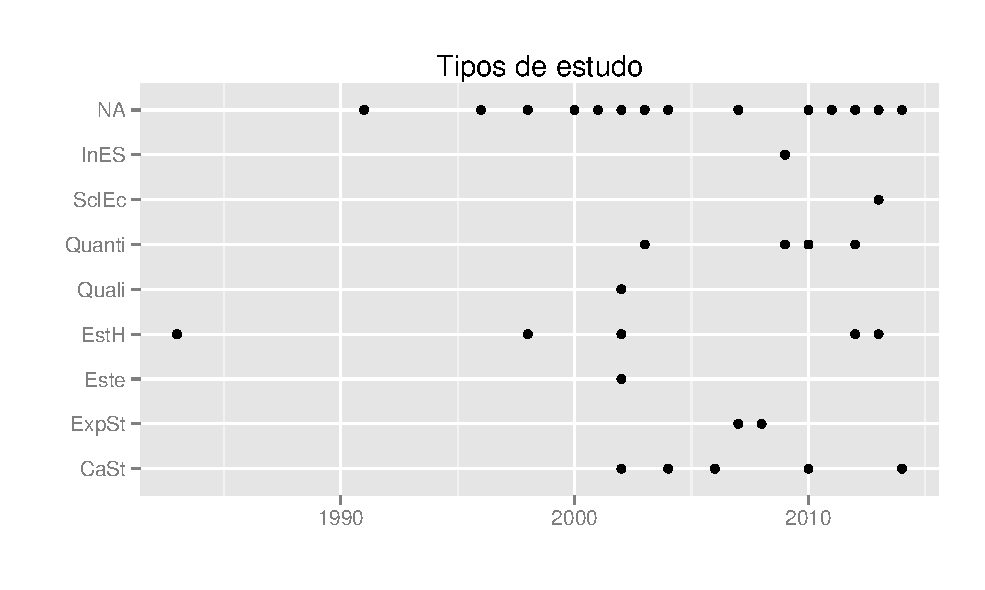
\includegraphics[scale=0.5]{tipoestudoano.eps}
	%					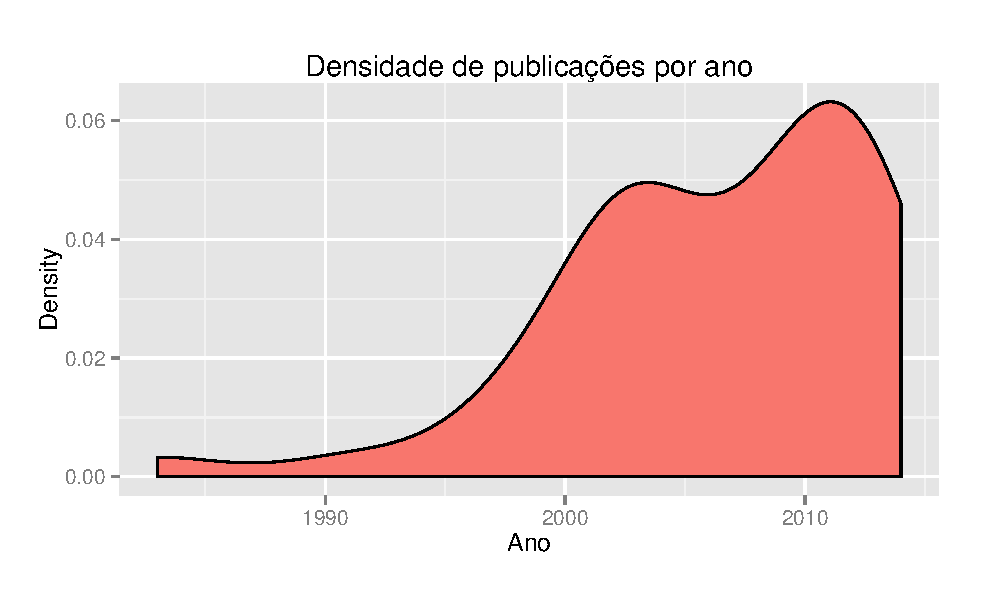
\includegraphics[scale=0.7]{anodensidade.eps}
	%					\legend{Fonte: Dados trabalhados pelo autor}
	%				\end{figure}
	
	%O gráfico de densidade\footnote{Um gráfico de densidade mostra a propabilidade de as observações cairem numa janela de variação ao longo da variável de interesse. Em contraposição ao histograma que mostra uma medida discreta, o gráfico de densidade mostra um contínuo de distribuição dessas probabilidades \cite{lander2014r}.} gerado a partir dos anos de publicação (Figura 3) mostra que, nos trinta e um anos analisados, o campo tem crescido. Este crescimento, entretanto, se deu mais efetivamente nos últimos quinze anos. A densidade das publicações até 1995 é bastante baixa.
	
	%\begin{figure}
	%	\caption{Densidade de publicações por ano}
	%	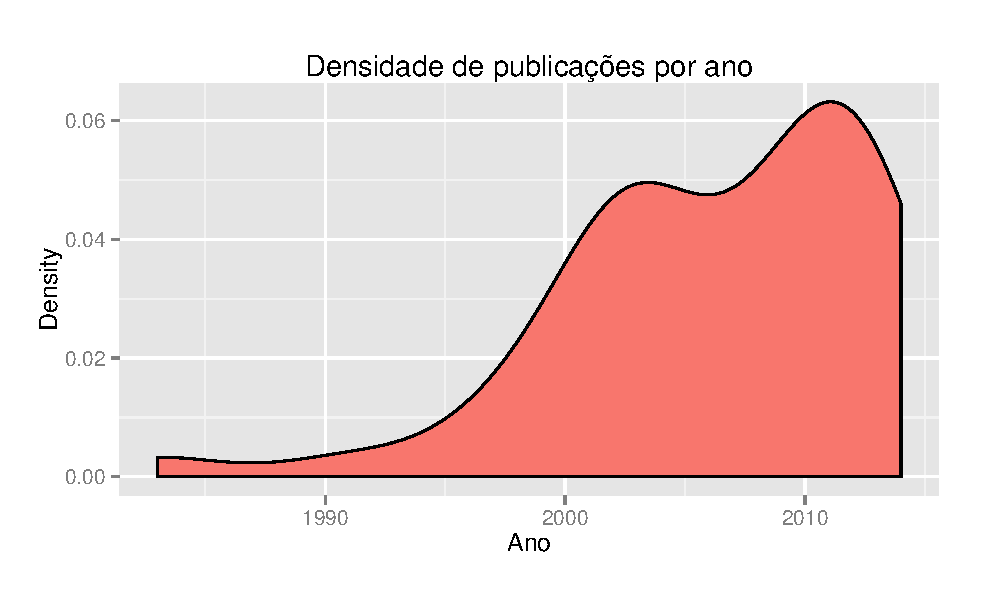
\includegraphics[scale=1]{anodensidade.eps}
	%	\legend{Fonte: Dados trabalhados pelo autor}
	%\end{figure}
	
	%	\section{Perspectivas teóricas e abordagens}
	
	%	Os temas de investigação aparecem nos trabalhos de uma maneira bastante difusa. Encontramos algumas publicações abordando aspectos culturais que influenciam o mercado da música, o mercado de trabalho dos músicos, as relações de gênero e a divisão do trabalho, financiamento e ``patronagem", o consumo da música e as variáveis que o explicam, gosto musical, padrões estéticos, identidade cultural e música nacional/folclórica, história social dos músicos, o ``cânon" do repertório musical, liderança do maestro e participação e satisfação dos músicos, música antiga\footnote{No campo, convencionou-se chamar de música antiga a música escrita até o séc. XVII.}, revolução digital e indústria fonográfica.
	
	%	Percebemos algumas leves polarizações entre os autores expressamente citados nos resumos. Um deles é Bourdieu que, conhecidamente, deixou um vasto trabalho na área de sociologia da arte e do consumo de arte. O nome de Viviana Zelizer aparece relacionado ao de Bourdieu em um resumo consultado. Stigler e Becker são citados num trabalho que argumenta contra a perspectiva econômica neoclássica. Matthew Salganik também aparece nessa bibliografia como autor de dois trabalhos e é citado por mais um indicando novamente atenção ao método experimental na área. No campo, alguns trabalhos tendem a seguir uma perspectiva teórica que privilegia a influência dos aspectos culturais na economia (sociologia econômica). No entanto, não há uma corrente teórica definida perceptível, o que indica que a área não é madura e nem tem uma tradição de pesquisas consolidada.
	
	\chapter{A Construção Social dos Mercados}
	
	Apresentaremos três \textit{frameworks} teóricos que lidam com a emergência dos mercados, a saber, o modelo relacional de Harrison White, o modelo de Fligstein e o conceito isomorfismo tal como desenvolvido principalmente por DiMaggio \& Powell.
	
	\section{O modelo de White}
	
	Para Harrison \citeonline{white2002markets}, os mercados não são dados mas são estruturas sociais que emergem de interações complexas de seus componentes. Essas interações podem acontecer tanto de forma competitiva quanto, argumentamos, de forma cooperativa visando estabilização do mercado e redução do que o professor White chama de ``incerteza knightiana\footnote{Em referência ao economista americano Frank H. Knight.}''.
	
	Sua teoria visa explicar ``como as firmas minimizam incertezas formando um mercado como uma coleção de nichos baseada em sinais observados em seus engajamentos\footnote{(...) how firms minimize uncertanty by forming a market as a collection of niches based on signals observed in their commitments.}'' \cite[p. xiii]{white2002markets}. Em que consiste, portanto, um mercado de produção? A resposta para essa pergunta perpassa duas dimensões. A primeira, já comentada no parágrafo acima, remonta à natureza interdependente de sua estrutura, ou seja, uma emergência a partir das dependências de seus próprios fluxos. A segunda remonta ao seu mecanismo de operação o qual consiste dos engajamentos das diversas firmas em fluxos de produtos nos quais a procura do comprador agregado foi incorporada. Para esse autor ``Os fluxos resultantes de bens ou serviços diferenciados do mercado se dividem entre diversos compradores como opções igualmente boas: \textbf{a disciplina do mercado está centrada na qualidade do produto}\footnote{Resulting streams of differentiated goods or services from the market get split among diverse buyers as equally good options: The market discipline centers on product quality.}'' \cite[p. 1, grifo meu]{white2002markets}. Este ponto é central na caracterização de nosso objeto de estudo. O que seriam, entretanto, disciplinas de mercado?
	
	\citeonline[p. 63]{white2008} indica que ``disciplinas oferecem regras dos jogos que produzem coordenação em tarefas em um mundo que, do contrário, seria caótico\footnote{Disciplines offer rules of the games that yield coordination in tasks in an otherwise messy world.}''. As disciplinas permitem ações conjuntas dando ordem aos laços traçados entre identidades em rede. Cada disciplina possui um tipo de processo que agrega a ação conjunta. Elas possuem ainda um ordenamento de valor específico pelo qual a estrutura se organiza hierarquicamente (por isso, podemos entender as disciplinas também como um sistema local de status). Dentre os tipos ideais de disciplinas elencadas pelo autor, aquela que se aplica aos mercados é chamada de \textit{interface}. Seu processo típico é o \textit{engajamento} que gera fluxos produtivos. O valor distintivo típico desse tipo de disciplina é a \textit{qualidade}.
	
	No caso dos mercados de produção, as firmas engajam fluxos de produtos direcionados ao comprador agregado que são percebidos na interface do mercado como igualmente bons. O distintivo social, o ordenador de valor nessa estrutura, é a qualidade.
	
	Como se articulam os mercados? Para \citeonline{white2002markets}, algumas distinções básicas precisam ser feitas para entendermos sua estrutura. A primeira delas concerne a distinção entre \textit{downstream} e \textit{upstream}\footnote{Pela grande dificuldade em traduzir esses termos, optamos por mantê-los conforme o idioma original. Uma tentativa de tradução pouco elegante poderia ser feita como ``fluxos para baixo'' e ``fluxos para cima''.}, ou seja, os fluxos de produtos engajados pelo produtor em direção ao comprador agregado e a demanda desse comprador agregado o qual é incorporada nos produtos. Essa distinção gera uma segunda distinção concernente a três possíveis papeis para as firmas num mercado, a saber, fornecedor, produtor e comprador. Cada mercado possui uma orientação \textit{upstream} ou \textit{downstream}. Segundo o autor, ``os produtores não estão imbricados em um mercado, como o sociólogo Mark \citeonline{granovetter2007acao} argumentaria; eles de fato constituem a interface do mercado como um set de suas percepções e escolhas\footnote{Producers are not just embedded in a market, as the sociologist Mark Granovetter (1985) [na citação original] would argue; they actually constitute the market's interface in, and as the set of, their perceptions and choices.}'' \cite[p. 8]{white2002markets}. A constituição da interface do mercado se dá em direcionamento à origem percebida de risco. Nesse ponto, para White, reside a fraqueza da teoria econômica ortodoxa.
	
	Ora, a teoria econômica ortodoxa oferece várias tentativas de modelagem de mercados empíricos/realísticos e, para isso, ancora-se em várias asserções provenientes do senso comum. Muito embora esse corpo de conhecimento possua modelos econométricos sofisticados, ele reside muito próximo do senso comum. Entretanto, ao abordar fluxos de produtos em rede num ambiente realístico, a teoria econômica ortodoxa abandona seus modelos, sejam eles realísticos ou de senso comum, e se atém à ficção da competição perfeita. Para \citeonline[p. 9]{white2002markets} ``um enorme custo dessa ortodoxia tem sido a infiltração desapercebida de noções de competição pura na pesquisa de economistas práticos\footnote{One great cost of this orthodoxy has been the unacknowledged infiltration of notions of pure competition into practical economists' research.}''. Do mesmo modo, a sociologia também tem relutado em incorporar os achados da teoria econômica em tentativas de construir críticas mais gerais à influência econômica nos processos sociais a partir das pesquisas de mercados específicos.
	
	Como, então, podemos entender a estabilização de uma interface de mercado? Que propriedades dela podem sucumbir à ``incerteza knightiana'' que atua contra seus membros?
	
	\subsection{Estabilizando a ``incerteza knightiana''}
	
	Transações num mercado tem mais a ver com interações repetitivas do que com momentos únicos. Desse modo, o volume de fluxos de produtos em um mercado pode funcionar como um sinalizador para os produtores sobre os engajamentos. Nas palavras de White:
	
	\begin{citacao}
		Cada um [produtor] pode se orientar em direção a um nicho pelo tamanho que é apropriado à avaliação do mercado de sua própria qualidade comparada à de seus companheiros que também se orientação aos nichos: o mercado como uma construção social conjunta\footnote{Each can orient to a niche by the size that is appropriate to the market's assessment of its quality compared to that of its fellows, who also are orienting to niches: the market as a joint social construction.}. \cite[p. 10]{white2002markets}
	\end{citacao}
	
	Atrelado à interface do mercado está a noção de qualidade que, embora seja comumente tomada por uma característica inerente aos produtos, emerge das interações entre julgamentos tanto de produtores quanto de compradores. Desse modo,
	
	\begin{citacao}
		É uma noção dual de qualidade diferencial referente tanto a produto como a produtor que se torna estabelecida como o centro em volta do qual um conjunto de solos sólidos\footnote{\citeonline{white2008} caracteriza os \textit{footings} ou solos sólidos como definições compartilhadas da vida social sobre a qual os indivíduos orientam sua ação e sua interpretação da ação do outro.} [\textit{footings}] para produtores pode se reproduzir como solos sólidos em um perfil de mercado conjunto. Os dois lados, compradores e produtores, exercem pressões concorrentes no formato desse perfil, pressões que são correlacionadas com suas respectivas discriminações de qualidade\footnote{(\dots) it is dual notions of differential quality, referent both to product and to producer, that become established as the core around which a set of market footings for producers can reproduce itself as footings in a joint market profile. The two sides, buyers and producers, exert contending pressures on the shape of this profile, pressures that correlate with their respective discriminations of quality.}. \cite[p. 10]{white2002markets}
	\end{citacao}
	
	Cada produtor busca diferenciar seu produto e ao mesmo tempo reconhece um sistema de diferenciação  -- o índice de qualidade -- para sua versão de um produto no mercado. Nesse contexto, as escolhas interagem com influência e calibram os engajamentos repetidos de fluxos de produção e de pagamentos. Essa interação entre escolhas pressupõe um mínimo de comparabilidade o que é obtido de uma forma mais simples numa ordem linear de precedência. ``A reputação num ordenamento individual é a moeda de disciplina para mercados de produção'' \cite[p. 10]{white2002markets}, o que se torna difícil de sustentar com muitos participantes devido às nossas limitações cognitivas e de percepção. 
	
	
	\subsection{O mecanismo por trás da produção}
	
	Os engajamentos de fluxos de produtos estão alinhados, de acordo com \citeonline[p. 12]{white2002markets}, a nove fenômenos. São eles:
	
	\begin{enumerate}
		\item um \textit{pequeno número} reconhecido de firmas que constituem uma linha negócios;
		\item uma \textit{identidade} relacionada àquele mercado específico;
		\item um ordenamento \textit{desigual} entre firmas incluindo sua distribuição de lucros e volume de fluxos de produtos engajados no mercado;
		\item as firmas visam \textit{lucro} e não se engajam, conforme a teoria econômica ortodoxa, em um sistema de ``soma zero'';
		\item se as condições permitem o aumento da produção, espera-se que o custo unitário diminua gerando \textit{maiores retornos};
		\item em algumas linhas de negócios, reconhecimento de qualidade superior de um produto exige custos estruturais menores do que outros produtos de qualidade reconhecidamente inferior gerando \textit{retornos perversos};
		\item \textit{monopólios} são fenômenos extremamente \textit{raros};
		\item há um \textit{ciclo de vida} reconhecido dos produtos num mercado;
		\item o \textit{desengajamento} (\textit{decoupling}) ocorre de acordo com variabilidades e caminhos do mercado, não necessariamente por oferta e demanda.
	\end{enumerate}
	
	Esses fenômenos são explicáveis entre si e atravessados por um modelo operacionalizado segundo parâmetros específicos. Nos deteremos agora nesse modelo desenvolvido por \citeonline{white2002markets}.
	
	O modelo parte do pressuposto fundamental de que qualidade e identidade não emanam um do outro mas produzem um ao outro nas interações entre as firmas num mercado. A qualidade é aqui entendida como uma construção social e não como um atributo evidente.
	
	
	\subsection{A racionalidade do modelo}
	
	Chamemos o retorno total recebido por um volume de produtos de \textit{valor} (\textit{worth}). Seja  $W(y)$ o valor do volume $y$. Basicamente, o perfil do mercado pode ser inferido a partir da observação do comportamento dos pares volume-valor (Figura \ref{white_1.2}). 
	
	\begin{figure}[ht]
		\centering
		\caption{Um perfil Retorno X Volume}
		\label{white_1.2}
		\includegraphics[scale=1]{white_1_2.png}
		\fonte{Adaptação de \citeonline[p. 15]{white2002markets}}
	\end{figure}
	
	A curva da figura \ref{white_1.2} é facilmente estimada por um analista de negócios como um guia para um perfil adequado dentro desse mercado. Esse perfil disciplina os engajamentos de cada firma quanto ao volume visando um resultado ótimo de Retornos X Custos. A qualidade se vê refletida nesse perfil e isso se dá sem a necessidade de um índice explícito. As definições da vida são incorporadas em um ordenamento de qualidade o qual perpassa o discurso vigente num domínio em rede. Esse ordenamento que condiciona a formação de laços na rede é percebido em termos de prestígio e combina qualidade de consumo e relações de concorrência \cite{white2002markets}.
	
	Os esforços de uma firma refletidos em sua estrutura de custos tendem a ser refletidas em avaliações do comprador agregado. Essa correlação provê uma base para o ordenamento da qualidade percebida, a saber, um ordenamento linear suficiente para embasar o perfil do mercado. Mas qual é a relação entre os volumes engajados e a qualidade percebida? Isso depende da linha de negócio.
	
	\citeonline{white2002markets} explica, tirando o foco da empresa que atua como compradora e depositando no comprador final -- indivíduo -- e sua percepção de qualidade, que:
	
	\begin{citacao}
		Às vezes, um $y$ grande traz a conotação de maior qualidade como no setor de refrigerantes, mas por outro lado, pode implicar baixa qualidade, como no setor de vinhos. Portanto, a frequência com a qual compradores encontram um \textit{output} de um produtor pode sinalizar coisas diferentes entre formas diferentes de perfil. Como alguns bens monopolizam o espaço nas estantes [de supermercado], mães mais ricas do subúrbio bem como as mães ricas da região Leste em Manhattan, fogem deles já que é isso o que as pessoas comuns estão comprando. Para outros bens que recebem alta exposição nos comerciais, é precisamente isso que esses compradores compram. Afinal de contas, o fato de que todos estão comprando isso confirma que este é o melhor\footnote{Sometimes, a large $y$ connotes higher quality, as in the soda pop industry, but at other times, lower quality, as in the wine industry. So the frequency with which buyers encounter a producer's output (\dots) can signal different things across different shapes of profile. As some goods monopolize shelf space, wealthier suburban mothers, like wealthy East Siders in Manhattan, shy away from them, since they are what the average person is buying. For other goods that receive high exposure in advertising, that's precisely what these shoppers buy. After all, the fact that everyone else is buying it confirms that it's the best.}. \cite[p. 15]{white2002markets}
	\end{citacao}
	
	O ordenamento da qualidade, portanto, envolve um contexto social onde as empresas possuem uma distribuição prévia de prestígio que mescla sua reputação com a de seus produtos. Fluxos de informação são centrais no mecanismo de reprodução de um mercado de produção. Informação útil ao produtor, entretanto, não precisa coincidir com a informação formulada por outros. ``Quando possível para os atores usarem informações lidas das ações de outras, chamamos essa informação de \textit{sinal}. Engajamentos anteriormente feitos são em si mesmos sinais lidos como perfil pelos produtores\footnote{When it is possible for actors to make use of information read from the doings of others, let's call this information a \textit{signal}. Fulfilled prior commitments are themselves the signals read off as profile by the producers.}'' \cite[p. 16]{white2002markets}.
	
	White resume o mecanismo dos mercados de produção da seguinte maneira:
	
	\begin{citacao}
		Um mercado de produção se forma entre produtores e portanto consiste de uma interface conjunta entre eles ao confrontarem incertezas do outro lado da interface. Essa interface é energizada pela rivalidade entre seus pares produtores, todos buscando compradores para seus fluxos contínuos de produção em quantidades ótimas para suas estruturas de custo individuais. Os produtores sinalizam uns para os outros através de um perfil ao longo de seus engajamentos de produção\footnote{A production market forms around and thus consists in a joint interface between producers confronting uncertainty from the other side of the interface. This interface is energized by rivalry among its peer producers, all seeking buyers for their continuing streams of production in amounts optimal for their individual cost structures. The producers have come to signal each other through a profile across their production commitments.}. \cite[p. 27]{white2002markets}
	\end{citacao}
	
	Concentremos nossa atenção aos aspectos formais do modelo de White com relação ao ordenamento de produtores em termos de estrutura de custos e de satisfação com transações.
	
	\subsection{Índice de qualidade -- estrutura de custos}
	
	EXPLICAR\ldots (White, p. 28 em diante)
	
	O lado do produtor -- custos:
	
	\begin{equation}
	\label{eq-custos}
	C(y, n) = q \cdot y^c \cdot n^d
	\end{equation}
	
	O lado do comprador -- qualidade:
	
	\begin{equation}
	\label{eq-qualidade}
	S(y, n) = r \cdot y^a \cdot n^b
	\end{equation}
	
	
	
	\section{O modelo de Fligstein}
	
	Neil \citeonline{fligstein2002architecture} traça uma teorização sobre a emergência e funcionamento dos mercados ligeiramente diferente da que vimos em White. Fligstein também leva em conta uma estrutura relacional onde firmas interagem entre si e com o comprador generalizado visando a estabilização do mercado (e consequente subsistência de todos). A grande diferença fica por conta da participação do Estado. Enquanto White não tece grandes considerações acerca do papel estatal na emergência e funcionamento dos mercados de produção, Fligstein elabora seu esquema teórico identificando a estrutura do Estado como central para o desenvolvimento dos mercados. Por que Estados? - pergunta Fligstein. O próprio autor responde que ``À medida que a possibilidade de padrões de interação complexos na esfera da troca econômica se expandem, os atores se mostraram incapazes de prover regras para si mesmos\footnote{As the possibility for complex patterns of interaction in the sphere of economic exchange has expanded, actors have proven incapable of providing rules for themselves.}'' \cite[p. 27-8]{fligstein2002architecture} e, portanto, recorrem ao Estado como provedor de regras para que o jogo econômico funcione de maneira justa.
	
	\citeonline{fligstein2002architecture} concebe os mercados como ``campos'', arenas sociais onde vendedores e compradores se encontram. Essas arenas obedecem a quatro tipos puros de regras para a produção e reprodução de sua estrutura, quais sejam:
	
	\begin{enumerate}
		\item direitos de propriedade;
		\item estruturas de governança;
		\item regras de troca e
		\item concepções de controle.
	\end{enumerate}
	
	Direitos de propriedade são, segundo o autor, condição \textit{sine qua non} de existência de mercados uma vez que definem as relações entre aqueles que possuem algo e os demais estabilizando o mercado. ``Os direitos de propriedade funcionam, portanto, para produzir duas formas de estabilidade: a definição de relações de poder entre constituintes dentro e fora das firmas e sinalizar a outros quem essas firmas são\footnote{Property rights thus function to produce two forms of stability: defining the power relationships between constituencies in and around firms, and signaling to other firms who firms are.}'' \cite[p. 34]{fligstein2002architecture}.
	
	Estruturas de governança são estruturas de regras que definem relações competitivas e cooperativas entre firmas além de sua organização interna. Elas podem aparecer na forma de leis ou normas sociais.
	
	As regras de troca definem quem pode se engajar em transações comerciais com quem bem como suas condições. As regras abrangem pesos, padrões comuns, fretagem, cobrança, seguro, trocas financeiras e a firma de contratos. ``As regras de troca ajudam a estabilizar os mercados assegurando que as trocas ocorram sob condições que se aplicam a todos\footnote{Rules of exchange help stabilize markets by ensuring that exchanges occur under conditions that apply to everyone.}'' \cite[p. 35]{fligstein2002architecture}. Alguns dos tratados comerciais internacionais mais recentes como o GATT (\textit{General Agreement of Tariffs and Trade}) focam na harmonização das regras de troca.
	
	``Concepções de controle refletem acordos específicos de mercado entre atores em firmas sobre princípios de organização interna (\dots), táticas de competição ou cooperação (\dots), e a hierarquia ou o ordenamento de status das firmas num dado mercado\footnote{Conceptions of control reflect market-specific agreements between actors in firms on principles of internal organization (\dots), tactics for competition or cooperation (\dots), and the hierarchy or status ordering of firms in a given market.}'' \cite[p. 35]{fligstein2002architecture}. São, em sua essência, produtos histórico-culturais.
	
	Para Fligstein, a entrada de países em sistemas capitalistas ``empurra'' os Estados a uma posição regulatória com relação aos quatro tipos acima mencionados. No exercício regulatório, os Estados produzem normativas culturais que determinam o processo de estruturação da ação econômica. Esse exercício é contínuo. Constantemente os Estados lidam com situações de crise e com o \textit{lobby} das empresas clamando por intervenção estatal. Os rumos que os mercados tomam estão diretamente relacionados a dois fatores: (1) a capacidade de intervenção, regulação e mediação do Estado e (2) o poder de organizações privadas para influenciar os termos de intervenção.
	
	O Estado tem ainda um papel fundamental no financiamento da inovação. Segundo \citeonline{fligstein2002architecture}
	
	\begin{citacao}
		Os governos nas sociedades industriais tem um papel importante quanto ao investimento e mediação da luta de classe. As ações dos empresários e empreendedores são enquadradas em torno dessas formas de estabilidade. Eles podem criar novos setores usando a ajuda do governo para investir em tecnologias arriscadas. Eles podem diversificar os riscos em suas firmas para produzir identidades estáveis para as firmas\footnote{Governments in industrial societies play a role in investment and mediating the class struggle as well. The actions of managers and entrepreneurs are framed around these forms of stability. They can create new industries using government support to invest in uncertain technologies. They can diversify their risks in their firms to produce stable identities for firms.}. \cite[p. 62]{fligstein2002architecture}
	\end{citacao}
	
	
	

		
		

	
	
	
	
	
	
	\chapter{A Socioeconomia da Arte}
	
	\begin{comment}
	
	O presente trabalho se insere numa tradição de pesquisa conhecida como a ``Nova Sociologia Econômica'' cuja origem remete ao ``surgimento do debate acadêmico sobre a inclusão de uma perspectiva genuinamente social na economia\footnote{ (…) the opening up of the academic debate about the economy to include a genuinely social perspective.}'' \cite[p. 1]{swedberg1992introduction}. A nova sociologia econômica parte das propostas centrais de que `` 1) a ação econômica é uma forma de ação social; 2) a ação econômica é situada socialmente; e 3) as instituições econômicas são construções sociais'' \cite[p. 6]{swedberg1992introduction}. Desse modo, uma perspectiva sociológica possibilitaria enxergar fatores relacionais que ajudam a responder a perguntas clássicas da economia além de tornar o estudo mais próximo da realidade mesmo não tendo modelos tão elegantes e nem lógica tão consistente em comparação à economia \cite{hirsch1987dirty}. A nova sociologia econômica está preocupada com elementos contextuais das trocas econômicas, analisar como as interações entre os atores fazem emergir um mercado e como essas interações regulam e controlam os mercados. 
	
	O paradigma econômico neoclássico desenvolve-se em contraposição à economia política de Adam Smith, Karl Marx e David Ricardo: esta baseava-se na perspectiva da produção enquanto aquela, no lado do consumo.
	
	Os principais teóricos relacionados à revolução marginalista são Stanley Jevons, Léon Walras e Carl Menger. Esse novo paradigma recebeu o nome de marginalista pelo fato de assumir o princípio da margem de lucro desenvolvido por Ricardo em sua economia da renda da terra. Assume-se também um comportamento racional do agente (\textit{homo economicus}) sempre objetivando o aumento da função de utilidade marginal. Para Jevons o termo utilidade degisna ``a qualidade abstrata que torna um objeto apropriado para nossos fins, caracterizando-o como um bem. Tudo o que é capaz de gerar prazer ou evitar sofrimento \textit{pode} possuir utilidade'' \cite{jevons1996teoria}.
	
	O conceito de utilidade está sustentado na teoria utilitarista conforme proposto por Jeremy Bentham: ``A Natureza (...) colocou a humanidade sob o governo de dois mestres soberanos: \textit{o sofrimento e o prazer}. Cabe a eles indicar o que devemos fazer, assim como determinar o que faremos'' \cite[p. 59]{jevons1996teoria}. Desse modo, a utilidade marginal de um bem é a sua capacidade de suprir alguma necessidade humana maximizando a sensação de prazer ou suprimindo o sofrimento. A utilidade, porém, não é uma qualidade intrínseca aos objetos. ``Define-se melhor como \textit{uma circunstância das coisas} que surge da relação destas com as exigências do homem'' \cite[p. 73]{jevons1996teoria}, sendo algo subjetivo em sua concepção, um estado de satisfação psicológica. Daqui tira-se a principal diferença do pensamento dos marginalistas em relação ao pensamento da economia política: o preço dos bens é derivado do calculo infinitesimal das pequenas quantidades de prazer e dor que podem proporcionar, de sua raridade ou escassez relativa e não do valor-trabalho empregado em sua produção. Segundo \citeonline[p. 109]{walras1996compendio} ``\textit{Os preços correntes, ou preços de equilíbrio, são iguais às relações entre raridades.} Ou seja (\ldots): \textit{Os valores de troca são proporcionais às raridades}''. Interessantes notarmos que, apesar do conceito de utilidade trabalhar no nível subjetivo de satisfação, há um grande esforço de formalização matemática do cálculo de utilidade.
	
	\begin{citacao}
	É claro que, se a Economia deve ser, em absoluto, uma ciência, deve ser uma ciência matemática. (\ldots) acreditando que as quantidades com as quais lidamos devem estar sujeitas a variação contínua, não hesito em usar o ramo apropriado da ciência matemática, não obstante envolva a consideração ousada das quantidades infinitesimais. A teoria consiste na aplicação do cálculo diferencial aos conceitos familiares de riqueza, utilidade, valor, procura, oferta, capital, juro, trabalho e todas as outras noções quantitativas pertencentes às operações cotidianas dos negócios. Como a teoria perfeita de quase todas as outras ciências envolve o uso daquele cálculo, não podemos, então, ter uma verdadeira teoria da Economia sem seu auxílio. \cite[p. 48]{jevons1996teoria}
	\end{citacao}
	
	A unidade de análise característica da economia neoclássica é o indivíduo ou a empresa e o mecanismo de coordenação social por excelência é o preço. O paradigma neoclássico pressupõe a livre concorrência, ou seja, o mercado perfeito. Segundo Jevons
	
	\begin{citacao}
	A concepção teórica de um mercado perfeito se confirma mais ou menos completamente na prática. Em qualquer grande mercado, é trabalho dos corretores organizar a troca de forma que qualquer compra seja feita com o mais completo conhecimento das condições de comércio. Todo corretor se esforça para obter o melhor conhecimento das condições de oferta e procura e do primeiro indício de qualquer mudança. Ele está em ligação com quantos outros corretores for possível, de forma a ter o mais amplo campo de informação e a maior oportunidade de fazer trocas convenientes. Somente dessa maneira é que a todo momento um preço de mercado preciso pode ser definido e variado, de acordo com as frequentes notícias capazes de afetar compradores e vendedores. Um consenso geral é estabelecido pela mediação de um corpo de corretores, e o estoque de todo vendedor ou a demanda de todo comprador são levados ao mercado.\textit{A informação ampla e constante é a própria essência do comércio.} Portanto, um mercado é teoricamente perfeito apenas quando todos os comerciantes tem perfeito conhecimento das condições de oferta e procura, e da relação de troca consequente; e em qualquer momento nesse mercado, como veremos agora, poderá haver apenas uma relação de troca de um bem homogêneo. \cite[p. 98, grifo meu]{jevons1996teoria}
	\end{citacao}
	
	Conforme apontado pelo autor, o amplo conhecimento das condições de mercado é condição necessária para o mercado autorregulado.
	
	O comportamento racional dos indivíduos assumido pelos marginalistas pode ser exemplificado na concepção de Jevons de coletivos econômicos. Os coletivos econômicos são agregados de indivíduos. Para ele a expressão comunidade comercial designa ``de modo geral, qualquer comunidade tanto de compradores como de vendedores'' \cite[p. 99]{jevons1996teoria}, as quais tem influência conjunta no mercado. ``A comunidade comercial pode ser o indivíduo isolado, num caso; podem ser todos os habitantes de um continente, em outro; podem ser os indivíduos de um ramo de negócios espalhados em país, em um terceiro caso'' \cite[p. 99]{jevons1996teoria}.
	
	Apesar do esforço de Jevons em direção a um maior grau de formalização da economia, é com Walras que a economia atinge o topo da abstração metodológica ao pensar a totalidade da esfera econômica como um sistema autorregulado. O enfoque desse autor é no equilíbrio econômico. A sua preocupação é construir uma base analítica que permita entender o funcionamento de mecanismos de preço na coordenação das trocas econômicas em mercados diversos \cite{carneiro1996apresentacao}.
	
	\begin{citacao}
	A construção walrasiana do equilíbrio geral entende, assim, o sistema de preços competitivos como um mecanismo de incentivos que promove a compatibilidade entre o resultado da ação do poder aquisitivo de cada agente econômico em busca de realizar seus objetivos individuais e as quantidades totais de recursos à disposição da sociedade. \cite[p. 12]{carneiro1996apresentacao}
	\end{citacao}
	
	Segundo \citeonline[p, 38]{steiner2006}, a teoria do equilíbrio de Walras ``parte da ideia de que a representação de conjunto de um sistema econômico deve levar em conta as inter-relações dos diversos componentes do sistema''. Uma mudança de preço de um bem determinado em um mercado tem reflexo em todos os outros mercados porque uma mudança de preços altera tanto a oferta e a demanda de todos os agentes no mercado desse bem, quanto todo o mercado em geral. A partir daí, surgem novas alterações de preços dando origem a um novo equilíbrio, a saber, ``a preços correntes, nenhuma transação é mutuamente vantajosa para os dois agentes'' \cite[p. 38]{steiner2006}. O equilíbrio do sistema, como um todo, é atingido quando toda oferta encontra a sua procura e toda procura, a sua oferta, isto é: 1) quando todos os consumidores podem gastar sua receita segundo suas preferências, 2) quando todas as empresas vendem seus produtos ou serviços cobrindo pelo menos seus custos, 3) quando todos os fatores oferecidos no mercado são utilizados na produção dos bens e serviços sendo que todos os produtos oferecidos são os produtos demandados, e 4) quando os ingressos gastos pelos consumidores são ingressos recebidos pelos consumidores. Para Steiner, a prova da existência de um equilíbrio
	
	\begin{citacao}
	é um resultado formal importante que vai no sentido da intuição smithiana, segundo a qual uma ordem econômica coerente e desejável pode resultar do comportamento egoísta de agentes autônomos. Mas nada permite pensar que esse resultado seja evidente por si mesmo. Os limites da teoria do equilíbrio geral não são menos importantes, sobretudo quando se trata de demonstrar como se efetua a passagem entre os comportamentos individuais e os dados agregados (\ldots), quando se trata de introduzir a moeda (\ldots) ou ainda quando se trata de estudar o processo pelo qual se chega ao equilíbrio. \cite[p. 38-9]{steiner2006}
	\end{citacao}
	
	
	
	
	APROVEITAR A PARTIR DAQUI
	REVISAR!!!!!!!!!!!!!!
	
	Dito de outra forma, o pensamento econômico neoclássico deixa uma pergunta em aberto a partir da qual se desenvolverá boa parte do programa de pesquisa conhecido como ``a nova sociologia econômica'': As condições essenciais para que o mercado se aproxime de seu tipo puro são a liberdade de contratos e a propriedade privada. Entretanto, \textit{estes não são os únicos fatores de estabilização no espaço mercantil.} Quais são os outros fatores ou variáveis sociais que garantem a existência de mercados e preços?
	
	Mark Granovetter foi um dos principais \textit{scholars} a oferecer resposta para essa pergunta. Em suas palavras
	
	\begin{citacao}
		Minha abordagem da sociologia econômica apoia-se em duas proposições sociológicas fundamentais: em primeiro lugar, a ação é sempre socialmente localizada e não pode ser explicada, fazendo-se referência, apenas, aos motivos individuais que possam tê-la ensejado; em segundo lugar, as instituições sociais não brotam automaticamente, tomando uma forma incontornável; elas são construídas socialmente. \apud[p. 27-8]{granovetter1990old}{steiner2006}
	\end{citacao}
	
	A ausência de interferências e a confiança são elementos essenciais de um mercado que, o individualismo radical coloca em xeque. Granovetter, na tentativa de entender as condições de existência dos mercados parte da constatação de que a ação humana costuma ser considerada hipossocializada ou hiperssocializada. Na perspectiva hiperssocializada, concepção que ganhou proeminência a partir dos trabalhos de Parsons \cite{granovetter2007acao}, pensa-se que a desconfiança e as incertezas no mundo dos negócios são afastadas por uma moralidade geral vigente que favorece o clima das trocas. Na perspectiva hipossocializada, de tipo neoinsitucional com seu viés hobbesiano, pensa-se que as instituições, com seu poder de sanção, desencorajam as práticas desleais, fazendo com que sejam mais custosas para os oportunistas. As instituições seriam um substituto funcional para a falta de confiança.
	
	Para Granovetter, a geração de confiança e o controle da deslealdade estão cimentados em duas premissas: são o produto de relações pessoais concretas e das redes nas quais estão inseridos os atores. O fato de preferir negociar com pessoas de conhecida reputação não depende de uma moralidade geral ou do controle vertical de uma instituição. A confiança não é uma propriedade dos agentes do mercado e sim o produto de suas relações.
	
	As relações concretas não podem ser entendidas como um substituto funcional da confiança, de tal forma que sustentem a ordem econômica. As relações sociais penetram com graus diferentes de intensidade os diferentes setores da vida econômica, e sempre são condição necessária, mas não suficiente, do comportamento confiável.
	
	Para entendermos o pensamento de Granovetter, faz-se mister a compreensão de seu projeto epistemológico para a ação social. Para esse autor as ações sociais e econômicas estão imersas (\textit{embedded}) na rede de relações dos atores. Este argumento propõe que ``os comportamentos e as instituições a serem analisados são tão compelidos pelas contínuas relações sociais que interpretá-los como sendo elementos independentes representa um grave mal-entendido'' \cite[p. 3]{granovetter2007acao}.
	
	\begin{citacao}
		A preferência dominante em fazer transações com indivíduos de reputação conhecida implica que poucos estão realmente dispostos a confiar na moralidade generalizada \textit{ou} nos dispositivos institucionais para evitar problemas. Os economistas \textit{notaram} que um incentivo para não enganar o outro é o custo dos danos infligidos à reputação pessoal; mas essa concepção da reputação como uma \textit{commodity} generalizada, um cálculo entre as vantagens e as oportunidades de enganar, representa uma concepção subsocializada. Na prática, recorremos a essas informações generalizadas quando nada melhor está disponível, mas normalmente buscamos melhores informações. Melhor que a afirmação de que alguém é conhecido pela sua honestidade é a informação de um informante confiável que já lidou com esse indivíduo e o considerou honesto. Ainda melhor é a informação das próprias transações que foram feitas com essa pessoa no passado. \cite[p. 12]{granovetter2007acao}
	\end{citacao}
	
	A abordagem de Granovetter se situa num espaço entre a perspectiva hiperssocializada e a perspectiva hipossocializada. ``Diferentemente das duas alternativas ou da posição de Hobbes, essa visão não produz previsões generalizáveis (e portanto improváveis) de ordem ou desordem universal, mas sustenta que cada situação será determinada pelos detalhes da estrutura social'' \cite[p. 15]{granovetter2007acao}. Para esse autor, as relações sociais entre as empresas tem um peso maior na manutenção da ordem da vida econômica do que a hierarquia formal interna \cite{granovetter2007acao}.
	
	Desse modo, o agente econômico é visto aqui como dependente da estrutura formada pela rede de relações contínuas a qual pertence e não mais como um indivíduo racional que faz cálculos de utilidade (tendo toda a informação suficiente para isso) para elaborar sua ação: o \textit{homo economicus}. O sistema econômico é concebido como uma grande rede de relações onde circulam informações, recursos e, de seu funcionamento, emergem crenças, sistemas de status, confiança, sistemas de obrigações e expectativas e sanções sociais que são seus principais reguladores.
	
	Um trabalho emblemático de pesquisa em sociologia econômica visou examinar se os fatores sociais relacionados ao mercado de morangos em \textit{Fontaine-en-Sologne} ``são variáveis residuais por meio das quais poder-se-ia explicar a posteriori as distâncias entre os fatos observáveis e os que o modelo [de mercado perfeito] prevê, ou se eles intervêm em todo o processo das praticas de mercado das mais 'econômicas''' \cite[p. 6]{garcia2003construccao}. Para a autora, a segunda opção é a condizente com a realidade. Ela explica que ``o mercado de \textit{Fontaines} não se criou num vácuo social, mas em oposição a relações já constituídas diante das quais certos indivíduos não se achavam mais suficientemente recompensados'' \cite[p. 33]{garcia2003construccao}. Houveram esforços para superar as relações com corretores, investimentos financeiros em infraestrutura, a criação de uma associação e um investimento psicológico visando produzir a crença no sucesso, consenso e confiança.
	
	\begin{citacao}
		O funcionamento ``perfeito'' do mercado não é efeito de ``mecanismos'' dados ``naturalmente'' (em que pese o paradoxo destes termos), nem decorre de uma ``mão invisível'' restaurada por meio da aplicação do ``laissez-faire, laissez passer'', mas se deve ao trabalho de alguns indivíduos com interesse em que ele viesse a existir e da aceitação dos limites do jogo impostos a todos os demais participantes que também chegaram a se beneficiar de sua existência. Esse mercado deve ser considerado mais como um campo de lutas do que como produto de leis mecânicas e necessárias inscritas na natureza do mundo social, embora algumas vezes desfiguradas por ``fatores sociais''. \cite[p. 35-6]{garcia2003construccao}
	\end{citacao}
	
	\end{comment}
	
	
	
	
	
	
	
	
	
	
	
%	\section{A Economia da Cultura}
	
	\begin{comment}
	
	
	%Epígrafe
	\begin{citacao}
		\textit{Paralelamente ao que ocorre com a declamação do ator, a fala do orador ou a melodia do músico, o trabalho de todos eles morre no próprio instante de sua produção.} Adam \citeonline{smith1996riqueza}, Livro II, cap. 3.
	\end{citacao}
	
	
	Para \citeonline[p. 51]{reis2007economia}, ``a economia da cultura surgiu por iniciativa não da economia, mas da cultura'', ou seja, ``de uma instituição dotada de perspectiva privilegiada da dinâmica cultural''. A autora mostra evidências de uma associação conhecida como Accademia di San Luca em Roma no séc. XV que seria uma precursora dos sindicatos de artistas. Segundo \apudonline{haskett1997mecenas}{reis2007economia}, em 1633 a instituição recebeu autorização para arrecadar tributos dos artistas sendo ou não membros e detinha o monopólio das encomendas públicas. A autora cita ainda o trabalho de \citeonline{vasari2004pittori} que nos dá um panorama de mais de mil páginas sobre as idas e vindas dos artistas europeus de acordo com o fluxo do mercado da época o que, segundo a autora, era muito distante da ideia de senso comum da vida do artista garantida pela solicitude de seus mecenas. A autora mostra que
	
	\begin{citacao}
		Se a associação de obras de arte às classes dominantes, constituindo ao mesmo tempo veículos transmissores de mensagens, símbolo de status e poder e, por que não, prazer estético legítimo, não constitui novidade, a visão do mercado de obras de arte tampouco é invenção de nossos tempos. Porém, a abordagem sistêmica de fluxo e a percepção da necessidade de intervenção do Estado para corrigir distorções de mercado, em prol dos objetivos de política pública, só entrou em cena, como objeto de interesse da economia, na recente década de 1960. \cite[p. 51]{reis2007economia}
	\end{citacao}
	
	Antes de nos determos especificamente à participação (crucial) do Estado na produção da música de concerto, é preciso olhar para o setor numa perspectiva sistêmica mais holística. O economista Paul \citeonline{tolila2007cultura} apresenta uma tipologia interessante do processo de produção nas indústrias culturais a qual chama de ramos de produção. Muito embora esse autor foque a indústria cultural, um nicho de mercado mais amplo e fundamentalmente divergente do setor da música de concerto, acreditamos que o modelo possa ser frutífero para pensarmos o setor aqui investigado por comparação.
	
	\subsection{A tipologia dos ramos de produção}
	
	Para \citeonline[p. 38]{tolila2007cultura}, um ramo de produção, entendido aqui como uma ``sequência de operações que se sucedem desde o tratamento das matérias-primas até a elaboração do produto final'', pode ser dividido em cinco fases. 
	
	A \textit{fase 1} compreende os processos criativos e de concepção de protótipos. Aqui estão contidas a redação de um romance, a composição de uma obra musical ou até mesmo o desenvolvimento do código-fonte de um \textit{software}. A \textit{fase 2} consiste da edição e produção e, segundo \citeonline{tolila2007cultura}, do ponto de vista econômico é a fase-chave das indústrias culturais. ``Ela consiste em assegurar a coordenação da fase `inicial' com o conjunto de fases seguintes para fazer a criação de um artista alcançar um status de `bem cultural' oferecido (e, se possível, vendido) num mercado''. Esta é a fase de maior risco no processo devido aos pesados investimentos necessários. Também por esse motivo, nessa fase envolvem-se comumente atores econômicos de grande porte como grandes empresas ou grupos econômicos.
	
	A \textit{fase 3} é chamada pelo autor de ``fase de fabricação'' e consiste na produção de produtos físicos (CD's, DVD's, Livros, etc.) em 3 etapas, a saber, a fabricação, duplicação industrial e reprodução. Normalmente esta fase compreende atividades subcontratadas pelo gestor responsável pela fase 2. A \textit{fase 4} é denominada ``fase da distribuição'' ou difusão. Aqui, o produto é colocado em circulação nas redes comerciais. Essas atividades assumem grande variabilidade dependendo do ramo em questão (e.g., promoção de catálogos no ramo de livros, custos de comunicação e publicidade no ramo da música). Por fim, a \textit{fase 5} consiste da comercialização pública do produto. Nessa fase podem estar envolvidos tanto varejistas (pequenas livrarias e lojas de discos) quanto o que \citeonline[p. 39]{tolila2007cultura} chama de ``megalojas especializadas em produtos culturais'' como a Fnac ou hipermercados. O autor pondera que
	
	\begin{citacao}
		Na vida econômica concreta do conjunto dos atores envolvidos nessas diferentes fases, ocorrem combinações variáveis de suas relações. A fase 1 é uma fase ``à parte'', o que determina um certo número de desafios econômicos (\ldots). A terceirização da fase 3 continua, mas com a baixa dos custos de produção e a padronização dos processos industriais induzidos pela automação e a robotização ela não apresenta um grande interesse em termos de valor agregado; ao contrário, a competição pode ser muito feroz e centrar-se apenas em nichos muito especializados que permitem os ``pequenos fabricantes'' viverem num mundo em que a corrida aos preços baixos deixa lugar apenas aos industriais capazes de acompanhar o mercado em termos de produtividade, reatividade e tamanho crítico. Alguns grandes, aliás, se concentram em dominar completamente essa fase de maneira interna por razões estratégicas de conduta oligopolista. \cite[p. 40]{tolila2007cultura}
	\end{citacao}
	
	As fases 2, 4 e 5 contém relações mais complexas entre seus atores. A fase de edição e produção (2), é marcada por constantes fenômenos de concentração. Para \citeonline[p. 40]{tolila2007cultura}, isso pode ser explicado pela ``intensidade capitalista hoje requerida nesses setores e pela necessidade de dispor de um catálogo muito diversificado''. A fase 4 apresenta a mesma propensão à concentração por representar ``o meio por excelência de acesso aos mercados e uma forte ferramente de pressão''. 
	
	Segundo \apudonline{stigler1961economics}{tolila2007cultura}, a teoria econômica padrão coloca que o mercado não suporta empresas especializadas em cada uma das fases do ramo na presença de uma indústria. ``Quando as oportunidades de mercado se desenvolvem, a existência de empresas especializadas torna-se possível graças à lógica das especializações de funções e de sua viabilidade e se produzem fenômenos de desintegração vertical no ramo considerado'' \cite[p. 41]{tolila2007cultura}. Para esse autor, as indústrias culturais funcionam do mesmo modo embora assumam também movimentos de integração vertical no sentido inverso, i. e., atores da fase 2 ligando-se diretamente aos da fase 5 ou 4. Isso é provocado pela internacionalização dos mercados e desequilíbrios internos nos níveis nacional e internacional do setor. Para \citeonline{tolila2007cultura}
	
	\begin{citacao}
		A causa fundamental de todos esses movimentos reside \textbf{na necessidade de recuperar ao máximo o valor agregado} nas diferentes fases em que ele se criou e conservar ou aumentar suas capacidades competitivas ou suas posições, sobretudo quando elas são dominantes. Como as indústrias culturais se converteram num setor muito competitivo em que não se pode diminuir muito a incerteza, a competição pelo valor agregado tornou-se regra. \cite[p. 42]{tolila2007cultura}
	\end{citacao}
	
	\textit{O mercado das indústrias culturais, como podemos perceber, se distancia do modelo neoclássico de mercado perfeito ou autorregulado.} Para que um mercado seja perfeito, é necessário que as incertezas seja reduzidas a zero e que todos os atores tenham acesso irrestrito a toda a informação disponível. Esse mercado, contrariando a teoria neoclássica, opera sobre um contexto de incertezas, embora tenha desenvolvido mecanismos para driblá-las como a repetição de um padrão que tem se mostrado eficiente. Para \citeonline[p. 46]{tolila2007cultura} esse comportamento ``é pouco glorioso no plano da inovação artística, mas extremamente rentável em termos financeiros''. 
	
	Como então se estruturam os mercados das indústrias culturais?
	
	Para o economista americano Georges Stigler, o setor ``se estruturou sobre o domínio das grandes empresas (as `majors') em torno das quais vivem e atuam, contudo, uma miríade de empresas pequenas, algumas muito pequenas até'' \cite[p. 43]{tolila2007cultura}. O oligopólio de franjas, como ficou denominado, é definido por uma franja concorrencial dividida em nichos de mercado e que circunda o centro oligopolístico. Segundo \citeonline{tolila2007cultura}, a franja concorrencial, o conjunto de pequenas empresas, caracteriza-se por sua fraqueza e fragilidade. Essas empresas atuam sobretudo na fases 2 (sociedades de produção, selos independentes e editoras independentes) e 5 (salas de arte, pequenos teatros, impressoras especializadas, lojas de discos e livrarias) e tem sua entrada no processo produtivo nas fases em que a dominação do centro não se desenvolve de maneira absoluta. 
	
	Para prosseguirmos, faz-se necessário nos aprofundarmos nas especificidades do bem cultural central para este trabalho, as performances de uma orquestra.
	
	\end{comment}
	
	
	
	\section{A performance musical como produto cultural}
	
	Comecemos estabelecendo algumas diferenças fundamentais entre os bens e mercadorias conforme concebidos tradicionalmente pela teoria econômica e as performances musicais.
	
	As mercadorias são entendidas por meio de quatro critérios objetivos, a saber, suas propriedades físicas (as quais, nesse caso, estão diretamente relacionadas com a qualidade do produto em questão), a data e o local em que ele está disponível e aquilo que condiciona sua entrega num universo certo, i.e., sem incertezas. A qualidade de um bem, nessa perspectiva, pode ser decomposta em uma série de elementos objetivos, i.e., claramente mensuráveis e hierarquizáveis. Além disso, na teoria econômica clássica todo bem é considerado um ``bem privado'' e, portanto, ``exclusivo e rival'' no consumo. Para citar um exemplo, ``um café, um sanduíche, uma camisa, um par de sapatos, uma cadeira, etc., são bens exclusivos porque é possível impedir-me de obtê-los (\ldots); por outro lado, cada um desses bens é de consumo exclusivo porque no momento em que o aproveito, nenhuma outra pessoa pode usufruí-lo'' \cite[p. 29]{tolila2007cultura}. Ora, os produtos culturais, de um modo geral, são não exclusivos; pode-se, por exemplo, admirar um belo edifício histórico na rua sem ter que pagar por isso. Tampouco são rivais no consumo; o prazer de assistir um concerto não é diminuído pela presença de outras pessoas no público.
	
	Esse setor da economia define-se, ainda, pela sua lógica de oferta voltada à produção, ao contrário dos mercados de bens comuns voltados ao consumo. Para \citeonline[p. 32]{tolila2007cultura}, ``essa lógica da oferta caracteriza bem, entre outras, a ação das políticas públicas em termos de investimento, de ajuda e de sustentação das atividades culturais, do patrimônio ao espetáculo ao vivo, e em termos de incentivos às práticas culturais''. De fato, os Estados e coletividades públicas tem demonstrado interesse crescente no setor cultural, o que pode ser verificado através das políticas públicas, das administrações especializadas, da alocação de recursos dirigidos especificamente ao setor e do surgimento de toda uma rede de instituições e profissionais atuantes no setor cultural, grande parte deles financiados por dinheiro público \cite{tolila2007cultura}. Para \citeauthoronline{tolila2007cultura}
	
	\begin{citacao}
		Consequentemente, a atenção das autoridades, dos cidadãos e de seus representantes, foi desenvolvida em duas direções clássicas no contexto das democracias: por um lado, \textbf{o debate público interno} sobre a alocação dos recursos, o valor deles e seu significado, por outro, \textbf{a competição exterior} com os outros Estados pelas questões de mercados e de comércio. Essa segunda direção (\ldots) é inseparável dos dilemas e debates que movimentam atualmente todas as reflexões sobre \textbf{a globalização e a diversidade das expressões culturais}. \cite[p. 71-2]{tolila2007cultura}
	\end{citacao}
	
	Para esse autor, esses dois elementos são constitutivos do valor simbólico atribuído às práticas e ao desenvolvimento cultural à medida que traz relevância ao debate relacionado à identidade e diversidade cultural. O valor simbólico dos bens culturais constitui, para nós, um elemento central na compreensão de nosso objeto de estudo, muito embora, contrariando novamente a teoria econômica clássica, não seja objetivo em sua natureza mas relacional e individual, i.e., só existe à medida que é reconhecido pelo indivíduo no momento de seu consumo. Para que o valor simbólico de um determinado bem seja reconhecido, é necessário que haja estruturas cognitivas apropriadas para a compreensão e fruição do bem, ou seja, esquemas mentais adquiridos por meio da educação artística prévia \cite{bourdieu2003amor}.
	
	As performances musicais possuem ainda uma particularidade quanto à natureza de sua existência na qual reside grande parte das dificuldades metodológicas que as cercam. \citeonline{tolila2007cultura} explica:
	
	\begin{citacao}
		O que é a música? A partitura escrita? Não. Os músicos que formam a orquestra? Não. O regente? Também não. Na verdade, é quase impossível definir a música como uma ``coisa'' (uma mesa, uma cadeira, uma casa, etc.) pois ela só existe de fato no momento em que é ouvida, isto é, em uma relação com o ouvinte\footnote{Para o autor, ``na verdade, no mundo social, o modo real de existência da maioria dos fenômenos é o da relação entre seres humanos'' \cite[p. 110]{tolila2007cultura}. Curiosamente, nessa premissa se baseia todo o paradigma neoestrutural na sociologia conhecido também como ``perspectiva relacional'' ou ``teoria das redes sociais''.}. \cite[p. 109]{tolila2007cultura}
	\end{citacao}
	
	Desse modo, a música (bem como a dança e o teatro, por exemplo) assume um modo especial de existência que envolve a participação de todos os elementos ou atores supracitados, a saber, partitura, músicos, regente, etc., na construção de sua materialidade que só existe (e portanto só é possível de ser consumida) no momento da escuta. Segundo \citeonline[p. 54]{benhamou2007economia} ``a concorrência assume a forma paradoxal de uma competição entre instituições que oferecem bens únicos e efêmeros'' onde o comportamento dos atores econômicos tende a monopólios discriminatórios. Para essa autora, o setor é caracterizado por uma fragilidade constante devido a elevações periódicas de custos e à quase-ausência de reservas de produtividade. De fato, como veremos, o paradigma vigente, no que tange a teoria econômica das performances ao vivo, aponta para um inevitável estado deficitário.
	
	\section{O modelo de Baumol e Bowen -- a ``doença dos custos''}
	
	William Baumol e William Bowen empreenderam, sob encomenda da Fundação Ford em 1965, uma pesquisa visando diagnosticar a situação econômica dos teatros da Broadway \cite{benhamou2007economia}. Seus achados são até hoje considerado válidos. Para \apudonline{baumol1966performing}{benhamou2007economia} a economia divide-se em dois setores, o setor 1 (arcaico) e o setor 2 (progressista). O setor arcaico não apresenta possibilidades de gerar ganhos de produtividade enquanto o setor progressista gera ganhos de produtividade a partir de inovações, de economias de escala e da acumulação de capital. A performance ao vivo faz parte do setor arcaico e isso se deve à posição que nele ocupa o trabalho. Para \citeonline{benhamou2007economia}
	
	\begin{citacao}
		O trabalho é um elemento constitutivo do produto final: não se poderia substituí-lo sem desnaturar o produto. Não se poderia, por exemplo, substituir um dos instrumentistas de um quarteto de cordas por uma gravação\ldots Ora, os salários são iguais aos do setor progressista, devido à fluidez do mercado de trabalho; a consequência é um aumento permanente dos custos relativos do espetáculo ao vivo, que somente uma elevação dos preços das entradas pode compensar, com o risco de reduzir a demanda e as receitas. 
	\end{citacao}
	
	O modelo de \apudonline{baumol1966performing}{benhamou2007economia} baseia-se nas três hipóteses que se seguem:
	
	\begin{enumerate}
		\item A economia divide-se em dois setores, arcaico e progressista. No setor arcaico, onde reside a performance ao vivo, a produtividade do trabalho é constante ou aumenta pouco e a quantidade de trabalho não pode ser diminuída sem desnaturar o produto. Sendo $L_{1,t}$ o volume de trabalho empregado no setor 1 no momento \textit{t} e \textit{a} um valor constante, a quantidade de produto no setor 1 no momento \textit{t} ($Y_{1,t}$) é obtida por $$Y_{1,t} = aL_{1,t}$$
		
		Sejam $Y_{2,t}$ e $L_{2,t}$ respectivamente a quantidade de produto do setor progressista no momento \textit{t} e o volume de trabalho empregado no setor 2 no momento \textit{t}, seja r a taxa de aumento da produtividade do trabalho e \textit{b} uma constante, a quantidade de produto no setor é obtido por $$Y_{2,t} = bL_{2,t}[1+r]^t $$
		
		\item Os custos de produção, comparados somente com os custos salariais (\textit{W}), evoluem no mesmo ritmo e sentido que a produtividade no setor progressista, isto é, $W_{1,t} = W_{2,t} = W_t = W[1+r]^t$. Os custos relativos de cada setor são, portanto, dados por
		$$C_1 = \frac{W_tL_{1,t}}{Y_{1,t}} = \frac{W(1+r)^tL_{1,t}}{aL_{1,t}} = \frac{W(1+r)^t}{a}$$
		$$C_2 = \frac{W_tL_{2,t}}{Y_{2,t}} = \frac{W(1+r)^tL_{2,t}}{bL_{2,t}(1+r)^t} = \frac{W}{b}$$
		
		Tem-se, então, que o custo por unidade de produto obtido aumenta indefinidamente no setor 1 e mantém-se constante no setor 2.
		
		\item ``A demanda de espetáculos ao vivo é elástica; toda alta de preço redunda numa redução do público'' \cite[p. 56]{benhamou2007economia}. Sendo os preços proporcionais aos custos relativos nos dois setores, $P_1 = \alpha C_1$ e $P_2 = \beta C_2$, então
		$$\frac{P_1Y_1}{P_2Y_2} = \frac{\alpha C_1Y_1}{\beta C_2Y_2} = Cte$$ ou
		$$\frac{C_1Y_1}{C_2Y_2} = \frac{W(1+r)^t \cdot L_{1,t}}{W(1+r)^t \cdot L_{2,t}} = \frac{L_{1,t}}{L_{2,t}} = K_0$$ e
		$$\frac{Y_1}{Y_2} = \frac{aL_{1,t}}{bL_{2,t}(1+r)^t} = \frac{aK_0}{b(1+r)^t}$$
		
		``Quando \textit{t} aumenta, $\frac{Y_1}{Y_2}$ diminui, e quando $t \rightarrow \infty$, $\frac{Y_1}{Y_2} \rightarrow 0$'' \cite[p. 57]{benhamou2007economia}. Desse modo, a produção do setor arcaico (1) diminui fatalmente.
	\end{enumerate}
	
	De forma complementar à lei de Baumol, \citeonline{throsby1994production} desenvolve uma função da produção do espetáculo ao vivo a qual pode ser sintetizada da seguinte forma:
	
	O número de representações de uma determinada temporada deve ser fixado levando em conta a capacidade da sala \textit{v}. Sejam $L^s$ e $K^s$ o trabalho e o capital necessários para montar uma produção, sejam $L^r$ e $K^r$ o trabalho e o capital requeridos por cada representação da produção, o número de espectadores da iésima representação da jésima produção, $y_{ij}$, tal que $y_{ij} \leq v$, é dado por
	$$y_j = \sum_iy_{ij} = y_i(L^{s}_{j}, K^{s}_{j}, m_j, q_j) $$ onde
	o número de representações da jésima produção $$m_j = m_j(L^{r}_{j}, K^{r}_{j})$$ e $q_j$ resume as qualidades da jésima produção as quais, nesse contexto, podem ser medidas pela luxuosidade (\textit{lavishness}) da produção. Nesse caso, $q_j$ não é independente de $L^s$ e $K^s$. Espera-se que $$\frac{\partial y_j}{\partial m_j} > 0 \quad, \quad \frac{\partial^2y_j}{\partial m^{2}_{j}} < 0,$$ isto é, extender a temporada pode reduzir o número de espectadores na margem.
	
	Segundo \citeonline[p. 59]{benhamou2007economia} ``a conclusão do modelo [de Baumol] é a inelutabilidade do aumento dos déficits dos espetáculos ao vivo''. Esse modelo tem sido corroborado por várias pesquisas \cite[e.g.]{throsby1979economics,leroy1980economie,peacock1983inflation,baumol1984inflation,dias2011artes} e, para \citeonline[p. 54]{benhamou2007economia}, essa característica do setor é suficiente para justificar o aumento das subvenções públicas e da prática do mecenato mesmo tendo em vista que ``essa intervenção maciça, distribuída de forma muito desigual, não é suficiente para garantir ao setor um equilíbrio financeiro duradouro''. Para \apudonline[p. 320]{baumol1966performing}{luksetich2011orchestras}, ``se se concorda que a artes de performance conferem benefícios gerais à comunidade como um todo\ldots as artes são bens públicos cujos benefícios demonstravelmente excedem as receitas que se espera coletar na bilheteria\footnote{If one agrees that the performing arts confer general benefits on the community as a whole\ldots the arts are public goods whose benefits demonstrably exceed the receipts one can hope to collect at the box office.}''. O modelo, entretanto, possui inconsistências, algumas delas apontadas por \citeonline{benhamou2007economia}.
	
	A primeira consiste do pressuposto de que os salários do setor 1 são iguais aos do setor 2. Entretanto, desde a Segunda Guerra Mundial, os salários médios no setor do espetáculo ao vivo apresentaram uma tendência a crescerem menos do que no outro setor \apud{throsby1994production}{benhamou2007economia}. A segunda consiste do pressuposto altamente discutível de que a demanda é sensível ao preço. Maior parece ser o efeito da qualidade (percebida) do espetáculo sobre a demanda. De fato, \citeonline{throsby1994production} salienta que, por causa da dificuldade na medição da qualidade das performances, os efeitos dessa variável usualmente ficam restritos ao termo do erro nos modelos econométricos com a exceção de um estudo experimental conduzido pelo próprio \citeonline{throsby1983quality}. Nesse trabalho, o autor mapeou algumas características da qualidade da performance no teatro como a qualidade da atuação, da produção, do roteiro e encontrou que a demanda é inelástica com relação ao preço dos ingressos mas \textit{altamente correlacionada com a qualidade esperada}. Este ponto parece central na investigação do mercado das orquestras no Brasil e será desenvolvido oportunamente.
	
	Além disso, é possível reduzir os custos de uma produção de espetáculo ao vivo de várias formas, a saber, através da gravação e reprodução do espetáculo, através do uso, na música, de sons \textit{sampleados} ou eletrônicos ao invés da contratação de músicos, a utilização de um mesmo ator representando mais de um papel em uma montagem cênica ou a reutilização de cenários e figurinos (práticas comum em montagens modernas de ópera), dentre várias outras. Para \citeonline[p. 60]{benhamou2007economia} esses meios ``equivalem a substituir o déficit comercial por um `déficit artístico'. Mesmo assim, essas medidas não são suficientes para compensar a diferença de produtividade. 
	
	A terceira inconsistência reside no fato de que a alta da produtividade nos setores progressistas acompanhada por um aumento de salário proporcional à melhora das qualificações provoca um crescimento da procura por espetáculos, o que \textit{per se} contribui com a solução das dificuldades criadas pela diferença de produtividade nos setores \apud{throsby1979economics}{benhamou2007economia}. O crescimento, para \apudonline{baumol1966performing}{benhamou2007economia} reside na presença de consumidores cada vez mais sagazes e exigentes e acaba por gerar custos marginais superiores às receitas. ``As companhias musicais ajudaram a construir a reputação de artistas cuja contratação se tornou inevitável. A consequência é um aumento exagerado dos cachês e dos custos'' \cite[p. 61]{benhamou2007economia}. 
	
	Por mais que seja verdadeira esta última constatação sobre os custos gerados na contratação de artistas de renome, parece também uma grande ingenuidade acreditar que o aumento de salário acarreta um crescimento na procura por espetáculos ao vivo. Na verdade os estudos em sociologia econômica tem mostrado, como veremos, que o consumo artístico está ligado ao que Bourdieu (\citeyear{bourdieu2011forms,bourdieu2003amor,bourdieu2007distincao}) chama de ``capital cultural'' e à construção de uma identidade social. 
	
	A quarta inconsistência é esta: A gravação dos espetáculos pode gerar receita. Embora as rendas de espetáculos gravados sejam pequenas conforme investigações no contexto americano \apud{heilbrun2001economics}{benhamou2007economia} parecem ser um recurso bastante explorado no setor Algumas orquestras brasileiras costumam disponibilizar as gravações de seus concertos e óperas como produto secundário da sua carta de produtos. Gravações de estúdio e ainda outros produtos (camisetas, acessórios, \textit{souvenirs}) compõem o financiamento dessas instituições. Oportunamente abordaremos esse ponto.
	
	\citeonline{throsby1994production}, após revisar vários estudos que testam a lei de Baumol conclui que
	
	\begin{citacao}
		Os impactos combinados dos ajustes de produção aumentaram a demanda e níveis crescentes de receita não esperada contrariaram qualquer tendência em direção a um aumento secular nos déficits entre companias de performance sugerindo que, embora a doença dos custos irá indubitavelmente continuar a presentear a artes performáticas com problemas difíceis, é improvável que chegue ao extremo\footnote{the combined impacts of production adjustments increased demand, and generally rising levels of unearned revenue have countered any tendency towards a secular rise in deficits among performance companies, suggesting that although the cost disease will doubtless continue to present the performing arts with difficult problems, it is unlikely to be terminal.}. \cite[p. 16]{throsby1994production}
	\end{citacao}
	
	Por fim, a análise de \citeonline{baumol1966performing} apontando a especificidade do setor contribuiu tanto para o desenvolvimento do programa de pesquisa que hoje conhecemos como economia da cultura quanto para o reconhecimento da necessidade de vinculação dos espetáculos ao vivo à esfera não-comercial subvencionada. 
	
	%Passemos à análise específica da economia que envolve grupos orquestrais.
	
	%\subsection{As orquestras}
	
	%\apudonline{volpe1991gap}{luksetich2011orchestras} desenvolveu em sua tese de mestrado um modelo para testar se a composição da carta de produtos oferecidos por uma orquestra influencia sua renda. Esse autor encontrou que, em sua amostra composta por diversas orquestras americanas segundo a classificação de orçamento da \textit{American Symphony Orchestra League} (ASOL), o buraco entre custos e receitas diminuía. Nas orquestras pequenas, esse buraco era ainda mais sensível à carta de concertos oferecidos. O autor conclui que há controle (pelo menos em algum nível) das orquestras sobre seu estado deficitário. \apudonline{brooks2000income}{luksetich2011orchestras} encontrou que a superação desse buraco era diferente para orquestras de porte diferente: as orquestras maiores, para controlarem seus déficits, deveriam diversificar os produtos oferecidos e investir em tecnologia e programas educacionais enquanto orquestras menores deveriam expandir sua atuação filantrópica. O envolvimento com ações educacionais e formativas parece ser atualmente senso comum entre as orquestras profissionais. Diversos projetos como os ``concertos didáticos'', máster-classes, e visitas de alunos do ensino fundamental e médio às instalações das orquestras acontecem com boa frequência nas programações. É curioso notar ainda que algumas das principais orquestras no mundo, como veremos, tem adotado com afinco a estratégia de desenvolvimento tecnológico, como a orquestra ``Philharmonia'' de Londres. Essa instituição, além de manter uma atuação constante em diversas mídias sociais populares (Facebook, Instagram, Twitter, etc.) e alimentar canais de transmissão de vídeos via \textit{streaming} (YouTube, Vimeo, etc.), desenvolveram um aplicativo para dispositivos móveis pioneiro intitulado \textit{The Orchestra App}\footnote{www.philharmonia.co.uk/app} onde os usuários podem assistir a um repertório 8 obras emblemáticas da música orquestral optando por visualizar o maestro, algum instrumento específico, acompanhar com a partitura simultaneamente dentre diversas outras possibilidades. O próprio maestro titular, Esa-Pekka Salonen, que também é um compositor de renome, desenvolveu um aplicativo para dispositivos móveis com funções de edição de partituras e gravação.
	
	%Partindo da constatação de que as artes de performance tem um custo fixo bastante alto em relação a seus custos marginais e que não há preço de ingresso que possa cobri-los \apud{hansmann1981nonprofit}{luksetich2011orchestras}, alguns estudos em economia da cultura tem se preocupado em entender a formação do preço e a demanda nesse contexto \cite{lange1984demand,luksetich1995simultaneous,felton1992assumed,felton1994evidence,seaman1987price}. Outros estudos tem investigado os procedimentos de contratação de músicos e sua relação com a diminuição da desigualdade de gênero nas instituições orquestrais \cite{goldin1997orchestrating}, o efeito da educação e do capital social sobre a empregabilidade e remuneração dos maestros \apud{ciocoiu2009schooling}{luksetich2011orchestras},  as diferenças entre orquestras estatais e privadas \cite{boyle2007ownership} e fatores determinantes de escolha de repertório \cite{luksetich2008effects}. A discussão sobre orquestras estatais e privadas no Brasil é recente visto que algumas das principais orquestras do país adotam um modelo de gestão onde uma instituição de terceiro setor é mantenedora e os músicos são contratados por CLT\footnote{Consolidação das Leis do Trabalho.} abandonando o modelo vigente até meados a década de 1990 quando os grupos orquestrais eram, em sua grande maioria, compostos de funcionários estatais. É senso comum, entre gestores e maestros, que essa mudança teve um impacto profundo na produtividade e na qualidade dos trabalhos. Até o momento, excetuando-se \citeonline{arruda2010parcerias} e \citeonline{carvalho2012organizaccoes}, desconheço outras investigações sobre o assunto.
	
	%Parte dos estudos em economia da cultura destina-se a investigar os objetivos das instituições orquestrais. Segundo \citeonline{luksetich2011orchestras}
	
	%\begin{citacao}
	%	A teoria econômica assume que indivíduos são maximizadores e empresas privadas com fins lucrativos são maximizadoras do lucro. Visto que as instituições sem fins lucrativos não podem distribuir qualquer excedente entre os donos ou organizadores da instituição, é geralmente assumido que elas tendem a maximizar sua produção, qualidade, orçamento, ou alguma combinação desses objetivos\footnote{Economic theory assumes that individuals are maximizers and private for-profit business firms are profit-maximizers. Since non-profits cannot distribute any surplus over costs to the owners or organizers of the instituion, it is generally assumed that they are likely to maximize their output, quality, budget, or some combination of these goals.}. \cite[p. 323]{luksetich2011orchestras}
	%\end{citacao}
	
	%\apudonline[p. 323]{lange1986managerial}{luksetich2011orchestras} mostraram que ``orquestras grandes investiram fundos sem restrições de uma maneira consistente com objetivos maximizadores de qualidade\footnote{(\dots) major orchestras spent unrestricted funds in a manner consistent with quality-maximization goals.}''.
	
	%\begin{citacao}
	%	Pareceu que a maximização do orçamento e a maximização da qualidade eram objetivos complementares no caso das orquestras maiores. Estimativas mostraram que tanto orquestras metropolitanas quanto orquestras de mercado menor tiveram maximização da produção como seu objetivo principal. Em ambos os casos, as concessões incondicionais recebidas pelas orquestras eram positivamente relacionadas ao número de concertos, o qual por sua vez resultou em maior público\footnote{It appeared that budget-maximizing and quality-maximizing were complementary goals in the case of the major orchestras. Estimates showed that both the metropolitan and the smaller market orchestras had output maximization as their major goal. In both cases, the unconditional grants received by orchestras were positively related to the number of concerts, which in turn resulted in greater attendance.}. \cite[p. 323]{luksetich2011orchestras}
	%\end{citacao}
	
	%\citeonline{brooks1999public} investigando concessões estatais às orquestras sinfônicas encontrou que elas são independentes das doações privadas. (EXPLICAR\ldots)
	
	
	
	
	
	
	\section{A Arte e as Políticas Públicas}
	
	Para \citeonline[p. 62]{benhamou2007economia}, ``na França, o espetáculo ao vivo vive essencialmente das subvenções públicas''. A realidade brasileira não parece ser diferente. Segundo a autora, no contexto francês ``o Estado destina cerca de um terço da ajuda pública às grandes estruturas de criação e de produção (centros dramáticos nacionais e regionais, orquestras, óperas), sendo os outros dois terços completados pelas comunidades locais'' \cite[p. 62]{benhamou2007economia}.
	
	Antes de nos aprofundarmos no centro das políticas culturais no Brasil, as leis de incentivo à cultura, comecemos revisando o que a literatura brasileira acumulou de conhecimento sobre o assunto. É preciso lembrar o leitor que de nenhum modo pretendemos realizar uma revisão exaustiva (a qual seria, se não impossível, absolutamente inviável devido ao volume de trabalhos à disposição) mas apenas delinear os principais conceitos que embasarão a compreensão das políticas públicas em cultura brasileiras.
	
%	(REVISAR) \ldots \dots
	
	
	
	%Duas revisões bibliográficas na área de políticas públicas culturais são notórias, a saber \citeonline{rubim2006bibliografia} e \citeonline{olivieri2009bibliografia}. A \textit{Revista do Observatório Itaú Cultural} e o periódico científico \textit{Políticas Culturais em Revista} são publicações onde podemos encontrar uma grande quantidade de informações com excelente qualidade. Alguns desses trabalhos foram consultados visando entender as políticas culturais no contexto brasileiro e sua relação com a cadeia produtiva das orquestras no Brasil. Seguem-se as principais contribuições investigadas.
	
	%É importante em primeiro lugar definir de que falamos quando mencionamos a expressão ``política pública'', o que não é de nenhum modo uma tarefa simples. Thomas \apudonline[p. 6]{dye1972understanding}{howlett2013politica} define políticas públicas como ``tudo o que um governo decide fazer ou deixar de fazer''. Essa definição, embora tenha várias qualidades, é simples demais para nossos objetivos. Para \citeonline{howlett2013politica} a definição de Dye implica que o agente primário de uma política pública é um governo, o que exclui decisões de organizações do terceiro setor, grupos de interesses e outros grupos. Em segundo lugar, uma política pública envolve uma decisão de um governo em fazer ou não fazer algo. Tanto as decisões positivas quanto as negativas precisam ser deliberadas e, portanto, conscientes mesmo que produzam efeitos não intencionados. 
	
	%Outra definição que complementa a proposta por Dye é providenciada por \apudonline[p. 8]{jenkins1978policy}{howlett2013politica}. Para esse autor, política pública pode ser definida como ``um conjunto de decisões inter-relacionadas, tomadas por um ator ou grupo de atores políticos, e que dizem respeito à seleção de objetivos e dos meios necessários para alcançá-los, dentro de uma situação específica em que o alvo dessas decisões estaria, em princípio, ao alcance desses atores''. Essa definição, segundo \citeonline[p. 8]{howlett2013politica}, esclarece que ``o \textit{conteúdo} de uma política compreende a `seleção de objetivos e meios''' e chama a atenção para a \textit{capacidade} de um governo de implementar suas ações, o que configura um elemento importante da política pública. Por fim, \citeonline{jenkins1978policy} ressalta que a política pública é um comportamento de um governo orientado a objetivos.
	
	A mais substantiva política pública brasileira na área da cultura reside na implementação de mecanismos de fomento à produção cultural mediante isenção fiscal os quais conhecemos como ``leis de incentivo à cultura''. Para \citeonline{sarkovas2005incentivo} a receita dos empreendimentos culturais \textit{per se} não dão conta de suprir as demandas do setor. Por isso se fazem necessárias outras três fontes de financiamento, a saber, 
	
	\begin{citacao}
		\_o Estado, que tem a responsabilidade de fomentar a criação artística e intelectual, e a distribuição do conhecimento, bases do progresso humano;\\
		\_o investimento social privado, evolução histórica do mecenato, meio pelo qual cidadãos e instituições privadas tornam-se agentes do desenvolvimento da sociedade;\\
		\_o patrocínio empresarial, estratégia de construção de marcas e de relacionamento com
		seus públicos, feita por associação com ações de interesse público. \cite[p. 22]{sarkovas2005incentivo}
	\end{citacao}
	
	Para \citeonline{sarkovas2005incentivo}, essas três fontes foram interconectadas na criação de um sistema de financiamento por isenção fiscal que culminou em nossa conhecida Lei de Incentivo à Cultura. Em 2 de julho de 1986 era sancionada a ``Lei Sarney'', o primeiro mecanismo de isenção fiscal do país. Essa lei permitia que contribuintes abatessem dos impostos a pagar parte da quantia que decidiram investir em instituições culturais. A lei foi revogada sem motivo aparente em 1990 dando lugar a iniciativas semelhantes organizadas pelos governos municipais. No fim do mesmo ano foi promulgada em São Paulo a ``Lei Mendonça'' que permitia dedução do ISS\footnote{Imposto sobre serviços de qualquer natureza.} e do IPTU\footnote{Imposto sobre propriedade predial e territorial urbana.}. Outros municípios brasileiros acompanharam a medida e alguns estados criaram um modelo de isenção fiscal cujo abatimento se dava sobre o ICMS\footnote{Imposto sobre a circulação de mercadorias e serviços.}. Em dezembro de 1991 o sociólogo e então secretário da cultura Sérgio Paulo Rouanet instaura o ``Programa Nacional de Apoio à Cultura'' que ficou conhecido como Lei Rouanet. O programa instituía os mesmos mecanismos de isenção fiscal da antiga Lei Sarney e instituía ainda dois novos instrumentos, o FNC (Fundo Nacional de Cultura) e o FICART (Fundos de Investimento Cultural e Artístico). Segundo \citeonline{sarkovas2005incentivo}, nenhum dos dois mecanismos vingou. Para ele,
	
	\begin{citacao}
		O FICART tornou-se letra morta porque seus benefícios foram largamente superados pelos níveis de
		dedução fiscal obscenos que seriam depois adotados em outros mecanismos. E o FNC jamais foi operado pelas regras primárias de um fundo público: transparência de critérios, acessibilidade paritária e primazia do mérito público. Desde que foi criado, seus recursos são arbitrariamente
		distribuídos segundo predileções e interesses do Ministério da Cultura. \cite[p. 22-3]{sarkovas2005incentivo}
	\end{citacao}
	
	Em 1997 a medida provisória 1.589 introduziria a dedução de 100\% para as áreas de artes cênicas,
	livros de valor artístico, literário ou humanístico, música erudita ou instrumental, circulação de
	exposições de artes plásticas e doações de acervos para bibliotecas públicas e para museus. Em sua gestão, o ministro da cultura Gilberto Gil iniciou um processo de consulta pública em diversos estados denominado ``Cultura para Todos'' visando aprimorar a Lei Rouanet. Para \citeonline{sarkovas2005incentivo}, apesar das boas intenções, a medida foi realizada sem planejamento estratégico adequado e falhou em prover soluções para os problemas encontrados no modelo de financiamento. Esses problemas se relacionam sobretudo ao modo de seleção de projetos a serem financiados pela lei o qual reside na iniciativa privada. Nas palavras desse autor, 
	
	\begin{citacao}
		O financiamento por dedução fiscal transfere e pulveriza, aleatoriamente, o dinheiro e a responsabilidade pública para as empresas e por	isso não é o instrumento adequado para produzir os efeitos que Gil alega desejar: ``desconcentração e democratização dos
		recursos; ampliação da responsabilidade do Estado e do público beneficiado; qualificação do processo de seleção dos projetos; facilitação e	apoio aos pequenos empreendedores; desburocratização e melhoria dos instrumentos de gestão”. Seria mais eficaz, e menos demagógico, estudar os modelos de financiamento público	direto que funcionam, no Brasil e no mundo,	dentro e fora da área cultural. \cite[p. 25]{sarkovas2005incentivo}
	\end{citacao}
	
	Isso acontece porque, apesar de o financiamento acontecer através de isenção fiscal, ou seja, com dinheiro público, são as empresas privadas que selecionam os projetos nos quais pretendem ``investir''. Para \citeonline[p. 27]{sarkovas2005incentivo} ``empresas patrocinam para ampliar sua credibilidade, estimular a identificação e melhorar o relacionamento com seus públicos de interesse; agregar atributos e valorizar suas marcas; demonstrar sua participação social''. Desse modo, projetos com grande mérito artístico, cultural ou pedagógico seriam suplantados por projetos que tenham maior apelo de mercado ou que se identifiquem mais com o público alvo da empresa patrocinadora. Para \citeonline[pos. 524]{weiss2009estatais}, um dos pontos fracos da Lei Rouanet consiste justamente da ``desproporção de apoio entre projetos grandiosos e de entretenimento -- e, portanto, de grande apelo de marketing -- e projetos locais, ligados à formação'' além do baixo retorno de captações. Os autores argumentam que mesmo sendo o principal motor da atividade cultural no país tendo movimentado em 2008 cerca de R\$ 1,4 bilhão, o mecanismo gera desequilíbrios, visto que ``as empresas habituaram-se a patrocinar com dinheiro público e os produtores culturais a contar com essa captação como única alternativa''\cite[pos. 475]{weiss2009estatais}.
	
	
	
	
	
	No Brasil, o Estado aparece como a grande instituição financiadora e mantenedora da arte. Seja através de investimentos diretos, seja por investimentos indiretos (incentivo fiscal, leis de incentivo à cultura) a arte se mantém através de recursos injetados em instituições e projetos culturais pelo Estado. Na Europa e nos Estados Unidos, entretanto, encontramos cenários diversos. Alguns divergem completamente onde o financiamento da cultura é focado no mercado e as instituições culturais preferem não se submeter às regras impostas pelo Estado, outros assemelham-se ao caso brasileiro embora com uma porcentagem muitíssimo menor de financiamento público. \citeonline{van2006making} estudou as diversas formas de intervenção estatal nas artes no contexto europeu e avaliou as asserções comuns no discurso da área que sustentam a legitimidade/necessidade dessa intervenção conceituando as diversas linguagens artísticas como bens públicos ou não. 
	
	%Vejamos \ldots
	
	%Em um estudo de 2006, \citeauthoronline{peacock2006arts} analiza de que modo é possível pensar em políticas públicas culturais considerando o cenário dinâmico e as recentes mudanças do setor e a ``soberania do consumidor''. Para esse autor, as principais mudanças do campo nos últimos anos podem ser resumidas da seguinte maneira: a abertura do conceito de comportamento econômico imbricado numa análise de bem-estar social (\textit{welfare state}); o problema de como respeitar o pressuposto da ``soberania do consumidor'' como critério inicial de valor, o que faz com que o mercado da arte falhe na distribuição dos bens culturais não conseguindo atingir um equilíbrio ótimo de Pareto. \citeonline{peacock2006arts} aponta como solução ao problema o completo abandono do pressuposto baseando-se no conceito de necessidade meritória (\textit{merit wants}) como cunhado por \apudonline{musgrave1987merit}{peacock2006arts}. A ideia de necessidade meritória assume que os membros da sociedade desenvolvem preferências em comum o que leva a um entendimento coletivo sobre o modo de satisfazê-las mesmo contrariando opiniões individuais a respeito. (p. 1093 do PDF)
	
	%Segue \ldots
	
	
	
	
	
	
	
	
	\begin{comment}
	
	
	\subsection{A perspectiva da sociologia econômica}
	\ldots
	
	
	
	
	
	
	\citeonline{white1993canvases} conduziram um estudo sobre a mudança técnica e sobre as carreiras dos pintores franceses do séc. XIX dando origem à chamada escola ``impressionista''. Para esses autores,
	
	\begin{citacao}
		A arte não é um tipo de brinquedo manipulado em seu desenvolvimento por forças sociais e econômicas. Mesmo assim, pintores mostram grande interesse em como se tornarem reconhecidos e viver de sua arte. Os padrões e relações no trabalho desses indivíduos tornam-se possíveis e são controladas por pressões institucionais das quais nenhum homem está apercebido. Os quadros e carreiras dos indivíduos mudam e são mudados pelas instituições peculiares ao mundo da arte\footnote{Art is not a kind of tinkertoy manipulated in its development by social and economic forces. Yet, individual painters do show deep interest in how to become recognized and make a living. The patterns and relations in the work of these individuals are made possible and are constrained by institutional pressures of which no one man is quite aware. The canvases and careers of individuals change and are changed by the institutions peculiar to the art world.}. \cite[p. xxi]{white1993canvases}
	\end{citacao}
	
	Esses autores entendem o sistema institucional como uma ``rede persistente de crenças, costumes e procedimentos formais que juntos formam uma organização social mais ou menos articulada com um objetivo central conhecido – aqui a criação e reconhecimento da arte\footnote{(…)a persistent network of beliefs, customs, and formal procedures which together form a more-or-less articulated social organization whit an acknowledged central purpose – here the creation and recognition of art.}'' \cite[p. 2]{white1993canvases}.
	
	Pierre Bourdieu tem também uma contribuição significativa nessa área de estudos. O autor desenvolveu o conceito de ``campo'' para estudar diversas ramificações do mundo econômico: o mercado imobiliário \cite{bourdieu2005social}, o campo científico \cite{bourdieu2008ciencia}, e o campo literário \cite{bourdieu2005regras} para citar alguns exemplos. Para Bourdieu
	
	\begin{citacao}
		Quando falamos de um \textit{campo} de tomadas-de-posição, estamos insistindo que o que pode ser constituído como um \textit{sistema} pelo bem da análise não é o produto de uma intenção de buscar coerência ou um consenso objetivo (mesmo se isso pressupõe concordância inconsciente ou princípios comuns) mas o produto e prêmio de um conflito permanente; ou, para colocar de outra forma, que o princípio gerativo, unificador desse 'sistema' é a luta, com todas as contradições que ele engendra\footnote{When we speak of a \textit{field} of position-takings, we are insisting that what can be constituted as a \textit{system} for the sake of analysis is not the product of a coherence-seeking intention or an objective consensus (even if it presupposes unconscious agreement of common principles) but the product and prize of a permanent conflict; or, to put it another way, that the generative, unifying principle of this 'system' is the struggle, whit all the contradictions it engenders.}. \cite[p. 34]{bourdieu1993field}
	\end{citacao}
	
	Num estudo sobre compositores de trilha sonora na indústria cinematográfica de Hollywood, \citeonline{faulkner2003music} busca entender de que forma compositores se associam a produtores de cinema dando origem às redes de produção hollywoodianas, quais são os compositores mais centrais no sistema e quais deles, por conseguinte, tem domínio sobre a rede. Para isso, além de uma grande pesquisa etnográfica, o autor monta uma matriz de afiliação indicando quais compositores trabalharam com quais produtores e, com uso de um \textit{blockmodeling}, separa ambos os profissionais em quatro subgrupos onde os membros de um mesmo grupo são estruturalmente equivalentes. Para dividir os compositores em um mesmo subgrupo o critério usado pelo autor foi de consistência, não conectividade. Por exemplo:
	
	\begin{citacao}
		Fred Karlin e Michael Small são figuras grandes e centrais em Hollywood. Eles compuseram para filmes de um mesmo produtor ao longo dos doze anos. Os pontos de trabalho em suas linhas de carreira convergem. Na medida em que eles ``compartilham'' subgrupos de cineastas, são mais propensos a aparecer juntos na matriz da Grande Hollywood. Os compositores Karlin e Small trabalharam para o produtor e diretor Alan J. Pakula, cujos créditos incluem \textit{The sterile Cuckoo} (1969), \textit{Klute} (1971), \textit{The Parallax View} (1974), \textit{All the President's Men }(1976), e antes, \textit{Up the Down Staircase }(1967), \textit{The Stalking Moon }(1968), e \textit{Love with the Proper Stranger }(1963). Se o compositor David Shire se junta a Karlin e Small, como fez quando compôs a trilha para o sucesso \textit{All the President's Men}, ele é mais propenso a mostrar um padrão de equivalência em suas conexões a essa parte do mercado, a parte ou nicho feita pelos filmes de Alan Pakula e suas seleções de compositores para esses filmes.
		
		Similarmente, quando John Williams é contratado pelo cineasta Walter Mirisch, e Jerry Fielding e John Mandel são também contratados por Mirisch, há um padrão de conexões comuns entre os três a este, um cineasta altamente produtivo. Todos os três estão consistentemente ligados a um empregador comum. Todos os três foram sujeitos ao controle de Mirisch como empregador e como um ``cliente'' para seus serviços.
		
		De acordo com que ``sets'' múltiplos de produtores de filme, como Pakula e Mirisch, contratam os serviços de freelancers como Shire, Karlin, Williams, Fielding, Mandel e Small, um padrão de equivalência começa a emergir. \cite[p. 186]{faulkner2003music}
	\end{citacao}
	
	Com essa análise, Faulkner consegue identificar quais são os compositores que tem o mesmo padrão de conexões com produtores. Adicionando a essa informação medidas de produtividade (quais deles tem o maior número de créditos) e de reconhecimento (quais deles tem indicações e vitórias no Oscar, quais filmes cujas trilhas foram compostas por eles foram indicados e ganharam o Oscar), o autor identifica quais são os principais compositores do mercado de filmes em Hollywood, aqueles que tem o controle do sistema.
	
	Seguiremos a linha de análise desenvolvida por \citeonline{white1993canvases} e \citeonline{becker2008art} no que tange os processos de produção e distribuição pelo fato de esses autores, como já dito, entenderem o sistema de produção da arte como redes de cooperação.
	
	\end{comment}
	
	
	
	
	
	
	\begin{comment}
	
	
	\subsection{O Mercado dos Concertos}
	
	Compreender o mercado da música de concerto exige entendimento acerca das convenções vigentes, dos recursos que são mobilizados no processo de cooperação entre atores e como esses recursos circulam na rede, da distribuição/comunicação das instituições artísticas envolvidas, do papel dos críticos na formação de opiniões, do papel do Estado como regulador e principal financiador, dos processos de mudança no mundo da música de concerto e da construção da reputação dos atores envolvidos. Discorreremos brevemente acerca desses pontos. Características relevantes do público frequentador e sua influência no consumo dos concertos serão abordadas oportunamente.
	
	Para \citeonline{becker2008art} as convenções exercem grande controle sobre os artistas em virtude de sua complexidade sistêmica; para que alguma convenção sofra mudança, uma diversidade de outras mudanças é necessária. ``Um sistema de convenções toma corpo em equipamentos, materiais, treinamento, espaços e lugares disponíveis, sistemas de notação, e similares, os quais devem ser mudados se qualquer componente é mudado \footnote{A system of conventions gets embodied in equipment, materials, training, available facilities and sites, systems of notation, and the like, all of which must be changed if any one component is.}'' \cite[p.32]{becker2008art}. Se um compositor escreve uma música num sistema de 42 microtons dentro de uma oitava ao invés do sistema habitual de doze semitons, surge a necessidade da construção de instrumentos específicos para que essa música seja tocada. Os instrumentos ocidentais em sua grande maioria não são capazes de produzir intervalos menores do que um semitom (algumas exceções seriam os instrumentos da família das cordas pelo fato de não serem temperados\footnote{Em outra oportunidade, estudamos de que modo o processo chamado de temperamento dos intervalos da série harmônica e a consequente forma de construção dos instrumentos ocidentais modernos dão corpo ao processo de racionalização da música ocidental \cite{weber1995fundamentos}}). Algumas obras de Villa-Lobos, para citar outro exemplo, fazem uso de instrumentos de percussão nunca antes utilizados e inspirados em instrumentos dos índios da Amazônia. Quando da apresentação dessas obras, os percussionistas da orquestra precisam construir os instrumentos a partir de orientações deixadas por Villa-Lobos.
	
	Além dos recursos financeiros necessários, uma longa lista pode ser feita abarcando recursos materiais e recursos humanos (\textit{personnel}). \citeonline{becker2008art} comenta a respeito do controle que os artistas podem sofrer em seu processo criativo no caso de um alto nível de especialização técnica ou monopolização de recursos dos colaboradores:
	
	\begin{citacao}
		Eles [os artistas] escolhem do conjunto do que está disponível para eles no mundo da arte em que trabalham. Os mundos diferem em o que eles tornam disponível e na forma pela qual tornam-no disponível. Os padrões de atividade econômica característicos de uma sociedade moldam com o que os artistas podem trabalhar e com quem eles podem trabalhar. Fatos como o grau de monopolização da produção de materiais, a rentabilidade de mercados menores e o grau no qual os artistas precisam de itens especialmente desenhados e manufaturados para eles afeta o que está disponível e, portanto, o que os artistas podem fazer. Similarmente, as organizações pelas quais o pessoal de suporte encontra os projetos nos quais trabalham criam motivos organizacionais, profissionais e de carreira que podem ir de encontro às intenções dos artistas que os empregam \footnote{They choose these out of the pool of what is available to them in the art world they work in. Worlds differ in what they make available and in the form in which they make it available. The patterns of economic activity characteristic of a society shape what artists can get to work with and who they can get to work with them. Such facts as the degree of monopolization of production materials, the profitability of minority markets, and the degree to which artists need items specially designed and manufactured for them all affect what is available and thus what artists can do. Similarly, the organizations through which support personnel find the projects they work on create organizational, professional, and career motives which may run counter to the intentions of the artists who employ them.}. \cite[p. 92]{becker2008art}
	\end{citacao}
	
	Há um papel essencial representado pelos \textit{dealers}, os produtores ou os agentes, no caso das estrelas da música de concerto, na circulação de recursos e financiamento. No contexto brasileiro onde a grande maioria dos concertos são realizados através de incentivos fiscais do Estado às empresas patrocinadoras, esses \textit{dealers} são os intermediários entre os artistas e o dinheiro. As empresas que investem em séries de concertos geralmente escolhem os projetos nos quais investirão visando maior retorno simbólico para sua marca. Esta forma de alocar os recursos disponíveis será discutida oportunamente.
	
	Os críticos e os ``esteticistas'' (\textit{aestheticians}) são responsáveis por definir o que é e o que não é boa música de concerto, o que é e o que não é uma boa apresentação e tem um papel fundamental no sistema de produção da música de concerto. Nos estudos de socioeconomia franceses, estes são os prescritores da boa qualidade. Os sistemas estéticos e de classificação construídos por eles produzem reputação. ``Distribuidores e membros do público levam em conta as reputações quando decidem o que apoiar emocionalmente e financeiramente, e isso afeta os recursos disponíveis aos artistas para continuar seu trabalho\footnote{Distributors and audience members take reputation into account when they decide what to support emotionally and financially, and that affects the resources available to artists to continue their work.}'' \cite[p. 131]{becker2008art}. 
	
	No Brasil, praticamente todos os concertos de orquestras são feitos mediante alguma ``lei de incentivo à cultura''. Essas leis operam em um mecanismo de incentivo fiscal aonde as empresas podem escolher alguns projetos culturais para investir parte dos impostos devidos. Desse modo, o caminho entre o recurso público e o artista é encurtado já que o Estado prescinde do recolhimento do imposto e possibilita a alocação do recurso diretamente ao projeto no mercado. Curioso notarmos que, embora o recurso provenha do Estado, o poder de alocação dele está nas mãos das empresas. Isso gera uma série de controles aos artistas e dá mais poder aos \textit{dealers} e captadores mencionados supra. Interessa-nos pesquisar de que forma esse mecanismo, que parece ser a principal forma de financiamento no país, exerce controle sobre as orquestras. Entretanto, os agentes públicos podem atuar contribuindo para a autonomia do artista como comenta Becker:
	
	\begin{citacao}
		A despeito dos controles, alguns governos tem sido responsáveis por trabalhos contemporâneos de grande porte. Em tais casos, oficiais especializados, ``iluminados'' no sentido de Haskell [patrocinadores com recursos suficientes e conhecimento necessário para entender as obras], compartilhando as convenções e estética de artistas no mundo da pintura e escultura contemporâneas, tomam o controle o trabalho diário de burocracias que administram fundos apropriados para arte. Eles isolam artistas de alguma, embora não toda, pressão política direta. André Malraux, enquanto era ministro da cultura no governo francês, exemplifica o tipo\footnote{Despite these constraints, many governments have been responsible for major contemporary works. In such cases, specialized officials, ``enlightened'' in Haskell’s sense, sharing the conventions and aesthetic of artists in the contemporary painting and sculpture world, take over the day-to-day workings of the bureaucracies which administer funds appropriated for art. They insulate artists from some, though not all, direct political pressure. André Malraux, while he was minister of culture in the French government, exemplifies the type.}. \cite[p. 105]{becker2008art}
	\end{citacao}
	
	Para Becker, os mundos da arte estão em constante mudança. Os processos e modos de produção, com o passar do tempo vão se transformando mesmo porque, na visão do autor, ninguém faz algo duas vezes exatamente da mesma maneira \cite[p. 301]{becker2008art}. Convenções, recursos materiais, modos de produção e distribuição quando mudam podem ou não impor novos aprendizados às pessoas envolvidas no sistema. Quando não impõem novos aprendizados são chamados de \textit{drifts}. Quando impõem, são chamados pelo autor de ``revoluções'' evocando a Thomas Kuhn.
	
	\begin{citacao}
		Revoluções artísticas fazem grandes mudanças no caráter das obras produzidas e nas convenções usadas para produzi-las. Assim, os impressionistas e cubistas mudaram a linguagem visual existente, o modo como se põe tinta na tela de modo que seja lido como uma representação de algo. Schoenberg, Berg e Webern fundamentalmente mudaram a lógica das relações entre notas musicais quando introduziram o sistema dodecafônico na composição \footnote{\textbf{FALTA TRADUÇÃO DESTE TRECHO}}.\cite[p. 305]{becker2008art}
	\end{citacao}
	
	Dois exemplos de revoluções puderam ser observados nos últimos anos. A primeira relacionada ao modo de distribuição da música: com o crescimento da pirataria e da utilização dos arquivos MP3's, a venda de discos diminuiu significativamente levando algumas empresas a sérias crises financeiras, apesar de não infligir nenhuma mudança no caráter das músicas. Algum tempo depois, começaram a surgir os primeiros discos digitais, músicas em formato MP3's que eram comercializadas online. Além de comprar o disco inteiro, o consumidor tinha ainda a opção de comprar apenas uma ou quantas músicas quisesse. A segunda, explorando possibilidades expressivas da área, foi observada em uma montagem da ópera ``O Barbeiro de Sevilha'' pela Cia. Brasileira de Ópera apresentada em todo o Brasil no ano de 2010. A ópera foi encenada usando recursos de projeção digitais de modo que os cantores contracenavam com personagens em desenho animado (FIG. 1)
	
	\begin{figure}[h]
		\centering
		\caption{O Barbeiro de Sevilha. Cia Brasileira de Ópera.}
		%\includegraphics{imagefile}
		\legend{FONTE: \ldots}
	\end{figure}
	
	Finalmente, ao abordar de que modo a reputação de um artista é construída, Becker mostra que, se o foco da análise de um pesquisador ou crítico de arte está no artista como indivíduo, faz sentido evocar uma teoria da reputação que está assentada sobre cinco pressupostos.
	
	\begin{citacao}
		(1) Pessoas especialmente dotadas (2) criam obras de excepcional beleza e profundidade que (3) expressam emoções humanas profundas e valores culturais. (4) As qualidades especiais da obra testificam dos dons especiais de seu autor, e esses dons do autor já conhecidos testificam das qualidades especiais da obra. (5) Desde que a obra revela as qualidades essenciais e o valor do autor, todas as obras que essa pessoa fizer, mas não outras, deveriam ser incluídas no corpus sobre o qual sua reputação está baseada \footnote{(1) Specially gifted people (2) create works of exceptional beauty and depth which (3) express profound human emotions and cultural values. (4) The work’s special qualities testify to its maker’s special gifts, and the already known gifts of the maker testify to the special qualities of the work. (5) Since the works reveal the maker’s essential qualities and worth, all the works that person makes, but no others, should be included in the corpus on which his reputation is based.}. \cite[p. 352-3]{becker2008art}
	\end{citacao}
	
	Entretanto, o autor afirma que qualquer que seja o nível de reputação desfrutada pelo artista, esta só é possível através de um processo social de desenvolvimento que passa pela construção de um consenso perceptivo e de julgamento entre os atores que fazem parte do mundo da arte em questão, sejam eles público, críticos, artistas ou outros. Tudo o que contribui para a existência da obra de arte acaba por contribuir também para a construção de sua reputação.
	
	\end{comment}
	
	
	
	
	
	
	
	
	
	
	
	\chapter{A Produção da Música Erudita}
	
	Como exposto no capítulo anterior, uma orquestra mobiliza uma grande rede para que seu produto final possa existir, para que venha à existência uma série de concertos, uma turnê ou uma apresentação. Desse modo, analisaremos com maior atenção a cadeia produtiva envolvida na Orquestra Sinfônica do Estado de São Paulo (OSESP), e em dois grupos sinfônicos de Belo Horizonte, a Orquestra Filarmônica de Minas Gerais (OFMG) e a Orquestra Sinfônica de Minas Gerais (OSMG).
	
	\section{A Orquestra Sinfônica do Estado de São Paulo}
	
	É senso comum entre os músicos e frequentadores das salas de concerto em São Paulo e ao longo do país que a OSESP é a principal orquestra brasileira. De fato, a OSESP é a orquestra com maior projeção internacional entre as brasileiras, com o maior orçamento, com a maior quantidade de discos gravados, etc. Além disso, foi a primeira orquestra brasileira que passou por um processo de reestruturação de seu modelo de gestão o qual foi também implementado em diversas outras instituições. Para \citeonline{arruda2010parcerias}, a experiência da OSESP é um grande êxito tanto em qualidade artística como na implementação eficiente de uma política cultural.
	
	A OSESP foi criada em 1954 com a lei 2.733/1954 de São Paulo e teve o maestro Souza Lima como seu primeiro regente titular. Segundo \citeonline{marques2015osesp}
	
	\begin{citacao}
		Em 1997, a convite de Marcos Mendonça, então secretário de Estado da Cultura, John Neschling conduziu o processo de reestruturação, pautado pelas diretrizes formuladas por Eleazar [de Carvalho, o regente titular anterior]. Estas incluíam, além da nova sede, melhores salários para os músicos -- dos quais se esperava uma reavaliação mediante concurso interno. Dos 97 instrumentistas, 68 aceitaram fazer os testes e 44 foram aprovados, entre os quais os dois primeiros clarinetes, os oboés, uma primeira flauta, uma primeira trompa, os trompetes, os trombones, seis contrabaixos, a primeira viola, o \textit{spalla} e o naipe de percussão. Vinte e seis músicos foram contratados em Nova York, Paris, Bucareste e Sófia. A banca desses concursos internacionais era composta por Roberto Minczuk, maestro assistente da Osesp, e membros de orquestras como a Filarmônica de Viena e a Gewandhaus de Leipzig, além de solistas como o violoncelista Antonio Meneses e o violinista Régis Pasquier. \cite{marques2015osesp}
	\end{citacao}
	
	Além das melhorias descritas por \citeonline{marques2015osesp}, acreditava-se ser necessário entregar a gestão da OSESP e da Sala São Paulo, equipamento cultural de residência da orquestra, a uma entidade de direito privado visando maior eficiência, transparência e agilidade dos processos, já que, segundo \citeonline[p. 7-8]{arruda2010parcerias} ``a estrutura da administração pública, (\ldots), é completamente incompatível com as atividades e necessidades de uma orquestra sinfônica de categoria internacional, notadamente em razão de entraves burocráticos''. Essa transferência, a qual ocorreu de fato em 2005 com a criação da Fundação OSESP, foi embasada na Lei das Organizações Sociais do Estado de São Paulo -- Lei Complementar Estadual 846/98 -- que ``estabelece que entidades privadas portadoras de determinadas características, sem finalidade de lucro, poderão ser qualificadas, pelo Governador do Estado, como Organizações Sociais da Cultura ou da Saúde'' \cite[p. 6]{arruda2010parcerias}. Essa qualificação permite que essas OS's firmem com o estado um contrato de gestão, um termo jurídico no qual são estabelecidos direitos, deveres, controles, penalidades, metas, indicadores, etc., por meio do qual a gestão de uma atividade não exclusiva é delegada. 
	
	Em 2005, foi instituída a Fundação OSESP e firmado o primeiro contrato de gestão que vigorou até 2010.
	Os objetivos da Fundação conforme seu estatuto são
	
	\begin{citacao}
		a. manter a ORQUESTRA SINFÔNICA DO ESTADO DE SÃO PAULO, assim como contribuir para a manutenção e melhoria do seu padrão de qualidade;\\
		b. criar e manter Academia de Música, fomentando a educação e a cultura, especialmente no que tange à música;\\
		c. realizar eventos e/ou ações educacionais para adultos, jovens ou crianças;\\
		d. promover a educação, a capacitação e o treinamento de profissionais da área musical;\\
		e. desenvolver programas de incentivo à formação de plateias para crianças e adultos;\\
		f. desenvolver programas de acesso de alunos e docentes das escolas aos ensaios e concertos didáticos da Orquestra Sinfônica do Estado de São Paulo;\\
		g. desenvolver e aperfeiçoar o Centro de Documentação Musical;\\
		h. defender e conservar o patrimônio histórico e artístico e estimular e promover a promoção e a difusão de manifestações e bens culturais e artísticos de valor regional e/ou universal, formadores e informadores de conhecimento, cultura e memória, bem como que estimulem a liberdade de expressão;\\
		i. fomentar a criação de espaços de expressão e criação artística e intelectual que contribuam para a promoção da cidadania, do acesso à música e às artes em geral;\\
		j. difundir o repertório sinfônico e de câmara brasileiro;\\
		k. desenvolver ações assistenciais que visem a integração ao mercado de trabalho e a inclusão social por meio da difusão e do ensino da música clássica e erudita;\\
		l. incentivar a participação de regentes e solistas brasileiros com reconhecido mérito artístico;\\
		m. oferecer bolsas e criar prêmios e/ou concursos e outras ações de estímulo relacionadas com seus campos de atuação;\\
		n. difundir a música clássica, disponibilizando e/ou explorando apresentações para exibição por rádio e televisão, edição de obras de compositores brasileiros, gravação de CD's e DVD's e outras mídias, formação de plateias, aperfeiçoamento de instrumentistas, incentivo à colaboração voluntária e atividades afins;\\
		o. estabelecer polo de gravação de música;\\
		p. constituir Fundo de Capital ``\textit{endowment}'' e outros, caso necessário, para a Orquestra Sinfônica do Estado de São Paulo, a ser composto por doações, contribuições, recursos governamentais, eventuais excedentes financeiros e outros;\\
		q. difundir e explorar marcas que possua ou detenha os direitos de exploração, quando para tanto autorizada;\\
		r. apoiar ações e projetos da Orquestra Sinfônica do Estado de São Paulo, bem como desenvolver campanhas, realizar estudos e pesquisas, divulgar e distribuir informações, dados, trabalhos, documentos, entre outras atividades relacionadas com seus objetos;\\
		s. apoiar a administração e o gerenciamento de espaços, inclusive negociar e receber por sua utilização por terceiros, quando para tanto autorizada, bem como prestar serviços relacionados aos seus objetivos, podendo também contratar a prestação de serviços de terceiros;\\
		t. colaborar ou participar de programas governamentais ou desenvolvidos por entidades privadas ou da sociedade civil que afetem ou sejam afins às suas áreas de atuação, podendo, inclusive, participar e/ou aceitar assentos em Comitês, Câmaras, Fóruns, Redes e outros, assim como participar de outras pessoas jurídicas;\\
		u. realizar quaisquer atividades ou praticar quaisquer atos necessários ou relacionados ao cumprimento de seu objetivo social.
		\cite[p. 2]{osesp2013estatuto}
	\end{citacao}
	
	Para realizar seus objetivos, a Fundação detém certa autonomia para firmar contratos de gestão, parcerias, convênios, acordos com pessoas físicas, jurídicas, públicas ou privadas, nacionais ou internacionais. 
	
	O processo de negociação do contrato de gestão foi, para \citeonline{arruda2010parcerias}, bastante longo, complexo e intermitente tendo início em 2001. Para esse autor, o tempo de negociação, entretanto, foi necessário para aprendizado tanto dos gestores envolvidos quanto do poder público. Dois problemas apresentavam-se de maneira mais notória: o primeiro relacionado às questões jurídicas que envolvem um contrato de gestão. O instrumento era uma novidade para o Brasil naquela época e causava estranheza e resistência a alguns membros mais conservadores da administração pública. Além disso, não havia experiência em elaboração de contratos ou planos de trabalho e tampouco na escolha de metas e indicadores adequados. Para \citeonline[p. 9]{arruda2010parcerias} ``no caso das Organizações Sociais da Cultura, o aprendizado se deu na prática, de parte a parte, o que tornou a discussão mais lenta, mas não necessariamente menos produtiva e proveitosa''. Para esse autor a qualidade diferenciada dos trabalhos geridos pela Fundação bem como sua eficiência administravas advém desse longo período de maturação do contrato de gestão.
	
	O terceiro desafio do novo modelo de gestão residia no orçamento. Havia tanto o problema da escolha dos destinos do investimento (investir na cultura era necessariamente investir menos em saúde ou educação, por exemplo) quanto a falta de uma contabilidade individualizada e detalhada. Segundo \citeonline{arruda2010parcerias}, isso acontecia porque 
	
	\begin{citacao}
		dentro da administração pública as diversas `áreas' podem contribuir para a realização de um mesmo projeto e, ainda, devem adaptar suas atividades à flutuação do orçamento repassado a cada uma, ano a ano, flutuação essa que nem sempre está ligada a realidade da atividade, nem à demanda, mas sim a fatores externos, principalmente políticos e de arrecadação. \cite[p. 10]{arruda2010parcerias} 
	\end{citacao}
	
	A Osesp, entretanto, parece ter empenhado esforços no sentido de manter uma contabilidade o mais racional possível desde o princípio apurando os custos envolvidos em toda a gama de atividades empreendidas (concertos, projetos educacionais, custos da Sala São Paulo, do Centro de Documentação Musical, etc.). Para firmar o contrato de gestão era necessário também estabelecer qual seria o impacto do novo modelo sobre os custos. Essa necessidade deu origem à elaboração de cenários que levavam em conta questões tributárias, societárias, trabalhistas e previdenciárias a parte dos quais o Governo adquiriu segurança para estabelecer valores corretos para a execução das atividades contratadas.
	
	Após a fase de elaboração e revisão dos contratos de músicos e funcionários da OSESP, o próximo passo consistiu da elaboração de mecanismos de controle interno. Segundo \citeonline{arruda2010parcerias}, na orquestra não existiam departamentos de contabilidade e controladoria, recursos humanos, compras ou procedimentos administrativos padronizados. Boa parte desses serviços, no início, foram terceirizados até a implementação de um sistema integrado de gestão. O contrato de gestão, ao contrário do \textit{modus operandi} da administração pública o qual privilegia a lógica exclusiva da fiscalização formal do gasto, busca equilibrar a formalidade no gasto e o compromisso com os resultados nele implícitos. Por isso, é imprescindível que sejam constantemente aperfeiçoados as metas e os indicadores estabelecidos nele. ``As metas e os indicadores devem refletir com a maior precisão possível o que o Governo e o contratado esperam na execução da atividade'' \cite[p. 15]{arruda2010parcerias}. Alguns dos indicadores hoje utilizados são: número de concertos na Sala São Paulo, concertos gratuitos, concertos ao ar livre e fora de São Paulo (interior de SP, outros estados e exterior), porcentagem de ocupação dos eventos promovidos, número de concertos do Coro da OSESP, número de regentes e solistas convidados, número de concertos didáticos, gincanas musicais e professores treinados no programa educacional da instituição, número de cursos e oficinas promovidos, número de alunos da Academia da OSESP, número de concertos disponibilizados em TV e Rádio, horas de músicas disponibilizadas em podcasts, número de horas de obras gravadas, número de partituras editadas, número de encomendas de obras, número de obras estreadas, índice de satisfação do público com os concertos e com a Sala São Paulo, percentual de receitas próprias captadas pela Fundação OSESP, dentre outros \cite{osesp2014anexo1}.
	
	A Fundação OSESP está submetida ao controle de diversas instituições do poder público (Secretaria de Estado da Cultura, Comissão de Avaliação das Organizações Sociais de Cultura, Secretaria de Estado da Fazenda, Tribunal de Contas, etc.) e da sociedade civil. Além disso, a Fundação tem uma controladoria interna que cuida do planejamento, gestão orçamentária e prestação de contas da instituição. Para \citeonline{arruda2010parcerias}
	
	\begin{citacao}
		A  necessidade  de  disponibilizar  as  informações  contábeis  e  financeiras, não  só  seu conteúdo,  mas  a  qualidade  e  o  tratamento dessas  informações, requerem que o gestor lance mão dos mais modernos recursos técnicos disponíveis, sendo que a construção de relatórios gerenciais e balancetes/balanços e orçamento, por  exemplo,  segmentados  por  origem  de recursos  (recursos  próprios,  contrato  de gestão, leis de incentivo), ou pela destinação (custeio, pessoal, compra de ativos) se tornam  desafiadores.  É  plausível  dizer  que  poucas  empresas  privadas,  mesmo algumas  do  setor  industrial,  vêem-se  na  obrigação  e necessidade de  controles  tão rígidos tais como as Organizações Sociais, pelo menos da forma como o Estado tem exigido até o momento. \cite[p. 16]{arruda2010parcerias}
	\end{citacao}
	
	Isso exige um certo nível de maturidade organizacional e familiaridade com os processos.
	
	\subsection{Estrutura}
	
	A Fundação OSESP é composta pelos seguintes órgãos:
	
	\begin{enumerate}
		\item[a] Conselho de Orientação;
		\item[b] Conselho de Administração;
		\item[c] Diretoria Executiva;
		\item[d] Conselho Consultivo e
		\item[e] Conselho Fiscal.
	\end{enumerate}
	
	O Conselho de Orientação é o órgão da instituição responsável pelas diretrizes estratégicas e institucionais para todos os outros órgãos. O Conselho de Administração é o órgão máximo de deliberação e orientação da instituição. Este órgão é o responsável pela promoção da política geral da instituição, pela designação e dispensa dos membros dos demais órgãos excetuando-se o Conselho de Orientação, indicação e dispensa de Diretor Artístico e Regente Titular da OSESP bem como decidir sobre o recebimento de doações e alienação de imóveis pertencentes à Fundação. A Diretoria Executiva é o órgão máximo de administração executiva da instituição e é composta por um Diretor Executivo e até dois Diretores Adjuntos. O Diretor Executivo é o responsável pela administração executiva geral da instituição. O Conselho Consultivo é um órgão de consulta e aconselhamento à disposição dos demais órgãos institucionais. Por fim, o Conselho Fiscal é o órgão de financeira e contábil da instituição \cite{osesp2013estatuto}. Essa estrutura com seus respectivos membros está representada na Figura 5.
	
	\begin{sidewaysfigure}
		\centering
		\caption{A estrutura da Fundação OSESP 1}
		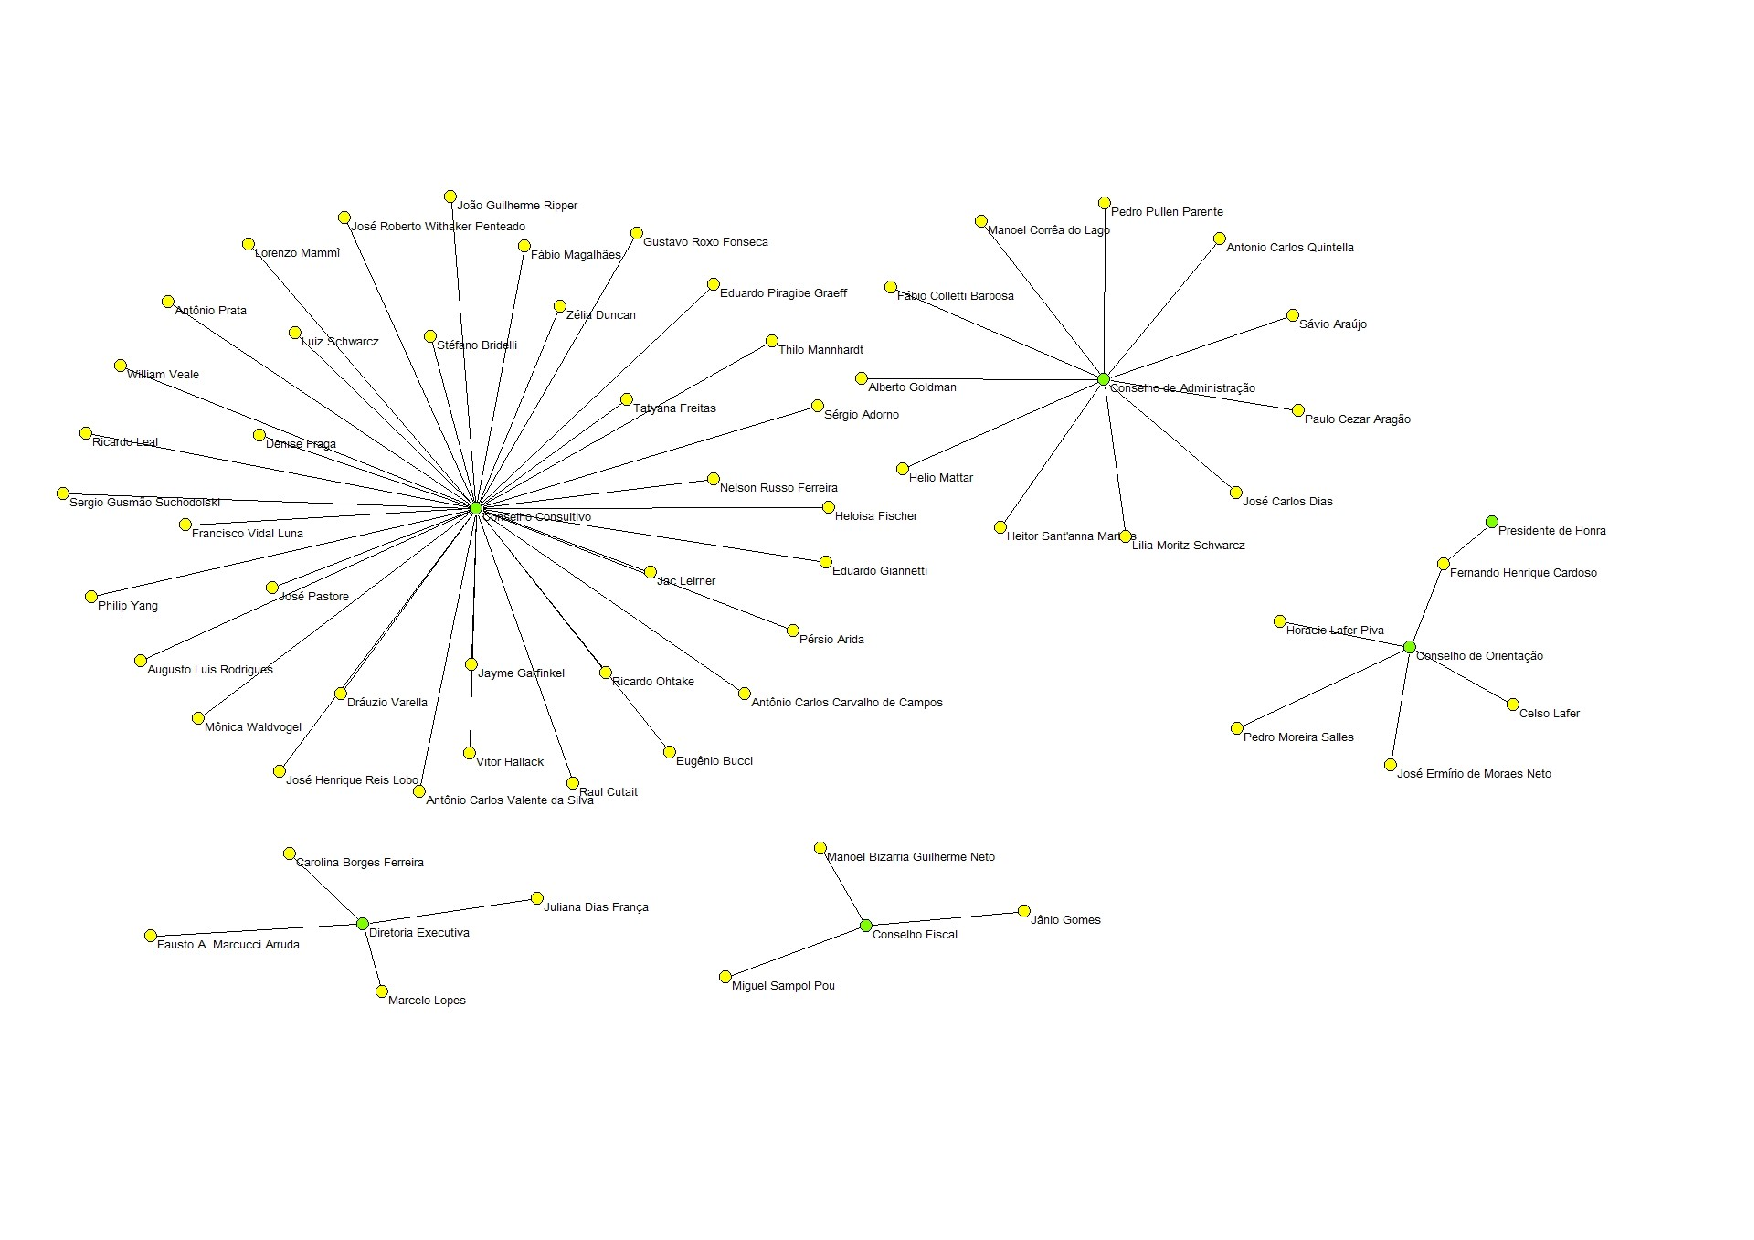
\includegraphics[scale=0.8]{OSESP_conselhos_pajek.pdf}
		\fonte{Site da \citeonline{osesp2016site}. Dados trabalhados pelo autor.}
	\end{sidewaysfigure}
	
	Além dos órgãos supracitados, a Fundação OSESP contém em sua base setores artísticos, pedagógicos e administrativos. São eles a Diretoria Artística, a Orquestra, o Coro, a coordenação artístico-pedagógica do Festival de Inverno de Campos do Jordão (festival de cunho formativo mantido pela Fundação OSESP), departamento jurídico, o Centro de Documentação Musical e Editora Criadores do Brasil, o setor de Atividades Educacionais (responsável pela Academia da Osesp, máster-classes e demais projetos formativos), departamento de marketing, departamento de comunicação, controladoria, contabilidade, departamento financeiro, uma divisão administrativa (composta de gerência, recepção, serviços de copa, serviços terceirizados, recursos humanos, informática, almoxarifado e arquivo), e uma divisão operacional (composta de departamento de produção, departamento técnico, iluminação, som, montagem, departamento de operações, controlador de acesso e indicadores). Essa estrutura está representada na Figura 6.
	
	\begin{sidewaysfigure}
		\centering
		\caption{A estrutura da Fundação OSESP 2}
		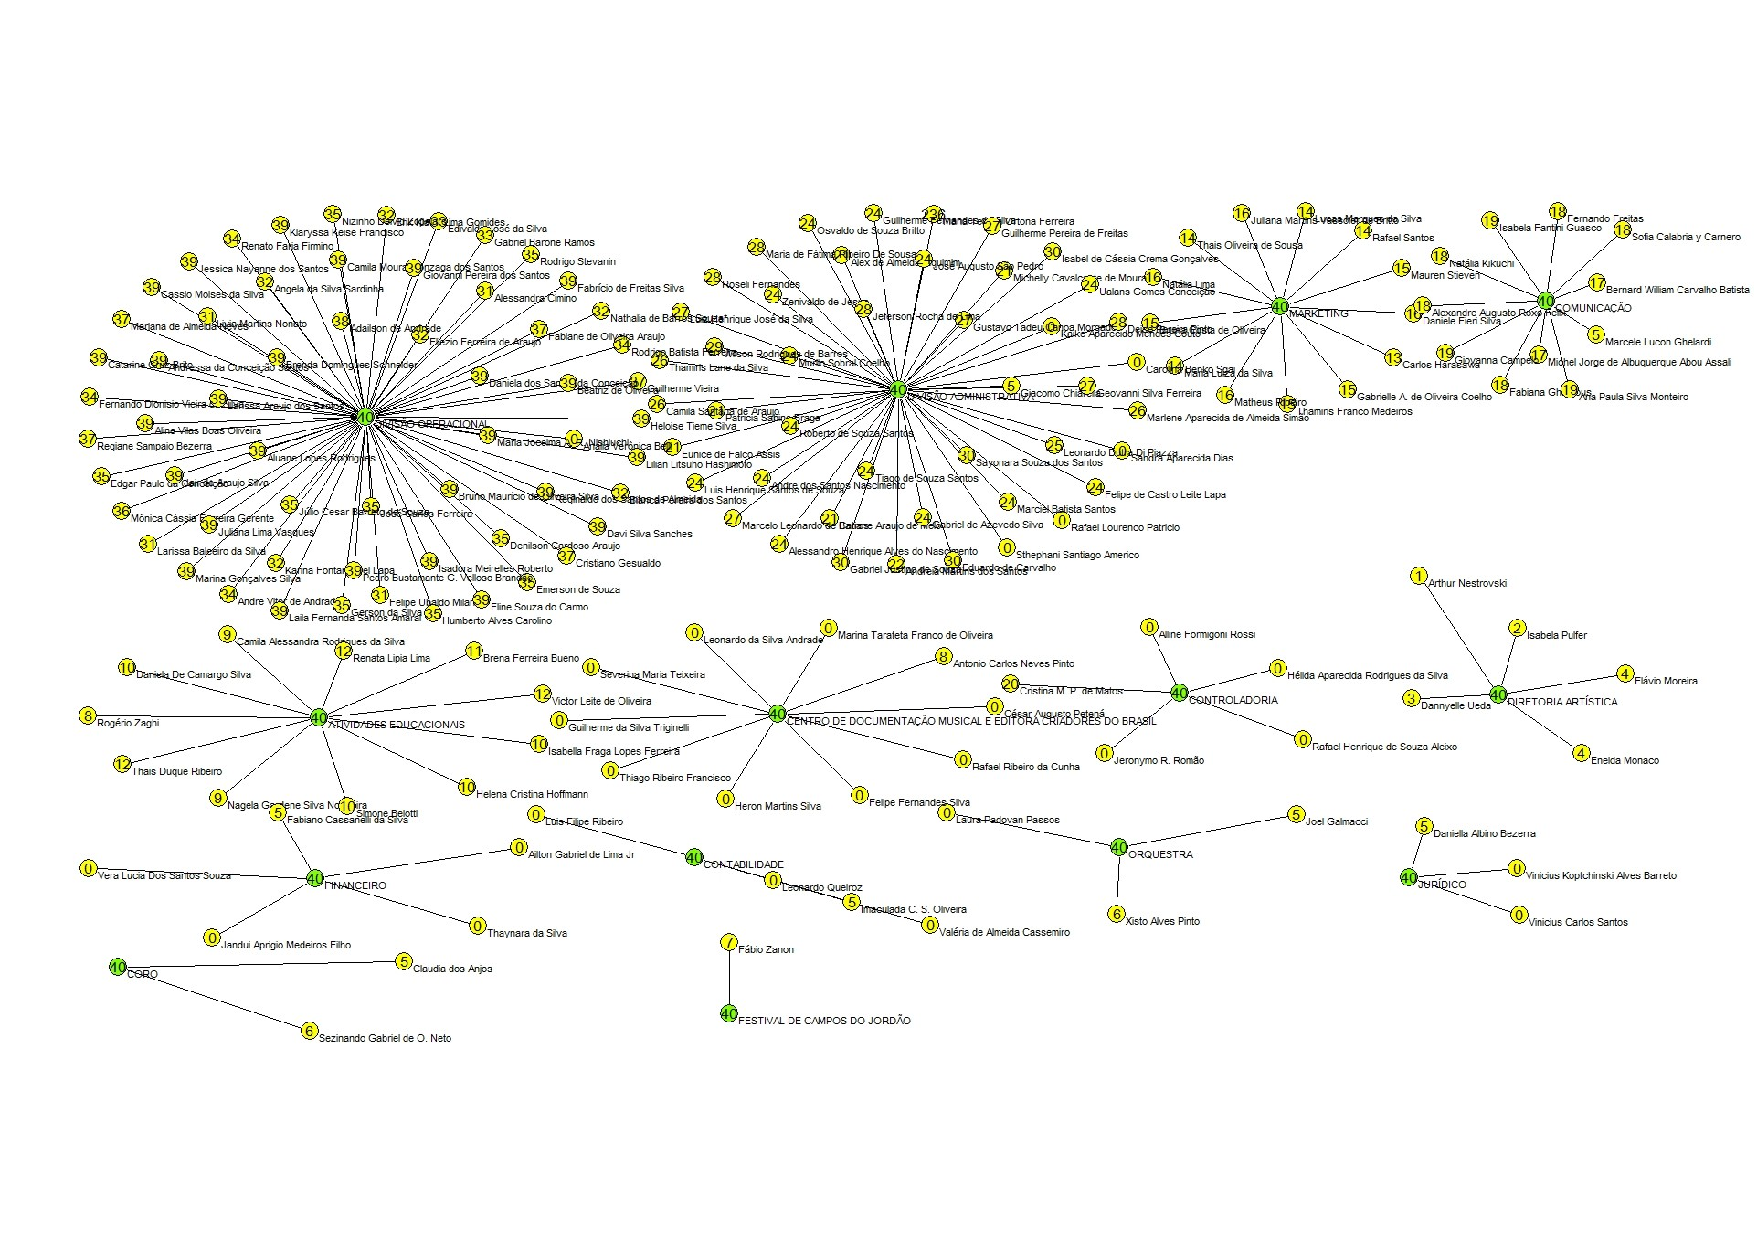
\includegraphics[scale=0.8]{OSESP_setores_pajek.pdf}
		\fonte{Site da \citeonline{osesp2016site}. Dados trabalhados pelo autor.}
	\end{sidewaysfigure}
	
	\subsection{Financiamento}
	
	Os recursos da OSESP provém de fontes diversificadas mas, sobretudo, diretamente do estado de São Paulo conforme o contrato de gestão vigente e, por outro lado, através da iniciativa privada. O Estado de São Paulo investiu, de 2010 a 2015 o montante de R\$251.676.666,67 distribuídos da seguinte forma: R\$7.166.666,67 em 2010, R\$43.400.000,00 em 2011, R\$53.400.000,00 em 2012, R\$55.500.000,00 em 2013, R\$55.650.000,00 em 2014 e R\$36.560.000,00 em 2015\footnote{O volume financeiro previsto para financiamento em 2015 a princípio era de R\$46.816.667,00 o qual foi alterado conforme o 6º termo de aditamento.}.
	
	Em 2014 (dados mais recentes publicados), a OSESP teve um custo total aproximado de R\$100.327.000,00 e uma receita total aproximada de R\$102.339.000,00. A distribuição das receitas por suas fontes estão apresentadas na tabela TAL.
	
	\begin{table}[ht]
		\IBGEtab{
			\centering
			\caption{Distribuição das porcentagens de financiamento da OSESP}
		}
		{\begin{tabular}{rrr}
				\hline
				& Fonte & (\%)\\
				\hline
				1 & Projetos Incentivados & 35 \\
				2 & Locação -- Eventos e Espaços & 18 \\
				3 & Assinatura e Bilheteria & 18 \\
				4 & Receitas Financeiras & 15 \\
				5 & Permutas e Patrocínios & 11 \\
				6 & Venda de Concertos & 3 \\
				7 & Outras Receitas Próprias & 0 \\
				\hline
			\end{tabular}
		}
		{\fonte{Elaboração do autor a partir de \citeonline{osesp2014compromisso}.}}
	\end{table}
	
	Em 2014 a OSESP captou R\$18.190.000,00 junto à iniciativa privada (mediante isenção fiscal) e R\$15.548.000,00 em mídia por meio de permutas. As empresas financiadoras da OSESP estão divididas em 3 categorias conforme o volume de recursos investidos: patrocinadores (valores acima de R\$500.000,00), apoiadores (valores acima de R\%200.000,00)  e outros apoiadores (cf. Figura TAL). O Programa Sua Orquestra, programa de financiamento voltado à captação de recursos junto à pessoas físicas, reuniu 654 associados e arrecadou um montante de R\$980.000,00.
	
	\begin{figure}[!ht]
		\centering
		\caption{Os investidores da OSESP em 2014}
		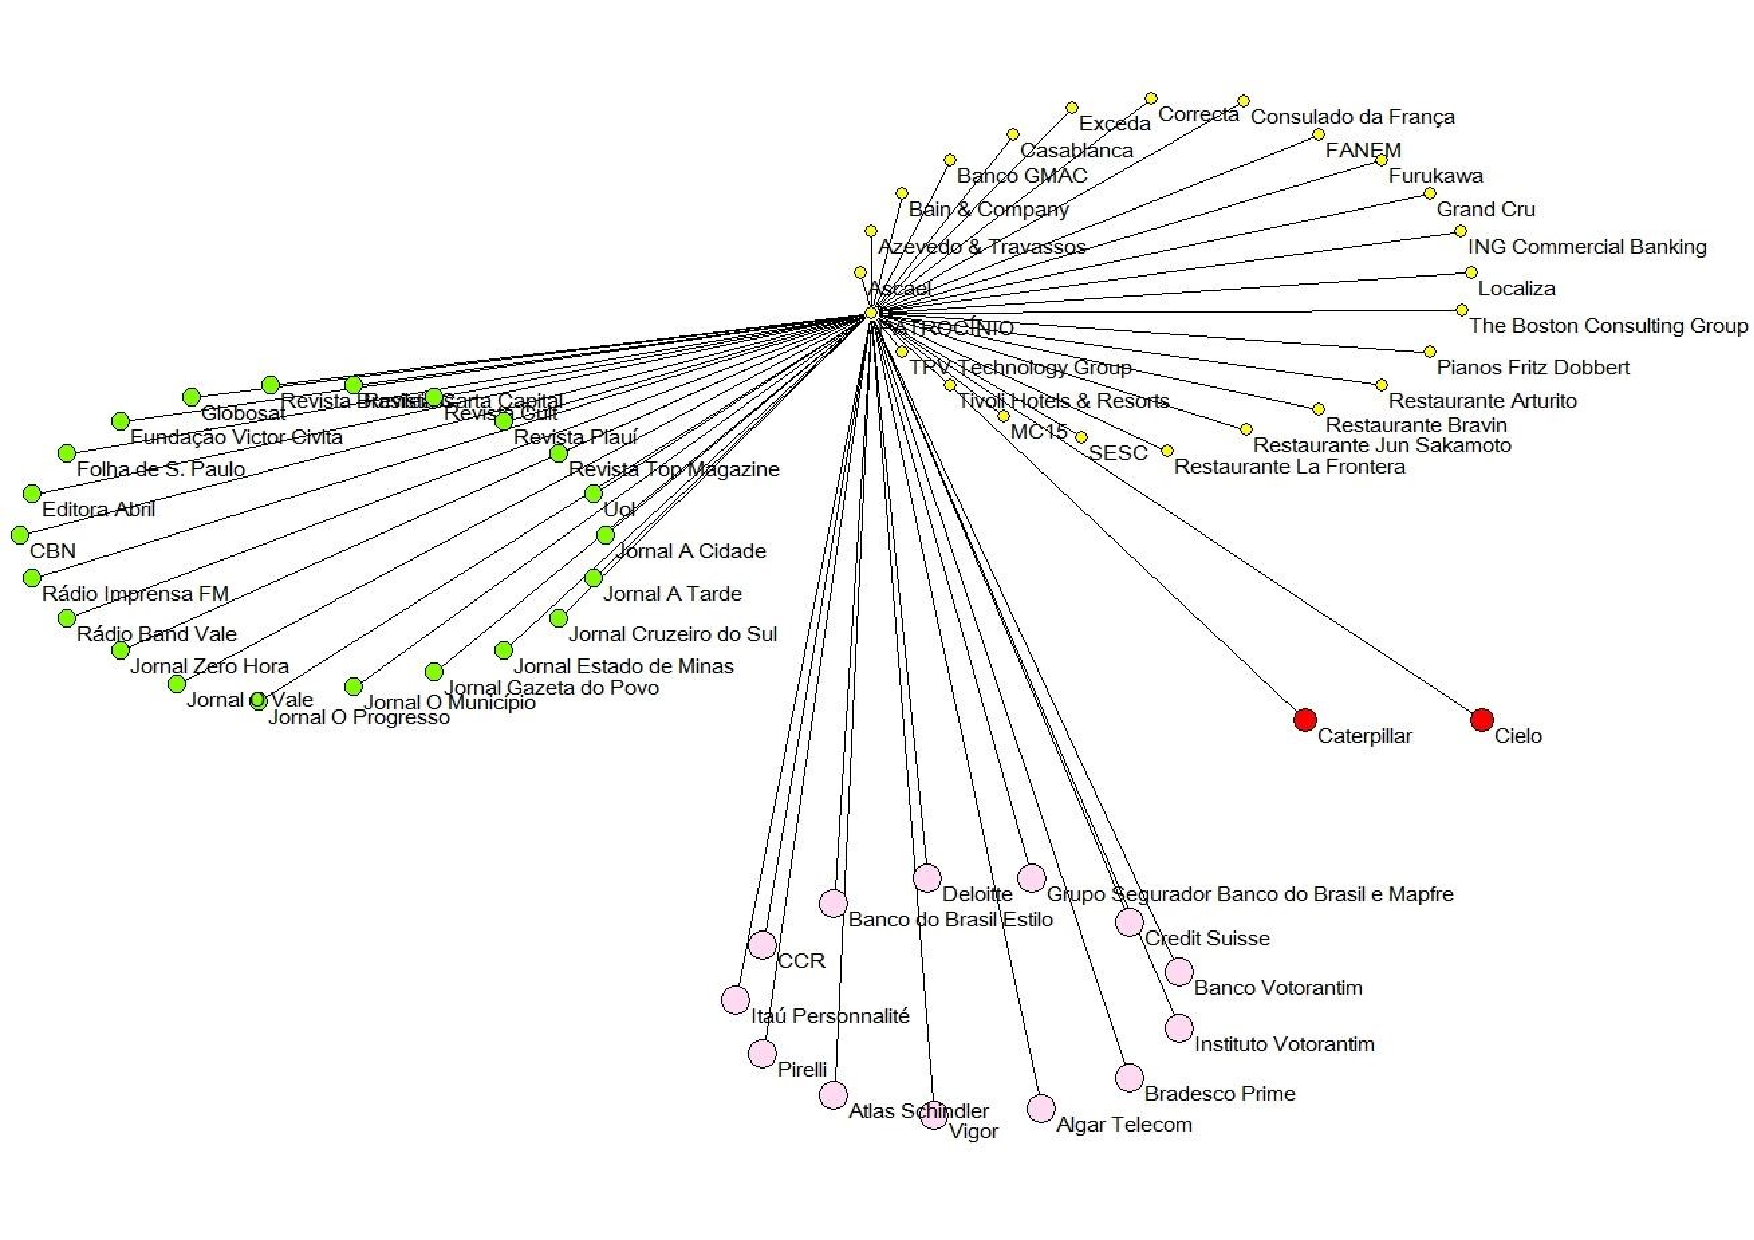
\includegraphics[scale=0.55]{OSESP_patrocinio.pdf}
		\fonte{Elaboração do autor a partir de \citeonline{osesp2014compromisso}.}
		\nota{Vértices rosas são patrocinadores, vermelhos são apoiadores, amarelos são outros apoiadores e verdes são veículos de comunicação parceiros via permuta. Com a exceção do grupo verde, o tamanho dos vértices indica as categorias de volume de investimento.}
	\end{figure}
	
	
	
	
	% Parei aqui!!!!!!!!!!
	%=================================================================
	%=================================================================
	
	
	
	
	
	
	
	
	
	
	
	
	
	\section{A Orquestra Filarmônica de MG}
	
	Criada muito recentemente, em 2008, a Orquestra Filarmônica de MG tem se destacado nos âmbitos nacional e internacional pela qualidade técnica e artística de suas apresentações. (Verificar o histórico da orquestra\ldots)
	
	
	
	A Orquestra Filarmônica de MG pode ser divida em dois grandes setores: a orquestra propriamente dita e sua instituição mantenedora, o Instituto Cultural Filarmônica. A orquestra é composta por cerca de noventa músicos, o maestro e seu assistente, um gerente, um inspetor, um assistente administrativo, quatro arquivistas e seis montadores. Já o Instituto Cultural Filarmônica é formado pela Assembleia de Associados, pelo seu Conselho Administrativo, pela Diretoria Executiva, Equipe Técnica e Equipe Administrativa.
	
	A Diretoria Executiva do Instituto é formada pelo Diretor Presidente, pelo Diretor Administrativo-financeiro, pela Diretora de Comunicação, pela Diretora de MKT e Projetos, pelo Diretor de Operações e pelo Diretor de Produção Musical. A equipe técnica é formada pelo Gerente de Comunicação, Gerente de Produção Musical, Assessor de Programação Musical, Produtores, Analistas de Comunicação, Analista de MKT de Relacionamento, Analistas de MKT e Projetos, Assistente de MKT de Relacionamento, Assistente de Procução e quatro profissionais alocados na Sala Minas Gerais (Gerente de Infraestrutura, Gerente de Operações, Assistente Operacional e Técnico de Iluminação e Áudio). A equipe administrativa é formada pelo Gerente Administrativo-financeiro, Gerente de Recursos Humanos, Analistas Administrativos, Analista Contábil, Secretária Executiva, Assistente Administrativa, Assistente de Recursos Humanos, Recepcionista, Auxiliar Administrativo, Auxiliares de Serviços Gerais, Mensageiros e um menor aprendiz (FIG. 2).
	
	\begin{figure}[h]
		\centering
		\caption{Organograma da Orquestra Filarmônica de MG e do Instituto Cultural Filarmônica}
		%\includegraphics[keyvals]{imagefile}
		\fonte{Elaboração do autor a partir de dados disponíveis online}
	\end{figure}
	
	Em seu funcionamento, ambos os setores se envolvem em relações comerciais ou artísticas com outros atores. No caso da orquestra, é comum a visita de solistas e maestros convidados. No caso do Instituto, uma rede de fornecedores nos mostra o âmbito dos recursos necessários à mobilização. Dentre os fornecedores do Instituto há assessoria contábil, assessoria jurídica, assessoria de imprensa, assessoria em TI, \textit{clipping}, criação e finalização de som, fotógrafos, gestão de projetos culturais, gráfica rápida, impressão digital, produção audiovisual, produção gráfica, sistema de assinaturas e compra de ingressos, serviços de segurança eletrônica, sistema de gestão e a redação de notas para os programas dos concertos (FIG. 3). 
	
	\begin{sidewaysfigure}[!ht]
		\centering
		\caption{O Instituto Cultural Filarmônica e os recursos mobilizados}
		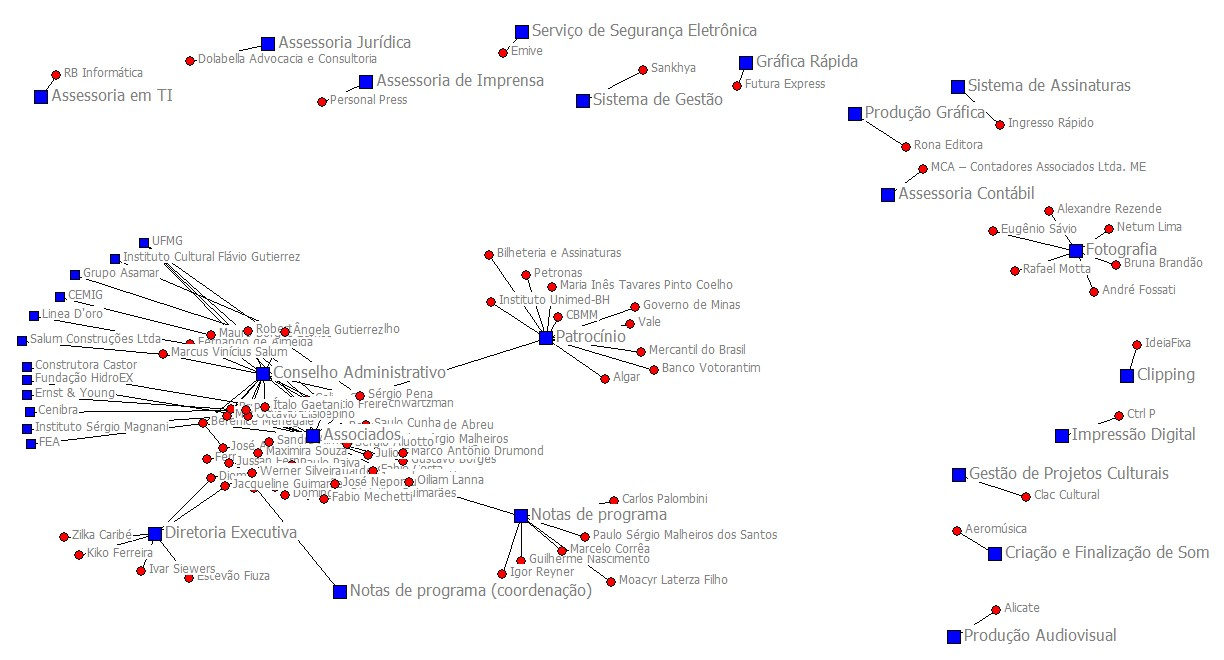
\includegraphics[scale=0.5]{filarmonica_rede2mode.eps}
		\fonte{Elaboração do autor com dados disponíveis online \cite{filarmonica2015site}.}
		\label{fil2mode}
	\end{sidewaysfigure}
	
	Apenas observando o grafo da Figura 3 é possível perceber a complexidade da teia de recursos que o Instituto mobiliza no decurso de suas atividades cotidianas. Além dos serviços de caráter administrativo como assessorias contábil, jurídica, de TI e outros serviços comuns no campo da cultura como gráfica rápida, fotografia e assessoria de imprensa, é curioso notar alguns serviços que parecem peculiares (embora não exclusivos) ao universo da orquestra. A redação das notas de programa é feita por professores de universidades públicas e pesquisadores vinculados a programas de pós-graduação no exterior. Essas notas de programa geralmente funcionam como um guia ao ouvinte e são inseridas no ``Fortíssimo'', uma publicação mensal da orquestra contendo ainda as biografias dos maestros e solistas convidados e notícias da orquestra. Mais do que um simples programa de concertos, o ``Fortíssimo'' é uma publicação indexada em sistemas nacionais e internacionais de catalogação. As notas de concerto geralmente informam o expectador sobre alguns pontos importantes da biografia do compositor, algumas questões estéticas e estilísticas envolvendo a obra programada para execução além de algumas sugestões de escuta da obra e leitura relacionada. A publicação é distribuída gratuitamente e, ao fim dos concertos, os ouvintes tem a oportunidade de retorná-la, caso não queiram guardá-la.
	
	O Instituto também mantém uma relação comercial com uma empresa especializada em gestão de projetos culturais. Isso faz sentido se sabemos que uma boa fatia dos recursos captados pela orquestra o são mediante projetos de isenção fiscal. Exploraremos em maiores detalhes esse financiamento oportunamente. \textit{Por ora, faz-se necessário investigar com maior profundidade de que modo o Instituto compartilha sua gestão com esse fornecedor.} (DESENVOLVER)
	
	\subsection{Recursos Financeiros}
	
	A Orquestra Filarmônica conta em 2015 com um financiamento de R\$22.348.993,00 proveniente de fontes diversificadas. A instituição recebe fundos direto do Governo de Minas, seu principal financiador, de empresas investidoras através de leis de incentivo à cultura e do público pagante (FIG.4).
	
	\begin{figure}[t]
		\begin{center}
			
			\caption{Os financiadores da Filarmônica}
			\begin{center}
				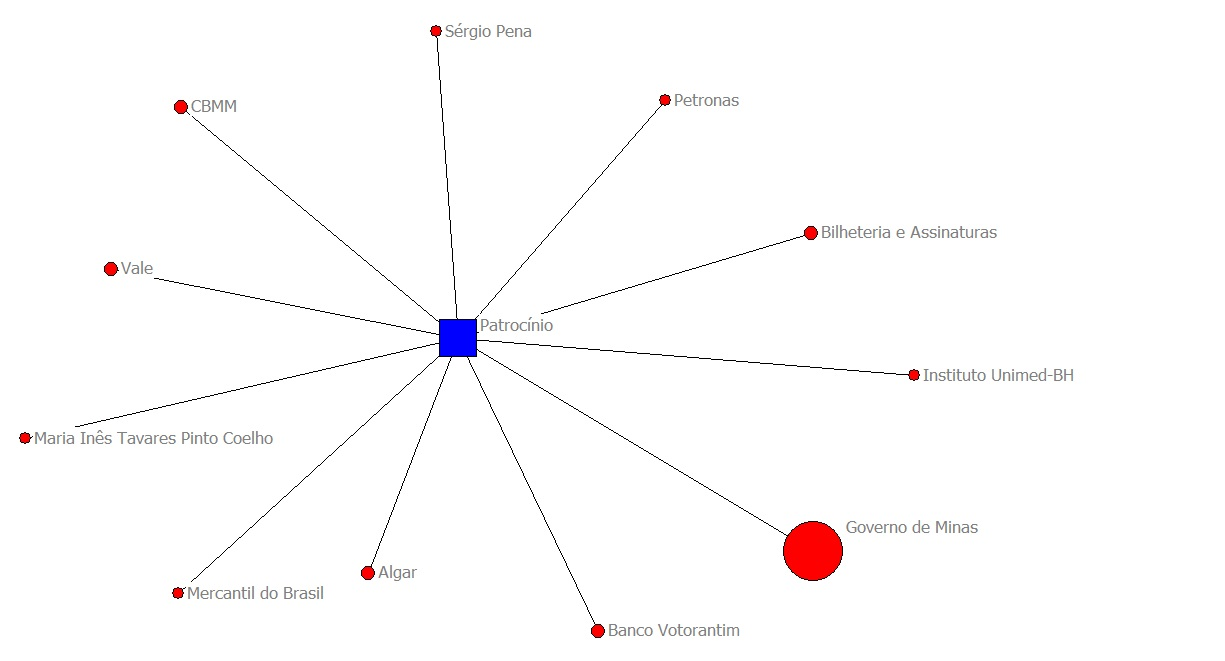
\includegraphics[scale=0.6]{filarmonica_patrocinadores.eps}
			\end{center}
			\fonte{Elaboração do autor a partir de \citeonline[p. 13]{minas2015} e \citeonline[p. 23-4]{filarmonica2015gerencial}. Os tamanhos dos vértices no grafo indicam o volume de capital investido na instituição.}
		\end{center}
	\end{figure}
	
	Seu maior financiador, o Governo de Minas é responsável por 81,69\% de seu financiamento total. 
	
	% latex table generated in R 3.2.1 by xtable 1.7-4 package
	% Thu Oct 15 01:17:07 2015
	\begin{table}[ht]
		\IBGEtab{
			\centering
			\caption{Fontes de financiamento da Filarmônica em 2015}
		}
		{\begin{tabular}{rrrrc}
				\hline
				& Fontes & Montantes (R\$) & (\%) & \% acumulada \\ 
				\hline
				1 & Algar & 595.400,00 & 2.66 & 2.66 \\ 
				2 & Banco Votorantim & 900.000,00 & 4.03 & 6.69 \\ 
				3 & Bilheteria e Assinaturas & 736.312,82 & 3.29 & 9.99 \\ 
				4 & CBMM & 500.000,00 & 2.24 & 12.22 \\ 
				5 & Governo de Minas & 18.257.024,50 & 81.69 & 93.91 \\ 
				6 & Instituto Unimed-BH & 299.955,68 & 1.34 & 95.26 \\ 
				7 & Maria Inês Tavares Pinto & 300,00 & 0.001 & 95.26 \\ 
				8 & Mercantil do Brasil & 207.000,00 & 0.93 & 96.18 \\ 
				9 & Petronas & 150.000,00 & 0.67 & 96.85 \\ 
				10 & Sérgio Pena & 3.000,00 & 0.01 & 96.87 \\ 
				11 & Vale & 700.000,00 & 3.13 & 100.00 \\ 
				\hline
				& TOTAL & 22.348.993,00 &  & \\
				\hline 
			\end{tabular}
		}
		{\fonte{Elaboração do autor a partir de \citeonline[p. 13]{minas2015} e \citeonline[p. 23-4]{filarmonica2015gerencial}.}
		}
	\end{table}
	
	Fica claro o papel decisivo do Estado como mantenedor da Orquestra Filarmônica de MG. Sem mais de 80\% de seu orçamento anual imaginamos que seria bastante difícil para os dirigentes manterem a cota de concertos e os convites a maestros e solistas convidados. 3.3\% do orçamento provém do pagamento de ingressos e assinaturas. Em termos absolutos, o valor representa uma quantia vultuosa se comparado ao campo cultural de um modo geral. Entretanto, representa uma pequena fatia no financiamento da orquestra.
	
	O restante do financiamento da instituição vem de empresas privadas por meio do mecanismo de incentivo fiscal das leis de incentivo à cultural federal e estadual. Na modalidade de incentivo fiscal, a lei federal (Rouanet) concede às empresas financiadoras de cultura no Brasil uma porcentagem de desconto no Imposto de Renda (IR). A lei estadual de Minas Gerais concede desconto no Imposto sobre Circulação de Mercadorias e Serviços (ICMS). O volume de financiamento adquirido via lei Rouanet corresponde a 12,35\% do total enquanto aquele adquirido via lei estadual, 2,66\% (apenas a empresa Algar patrocina por esse meio). Curioso notar que, apesar de as empresas constarem como financiadoras da orquestra, de fato o dinheiro investido provem de isenção fiscal, portanto, dinheiro público. Mesmo os investimentos feitos por pessoas físicas (dois casos) também acontecem mediante isenção fiscal. O Estado aparece aqui como um grande centralizador do financiamento da orquestra. Nessa afirmação não nenhum louvor ou crítica. Pergunto-me se, caso o Estado não se colocasse com presença tão forte, o setor privado investiria o montante que vimos.
	
	\textit{Aqui é preciso investigar como o Instituto cria os laços com o setor privado.} (DESENVOLVER) 
	
	%\subsection{O Estado e as leis de incentivo à cultura}
	
	%\textit{Investigar aqui como funciona o papel do Estado no financiamento da instituição de um modo mais holístico}. (DESENVOLVER)
	
	\section{A Orquestra Sinfônica de Minas Gerais}
	
	A OSMG, diferente dos outros dois casos analisados supra, é uma orquestra pública formada por funcionários estatutários.
	
	Segue o organograma da instituição mantenedora da OSMG, a Fundação Clóvis Salgado.
	
	\begin{figure}[ht]
		\centering
		\caption{Fundação Clóvis Salgado -- Organograma}
		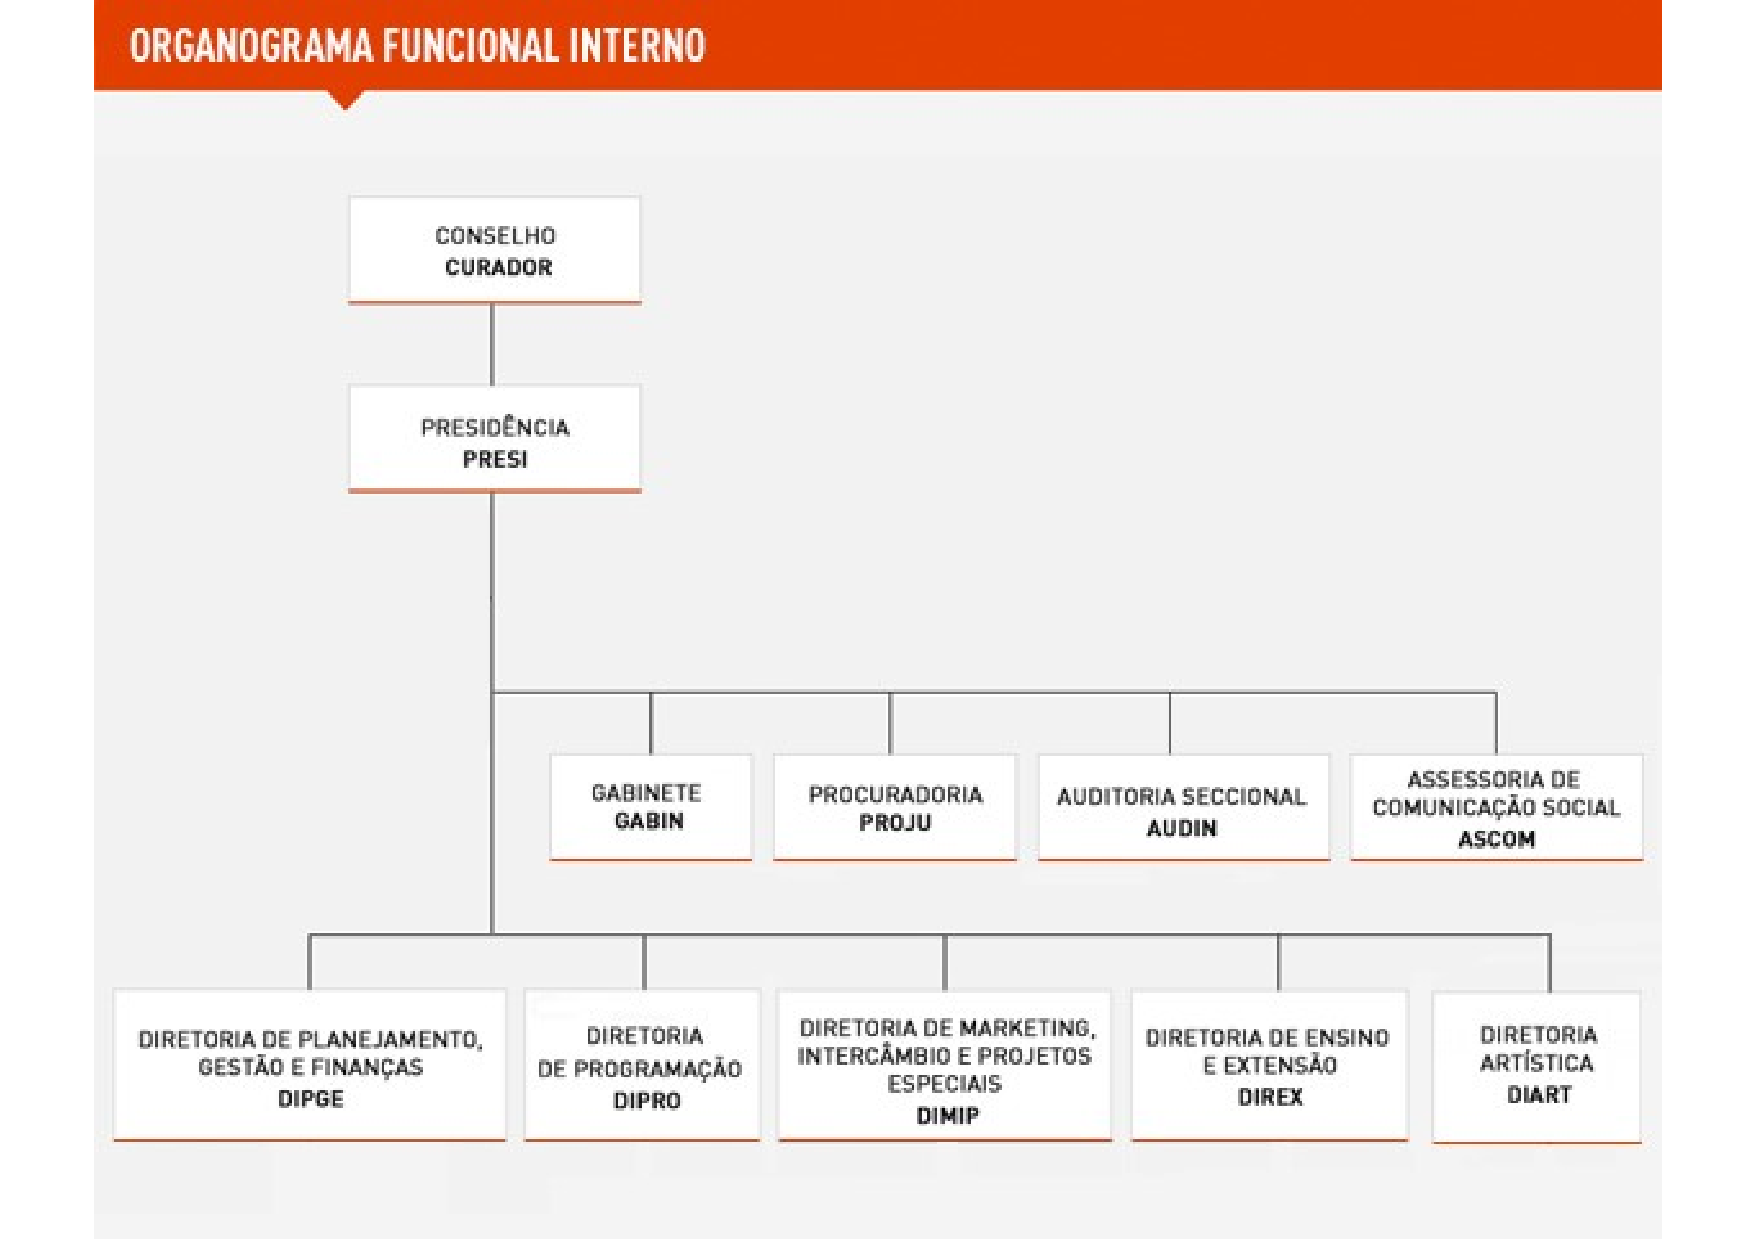
\includegraphics[scale=0.57]{organogramaFCSred.pdf}
		\fonte{Site da \citeonline[http://fcs.mg.gov.br/institucional/organograma]{fcs2016site}.}
		\label{fcsorg}
	\end{figure}
	
	\begin{sidewaysfigure}[ht]
		\centering
		\caption{Fundação Clóvis Salgado -- Diretorias}
		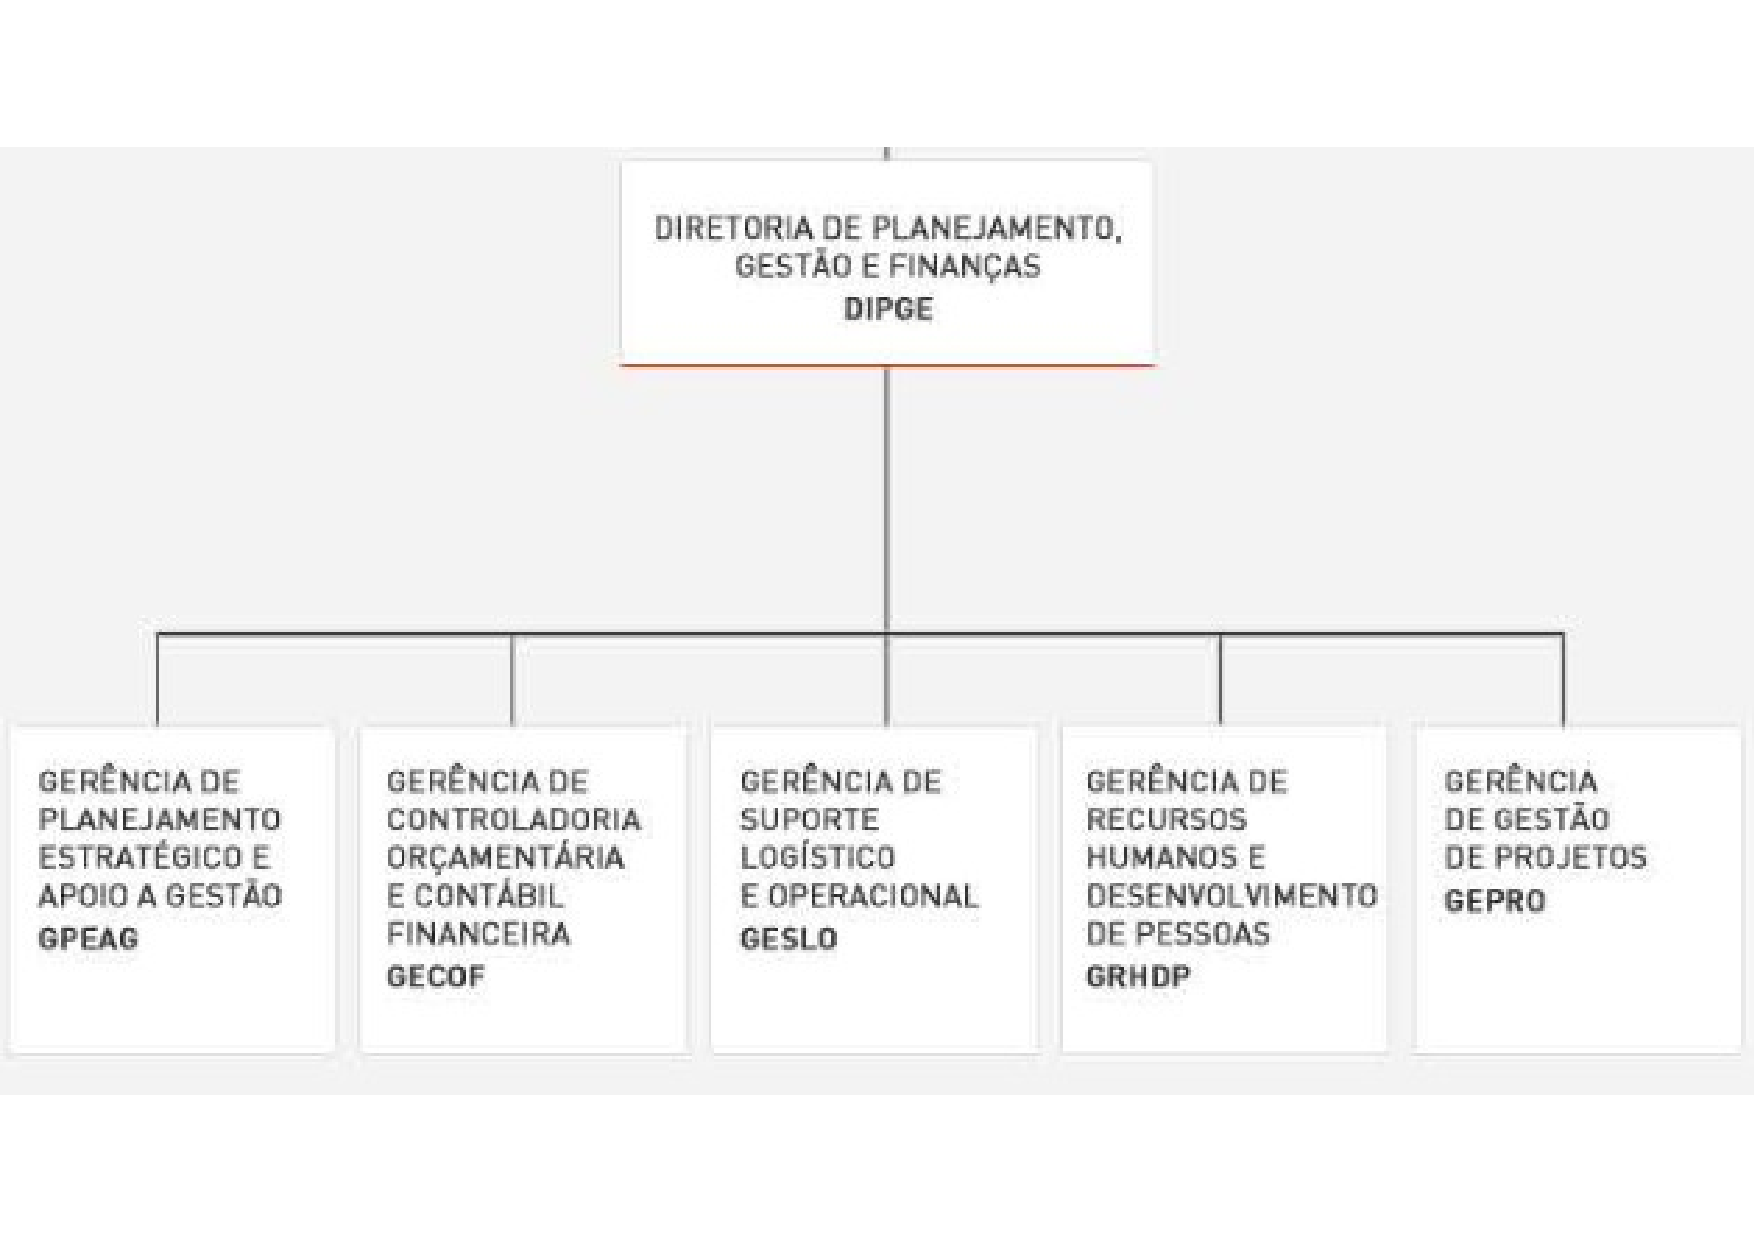
\includegraphics[scale=0.35]{dirplanejamento.pdf}
		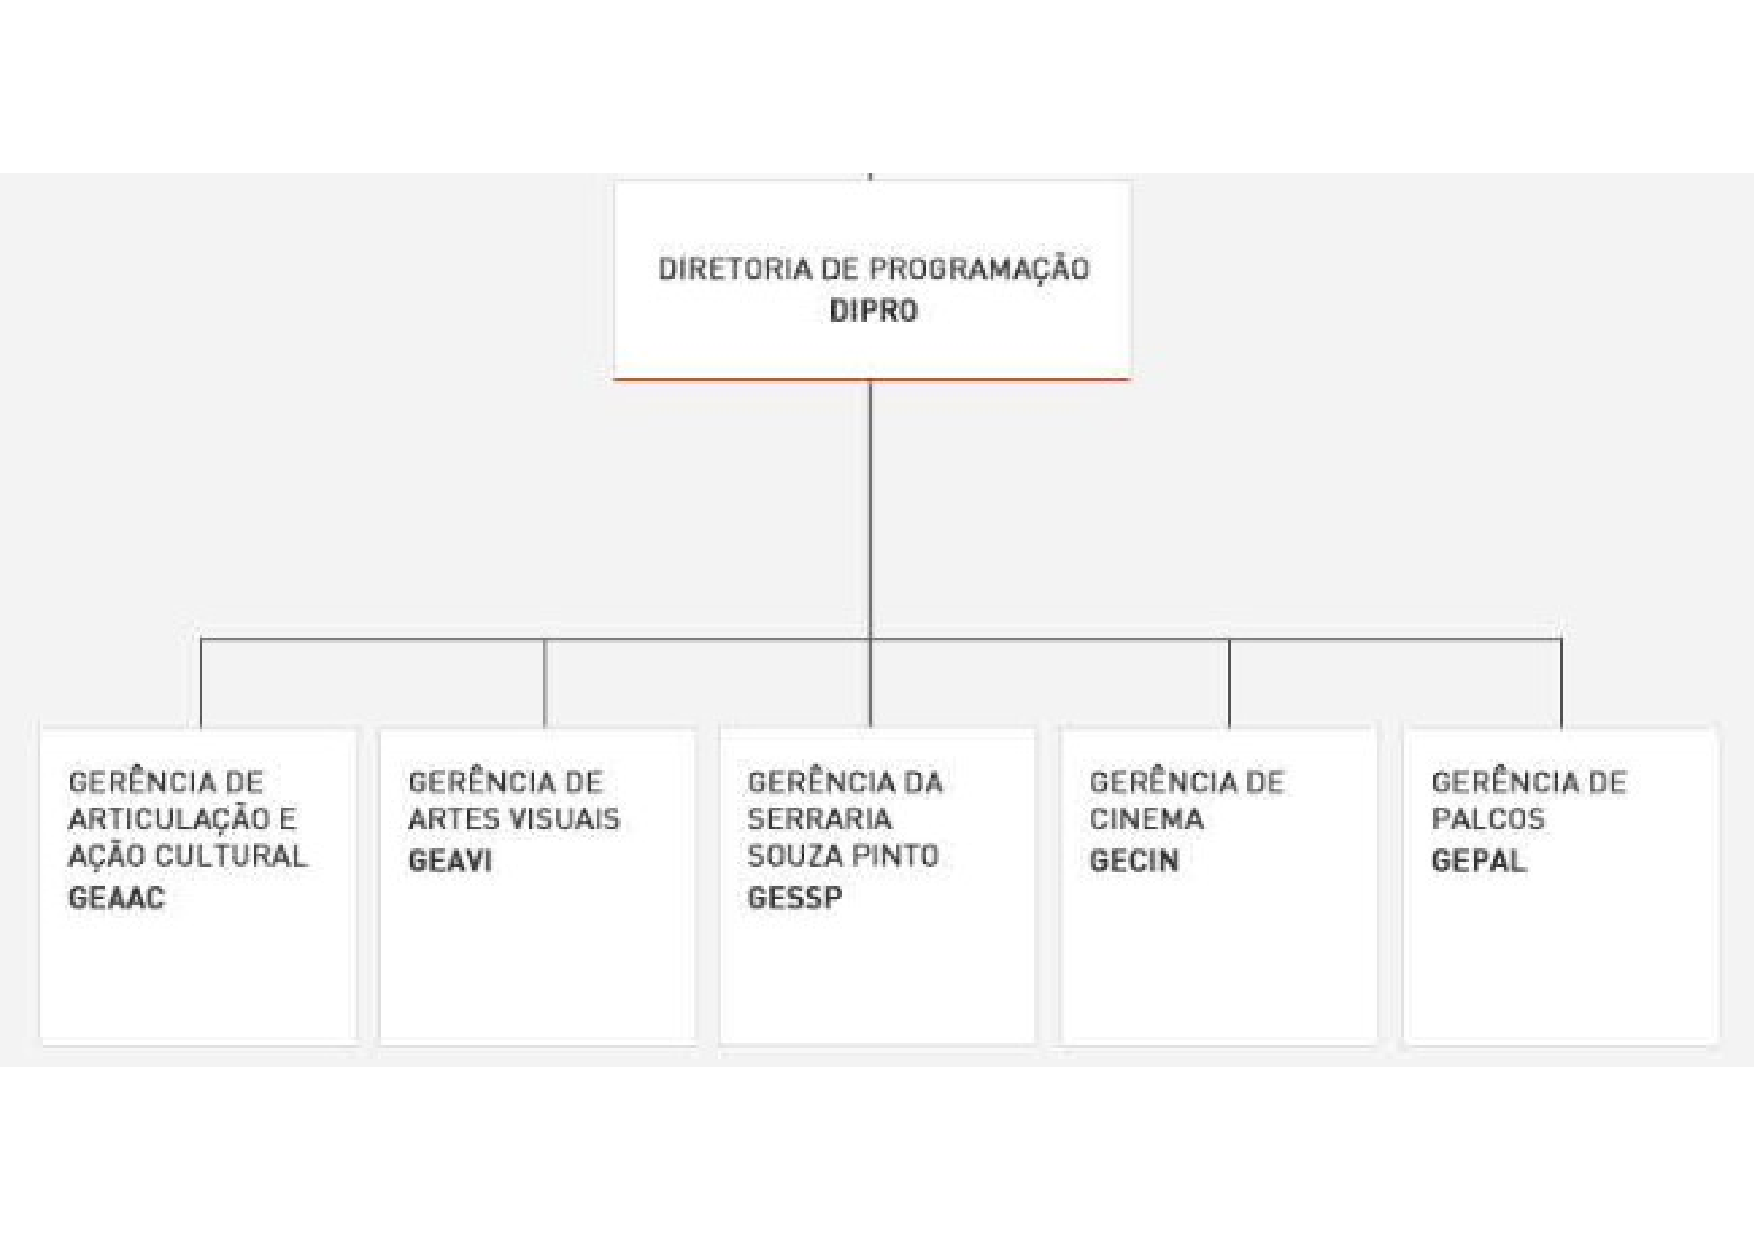
\includegraphics[scale=0.35]{dirprogramacao.pdf}
		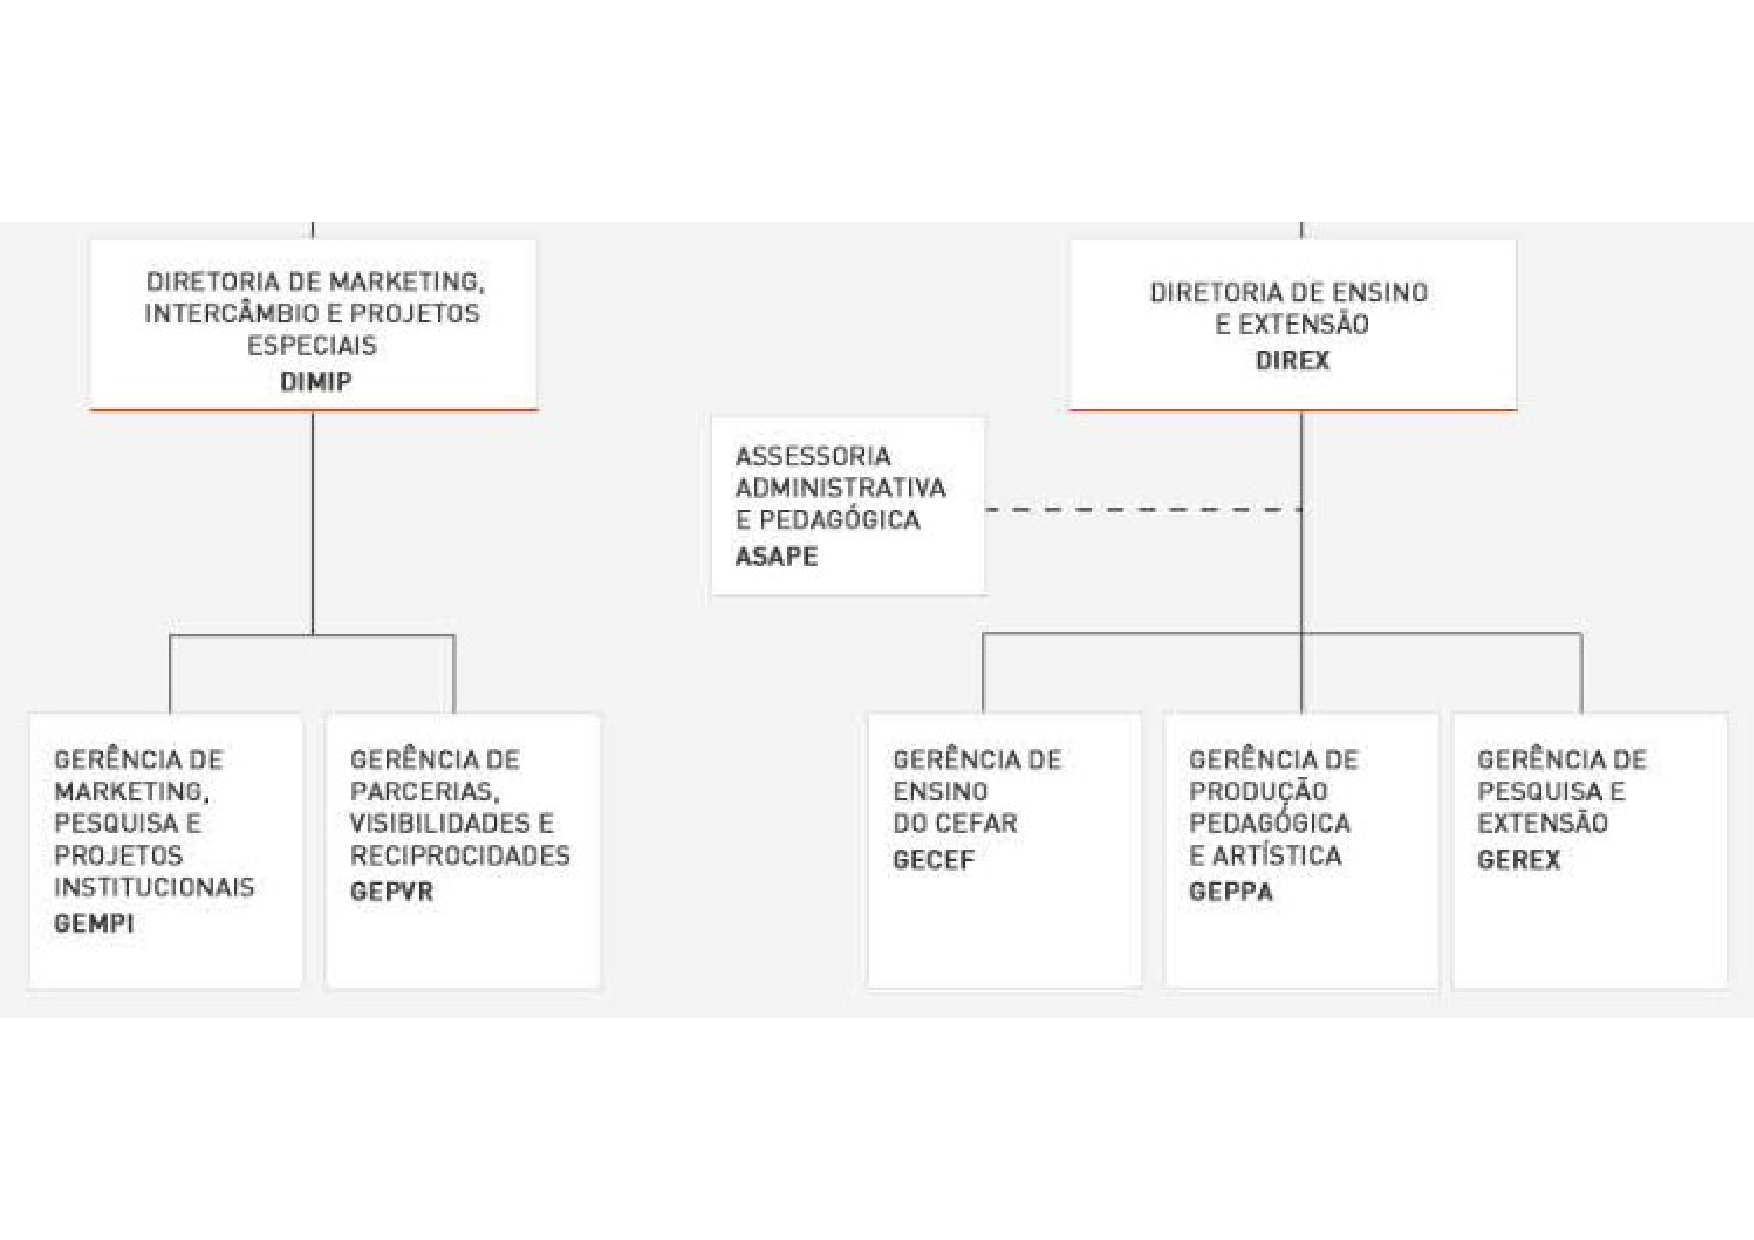
\includegraphics[scale=0.35]{dirmarketingensino.pdf}
		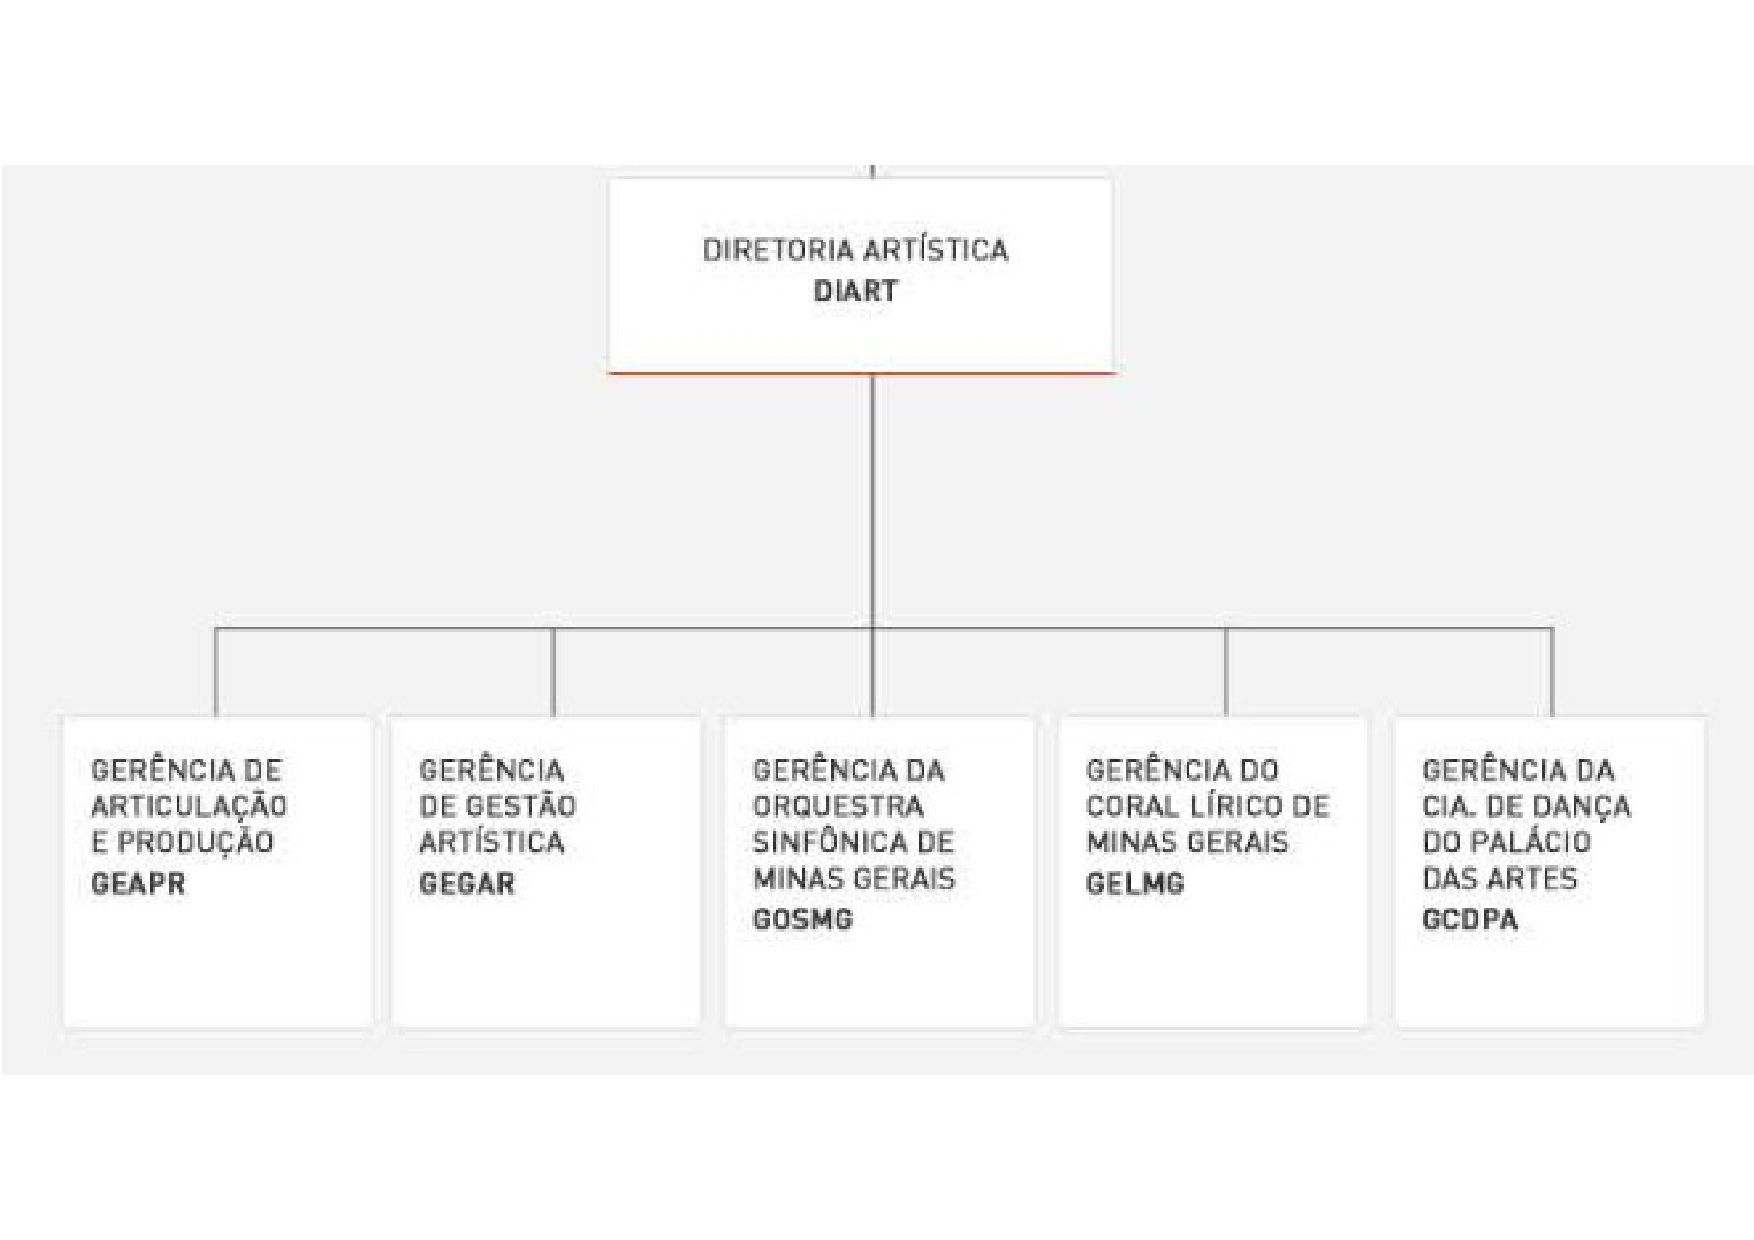
\includegraphics[scale=0.35]{dirartistica.pdf}
		\fonte{Site da \citeonline[http://fcs.mg.gov.br/institucional/organograma]{fcs2016site}.}
		\label{fcsorgdir}
	\end{sidewaysfigure}
	
	
	
	\chapter{A articulação do mercado de produção de música de concerto}
	
	A ideia aqui é explicitar, de acordo com a teoria neoestrutural dos mercados traçada no capítulo 1 a partir de \citeonline{white2002markets}, \citeonline{lazega2009theorie} e \citeonline{fligstein2002architecture}, como se articula o mercado das orquestras nas cidades escolhidas\ldots
	
	
	\chapter{A Construção Social da Qualidade}
	
	A qualidade atribuída a um produto cultural, como vimos, é um fator crucial para a articulação do mercado. De acordo com \citeonline{white2002markets}, a qualidade e a identidade dos atores num mercado não emanam um do outro mas se produzem mutuamente ao longo de um set de interações entre eles. A qualidade é concebida aqui não como um atributo evidente mas como uma sutil construção social. Esta visão servirá de base para as investigações aqui empreendidas. Tratemos de melhor delineá-la.
	
	Para \citeonline{white2002markets}, o mecanismo pelo qual funcionam os mercados de produção está ancorado sobre bases que mergem da interação entre julgamentos de todos os atores da rede, produtores e consumidores. O autor continua
	
	\begin{citacao}
		No mundo real dos negócios, questões de qualidade são juntamente imputadas a propriedades que foram amontoadas juntas como um ``produto'', mesmo que essas propriedades possam parecer ao observador variadas e, de certo modo, arbitrárias. Esse amontoado é percebido com respeito ao mercado do produto como um todo, a fonte para a qual todos se voltam por esse amontoado. Produtores procuram e percebem diferenciação na apreciação -- o índice de qualidade -- para suas versões particulares daquele produto do mercado. E, de fato, normalmente haverá um conjunto de variantes por tamanho, cor, etc. do carregamento daquela firma havendo, desse modo, amontoamento no nível da firma também\footnote{In actual business life, quality meanings become jointly imputed to properties that have gotten bundled together as a ``product'', even though these properties may seem to an observer various and somewhat arbitrary. This bundle is perceived with respect to the product market as a whole, the source to which everyone turns for that bundle. Particular producers seek and realize differentiation in appreciation --the quality index -- fot their particular versions of that market product. And indeed, there often will be a cluster of variants by size, color, and so forth of that firm's product shipments, so that there is bundling at the firm level also.}. \cite[p. 10, tradução do autor]{white2002markets}
	\end{citacao}
	
	Se transportamos a declaração supracitada de White para o mercado da produção de música erudita é fácil identificar que as proposições permanecem verdadeiras. A qualidade de uma orquestra é percebida num amontoado de outras propriedades atribuídas àquela orquestra (prestígio, orçamento, nacionalidade dos músicos\footnote{No caso brasileiro, a nacionalidade dos músicos componentes de uma orquestra parece ser um fator importante na atribuição de qualidade à orquestra. O público tende a superestimar orquestras que tenham músicos que nasceram ou estudaram em países com tradição de música erudita como Alemanha, França, Rússia, Itália, etc.}, conforto e tamanho da sala de concertos, etc.) e os produtos oferecidos, i.e., o repertório escolhido para performance, assume alguma variação de interpretação por orquestra\footnote{Para um estudo aprofundado sobre como as performances orquestrais variam com cada maestro e cada orquestra, consultar \citeonline{crepalde2015maestro}.}.
	
	\citeonline[p. 10]{white2002markets} salienta outro ponto importante para nós no que tange à qualidade: ``Interação de escolhas pressupõe um estabelecimento a priori de comparabilidade''
	\footnote{Interaction of choices presupposes prior establishment of comparability.}. A forma mais simples de comparabilidade consiste de uma escala linear de qualidade entre as empresas. A reputação distribuída de uma maneira desigual é, para White, a moeda da disciplina para os mercados de produção. Por esse motivo, não é possível que os mercados de produção contenham mais do que algumas empresas por causa das limitações cognitivas. De fato, ``linhas de negócios reconhecíveis são constituídas por um número modesto de firmas, tipicamente menos que vinte''\footnote{Recognizable lines of business are constituted in and by some modest number of firms, tipically fewer thant twenty.}, o que sabemos através do legado da economia dos custos de transação \apud{williamson1975markets}{white2002markets}.
	
	A qualidade, entretanto, não é algo dado mas uma construção social que emerge da interação de atores interligados em domínios em rede (\textit{netdoms}). 
	
	
	
	
	
	\begin{comment}
	\section{Dados e métodos}
	
	Investigamos aqui a emergência da qualidade num domínio em rede através de um modelo de difusão social (\textit{network diffusion model}). Esse modelo é realizado através de simulações computacionais onde o pesquisador simula interações entre os agentes dados alguns pressupostos. Esse tipo de método é utilizado numa grande variedade de campos do conhecimento, de difusão de inovações tecnológicas a contágio e infecções.
	
	Segundo \citeonline[p. 98]{valente2005network}, ``a teoria da difusão de inovações tenta explicar como novas ideias e práticas se espalham dentro e entre comunidades''\footnote{Diffusion of innovations theory attempts to explain how new ideas and practices spread within and between communities.}. Esta teoria está ancorada na antropologia, na economia, na geografia, na sociologia e em várias outras áreas das humanidades aplicadas. ``A premissa, confirmada por pesquisa empírica, é que novas ideias e práticas se espalham através de contatos interpessoais sobretudo por meio da comunicação interpessoal''\footnote{The premise, confirmed by empirical research, is that new ideas and practices spread through interpersonal contacts largely consisting of interpersonal communication.} \cite{ryan1943diffusion,beal1955farm,katz1963traditions,valente1995network,valente1995origins,rogers2003diffusion}.
	
	Nas simulações realizadas, programamos 3 cenários, do mais ``abstrato'' ao mais ``empírico''. A primeira escolha pertinente está relacionada com a topologia\footnote{Chamamos de topologia a rede que será utilizada nas simulações. Todas as interações simuladas acontecerão dentro das limitações dessa rede.} simulada. Simulamos uma rede tipo ``pequeno mundo'' e uma rede livre de escala como topologias.
	
	No primeiro cenário, cada indivíduo pode executar três ações de acordo com as probabilidades atribuídas: (1) ir a um concerto, (2) ler as críticas do concerto e (3) conversar com os amigos sobre o concerto. Cada uma dessas ações recebe uma probabilidade atribuída arbitrariamente. 
	
	No caso da primeira ação, em cada rodada, é gerado um número aleatório entre 0 e 1. Se este número for menor do que a probabilidade fixada de ir a um concerto, segue o código onde um novo número aleatório\footnote{Este número aleatório é gerado dentro de uma distribuição normal com média 3 e desvio padrão 1.} é gerado. Ao agente é atribuído uma classificação final que consiste da média aritmética do valor aleatório e de sua classificação prévia. As classificações prévias foram geradas aleatoriamente numa distribuição normal com média 3 e desvio padrão 1. Os valores iniciais foram arredondados para número inteiros de 1 a 5.
	
	No caso das críticas dos concertos, dois valores aleatórios são gerados: uma probabilidade de ``ler'' as críticas do concerto e uma probabilidade de adoção das críticas. No primeiro momento, se o número aleatório gerado for menor do que a probabilidade de ler as críticas, seguimos com o código. No segundo momento, se o valor aleatório for menor do que a probabilidade de adoção, a clasificação prévia do agente é substituída pelo valor da crítica. Do contrário, a classificação final do agente é obtida através da média aritmética do valor da crítica e de sua classificação prévia.
	
	No caso das interações, em cada rodada o agente ``conversa'' com seus amigos, ou seja, aqueles outros agentes com os quais tem um laço. É gerado um número aletório que, se menor do que a probabilidade de concordar fixada, transforma a classificação final do agente em uma média das classificações prévias dos dois agentes. Caso contrário, ambas as classificações ficam como estão, sem alterações. Este processo será apresentado de forma resumida, abaixo, como foram programadas no formato de pseudo-código. O código originalmente usado em linguagem \textit{Python} pode ser consultado no repositório GitHub\footnote{\url{http://github.com/neylsoncrepalde/diffusion_models}}.
	
	
	
	
	\begin{algorithm}
		\caption{Simulações}\label{sim-geral}
		\begin{algorithmic}[1]
			\Function{Simulação}{Prob\_ler\_crítica, Prob\_adotar\_crítica, Prob\_concordar, Prob\_ir\_ao\_concerto, Crítica}
			
			\While{True}
			\If{Rodada $< 25$} \Comment{Antes da metade}
			\State Críticas $\gets x$
			\Else			   \Comment{Depois da metade}
			\State Críticas $\gets x+1$ ou $x-1$
			\EndIf
			\State \Call{Ir ao concerto}{}
			\State \Call{Ler críticas}{}
			\State \Call{Conversar com amigos}{}
			\EndWhile
			\EndFunction
			
			
			\Function{Ir ao concerto()}{}
			\State Class. do concerto $\gets N\acute{u}mero\ aleat\acute{o}rio \sim \mathcal{N}(3,1)$
			\If{ $\{aleat\acute{o}rio \ | \  0 \le aleat\acute{o}rio \le 1\} \  < \ $Prob\_ir\_ao\_concerto }
			\State Class. final = (Class. do concerto $+$ Class. prévia)$/2$
			\Else
			\State Não foi ao concerto.
			\EndIf
			\EndFunction
			
			\Function{Ler críticas()}{}
			\If{ $\{aleat\acute{o}rio \ | \  0 \le aleat\acute{o}rio \le 1\} \  < \ $Prob\_ler\_críticas }
			\If{ $\{aleat\acute{o}rio \ | \  0 \le aleat\acute{o}rio \le 1\} \  < \ $Prob\_adotar\_crítica }
			\State Adotou a crítica TOTALMENTE.
			\State Class. final = Crítica
			\Else
			\State Adotou a crítica PARCIALMENTE
			\State Class. final = (Class. inicial $+$ Crítica)$/2$
			\EndIf
			\Else
			\State Não leu as críticas.
			\EndIf
			\EndFunction
			
			\Function{Conversar com amigos()}{}
			\For{amigo em amigos}
			\If{ $\{aleat\acute{o}rio \ | \  0 \le aleat\acute{o}rio \le 1\} \  < \ $Prob\_concordar }
			\State Class. final = (Class. prévia $+$ Class. do amigo)$/2$
			\Else
			\State Sem alterações
			\EndIf
			\EndFor
			\EndFunction	
		\end{algorithmic}
	\end{algorithm}
	
	\end{comment}
	
	
	
	
	
	
	
	
	
	
	
	
	%Rede Provisória: Filarmônica de MG e OSESP, 2012 a 2015.
	
	%\begin{figure}[ht]
	%	\centering
	%	\caption{Rede bipartida: Orquestras e Artistas Convidados - Provisória}
	%	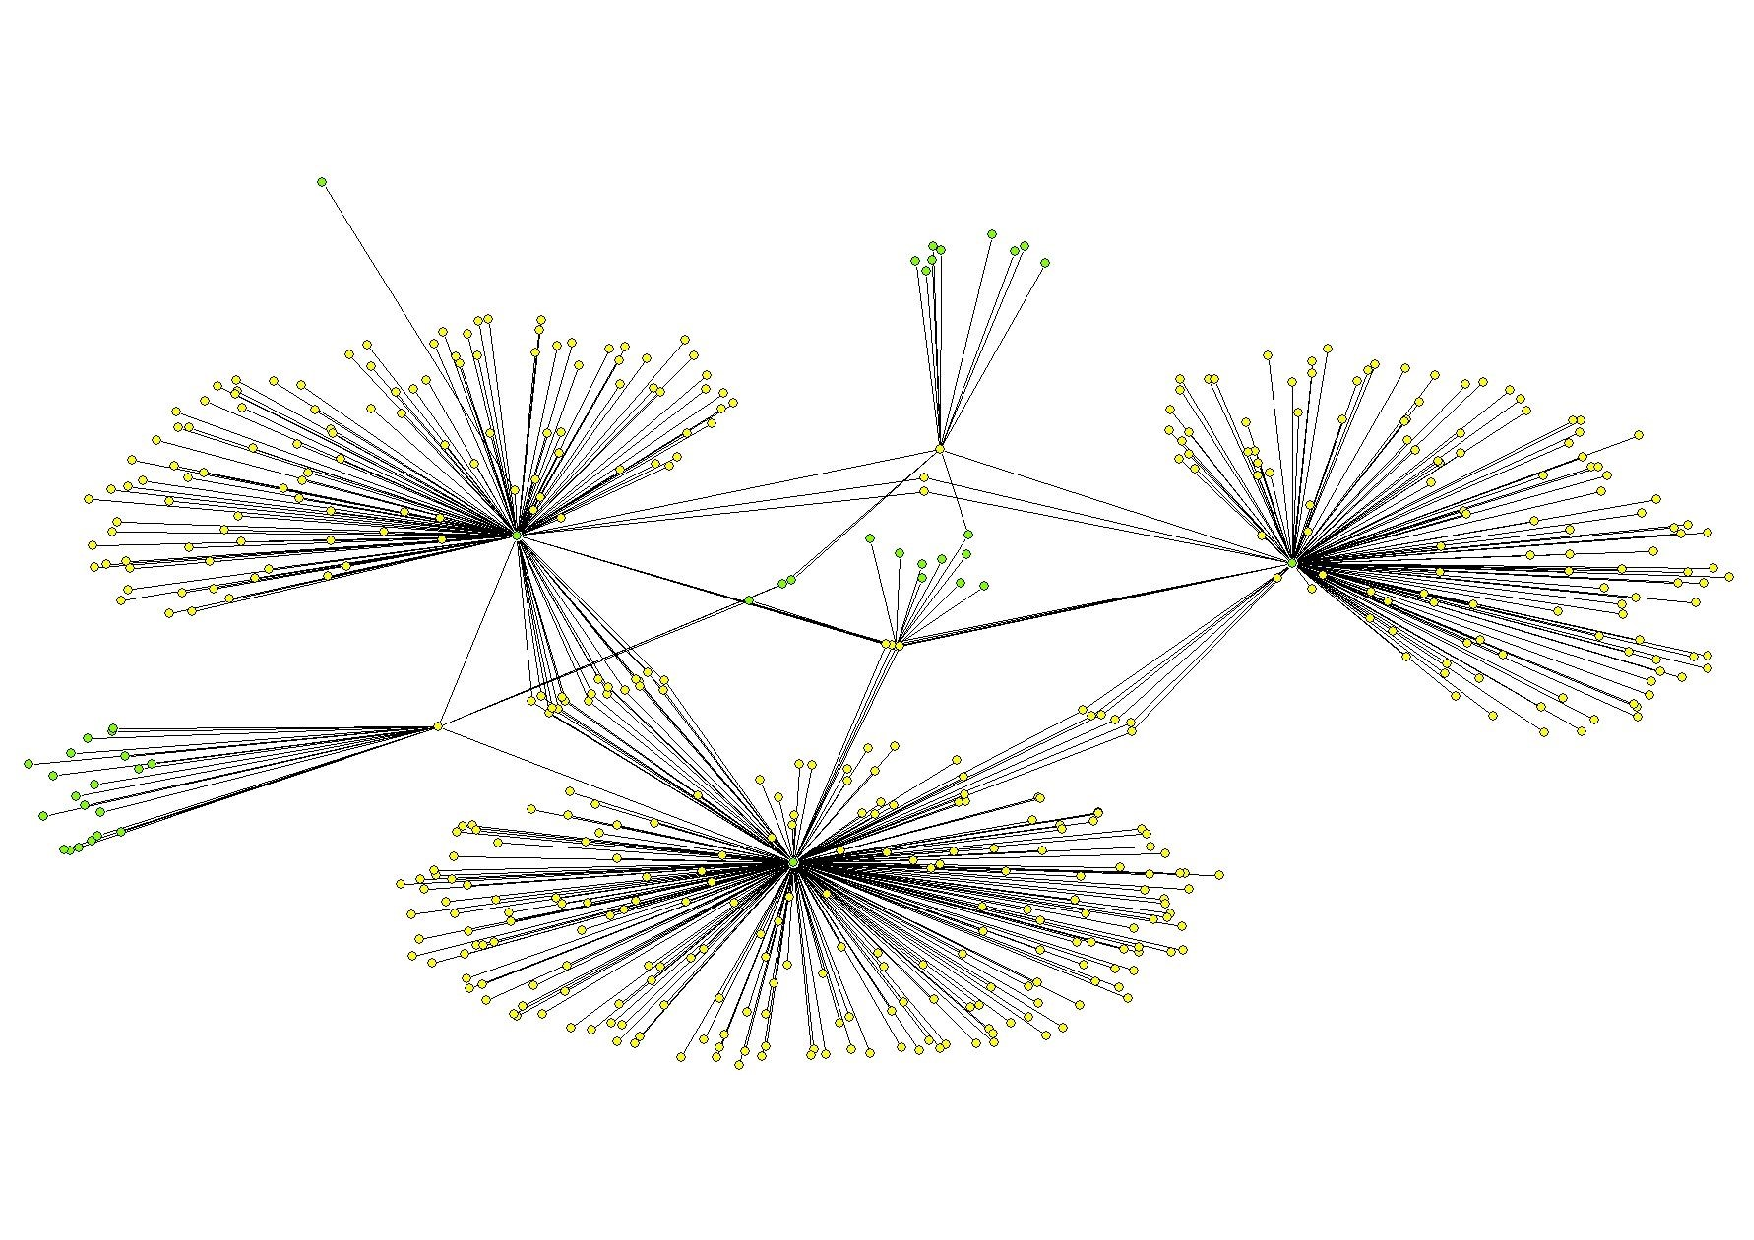
\includegraphics[scale=0.55]{rede_artistas_orquestras_PROVISORIO.pdf}
	%	\fonte{Elaboração do autor a partir de dados disponíveis online}
	%\end{figure}
	
	
	
	\postextual
	\citeoption{abnt-full-initials=yes}
	\bibliography{BIBDOUTORADO, abnt-options}
	
	
	
	
	
	
	
	%\newpage
	%\anexoname  \section*{Trabalhos Consultados}
	%\SingleSpacing
	%\footnotesize
	%\centering
	%\begin{longtable}{p{4cm}lp{4cm}p{4cm}}
	%	\hline
	%	\textbf{Autores} &\textbf{Ano} & \textbf{Journal} & \textbf{Assunto}\\
	%	\hline
	%	\hline
	%	\endfirsthead
	%	\hline
	%	\endhead
	%	\hline
	%	\endfoot
	%	\hline
	%	\hline
	%	\endlastfoot
	
	%	Roy, Tirthankar & 1998 & Contributions to Indian Sociology & Indian classical music\\
	%	Waterman, Stanley & 2010 & Contemporary Jewry & Israel culture/music\\
	%	Coaldrake, Kimi	& 2012 & Japanese Studies & Japanese popular music\\
	%	Menger, Pierre-Michel & 1991 & Cahiers de recherche sociologique & Factors affecting market structure and music evaluation\\
	%	Menger, Pierre-Michel & 1983 & Sociologie du Travail & Division of musical labor\\
	%	Buchholz, Larissa & 2013 & NA & Global rules of art\\
	%	Etzioni, Amitai & 1998 & Journal of Socio-Economics & Taste for classical music\\
	%	Roebuck, James C & 2000 & American Sociological Association & Gendered-habitus, and the sexual division of labor\\
	%	Francois, Pierre & 2004 & Sociologie du Travail & Ilness of cost / concert market / musicians labor market\\
	%	Gligorijevic, Jelena & 2014 & International Journal of Cultural Policy & Music festival / Serbia\\
	%	Hofman, Ana & 2014 & Dve domovini / Two Homelands & Identification and affiliation / trumpet orchestra music / Balkan music\\
	%	Segnini, Liliana Rolfsen Petrilli & 2011 & Estudos de Sociologia & Music work market\\
	%	Epstein, Louis K & 2013 & NA & Music patronage\\
	%	Kaleta, Andrzej & 2004 & Polish Sociological Review & Cultural Activity of Rural Inhabitants\\
	%	Zolberg, Vera & 1996 & International Sociology & Music patronage\\
	%	Mauskapf, Michael G & 2012 & NA & Music patronage / economic and cultural sustainability\\
	%	Borowiecki, Karol J; O'Hagan, John W & 2012 & Historical Social Research/Historische Sozialforschung & Historical Patterns / The case of classical composers\\
	%	Fisher, Timothy C G; Preece, Stephen B & 2003 & Poetics & Culture of comsumption\\
	%	Dowd, Timothy J; Liddle, Kathleen; Lupo, Kim; Borden, Anne. & 2002 & Poetics & Musical Canon\\
	%	Kremp, Pierre-Antoine & 2010 & Social Forces & Musical Canon\\
	%	Broughton, Andrea & 2001 & European Journal of Industrial Relations & Collective Bargaining in the Arts and Culture Sector\\
	%	Hughes, Patricia; Luksetich, William; Rooney, Patrick & 2014 & Nonprofit Management \& Leadership & Music patronage\\
	%	Glynn, Mary Ann & 2002 & Poetics & Organizational Crisis / Institutional Shifts / Musical Canon\\
	%	Wood, Roy D & 2010 & NA & Conductor leadership style, musician employment status, organizational participation to orchestra musician job satisfaction\\
	%	Bijsterveld, Karin; Schulp, Marten & 2004 & Social Studies of Science & Innovation in classical music instruments\\
	%	Luthje, Corinna & 2010 & Medien \& Kommunikationswissenschaft & Classical Music in German Commercial Radio Programming\\
	%	McCormick, Lisa & 2009 & Cultural Sociology & International Music Competition\\
	%	Lee, Steve Sungchu & 2007 & NA & Musical stratification / aesthetics\\
	%	Francois, Pierre & 2006 & Revue francaise de Sociologie & Early Music Market\\
	%	Santoro, Marco & 2013 & European Societies & Institutions / music market\\
	%	Abreu, Paula & 2009 & Revista Critica de Ciencias Sociais & Portuguese phonographic industry\\
	%	Watson, Allan & 2012 & Global Networks & Urban networks of music production / Itunes\\
	%	Nicolau, Michel & 2010 & International Sociological Association & National Identity / Brazilian music\\
	%	Janowska, Anna Anetta & 2011 & Societes & Digital Revolution / Reconrding Industry\\
	%	Abreu, Paula & 2004 & Revista Critica de Ciencias Sociais & Territorial dynamics of cultural markets / Portuguese music\\
	%	Shin, Eui Hang; Oh, Joong-Hwan & 2002 & East Asia: An International Quarterly & Relationships between two different sets of actors - songwriters \& singers / Korean popular music industry\\
	%	Salganik, Matthew J; Watts, Duncan J & 2008 & Social Psychology Quarterly & Self-fulfilling Prophecies in an Artificial Cultural Market\\
	%	Dowd, Timothy J & 2003 & Comparative Social Research & Structural Power and the Construction of Markets / R\&B\\
	%	DeNora, Tia & 2013 & European Societies & Markets and socio-cultural practices\\
	%	Menger, Pierre-Michel & 2002 & Annales & Genius / Beethoven\\
	%	Pethig, Rudiger; Cheng, Sao-Wen & 2002 & Schmollers Jahrbuch & Cultural Capital / Consumption of Cultural Services\\
	%	Salganik, Matthew J & 2007 & NA & Success and failure in cultural markets\\
	%	Kasaras, Kostas; Klimis, George Michael; Michailidou, Martha & 2012 & Contemporary Social Science: Journal of the Academy of Social Sciences & Musical tastes / experimental study\\
	%	Ginsburgh, Victor & 2003 & Journal of Economic Perspectives & Expertise in the arts influence success\\
	
	%\end{longtable}
	
\end{document}